\documentclass[twoside]{book}

% Packages required by doxygen
\usepackage{fixltx2e}
\usepackage{calc}
\usepackage{doxygen}
\usepackage[export]{adjustbox} % also loads graphicx
\usepackage{graphicx}
\usepackage[utf8]{inputenc}
\usepackage{makeidx}
\usepackage{multicol}
\usepackage{multirow}
\PassOptionsToPackage{warn}{textcomp}
\usepackage{textcomp}
\usepackage[nointegrals]{wasysym}
\usepackage[table]{xcolor}

% Font selection
\usepackage[T1]{fontenc}
\usepackage[scaled=.90]{helvet}
\usepackage{courier}
\usepackage{amssymb}
\usepackage{sectsty}
\renewcommand{\familydefault}{\sfdefault}
\allsectionsfont{%
  \fontseries{bc}\selectfont%
  \color{darkgray}%
}
\renewcommand{\DoxyLabelFont}{%
  \fontseries{bc}\selectfont%
  \color{darkgray}%
}
\newcommand{\+}{\discretionary{\mbox{\scriptsize$\hookleftarrow$}}{}{}}

% Page & text layout
\usepackage{geometry}
\geometry{%
  a4paper,%
  top=2.5cm,%
  bottom=2.5cm,%
  left=2.5cm,%
  right=2.5cm%
}
\tolerance=750
\hfuzz=15pt
\hbadness=750
\setlength{\emergencystretch}{15pt}
\setlength{\parindent}{0cm}
\setlength{\parskip}{0.2cm}
\makeatletter
\renewcommand{\paragraph}{%
  \@startsection{paragraph}{4}{0ex}{-1.0ex}{1.0ex}{%
    \normalfont\normalsize\bfseries\SS@parafont%
  }%
}
\renewcommand{\subparagraph}{%
  \@startsection{subparagraph}{5}{0ex}{-1.0ex}{1.0ex}{%
    \normalfont\normalsize\bfseries\SS@subparafont%
  }%
}
\makeatother

% Headers & footers
\usepackage{fancyhdr}
\pagestyle{fancyplain}
\fancyhead[LE]{\fancyplain{}{\bfseries\thepage}}
\fancyhead[CE]{\fancyplain{}{}}
\fancyhead[RE]{\fancyplain{}{\bfseries\leftmark}}
\fancyhead[LO]{\fancyplain{}{\bfseries\rightmark}}
\fancyhead[CO]{\fancyplain{}{}}
\fancyhead[RO]{\fancyplain{}{\bfseries\thepage}}
\fancyfoot[LE]{\fancyplain{}{}}
\fancyfoot[CE]{\fancyplain{}{}}
\fancyfoot[RE]{\fancyplain{}{\bfseries\scriptsize Generated on Sun Oct 4 2015 21\+:57\+:14 for Icon\+Magic by Doxygen }}
\fancyfoot[LO]{\fancyplain{}{\bfseries\scriptsize Generated on Sun Oct 4 2015 21\+:57\+:14 for Icon\+Magic by Doxygen }}
\fancyfoot[CO]{\fancyplain{}{}}
\fancyfoot[RO]{\fancyplain{}{}}
\renewcommand{\footrulewidth}{0.4pt}
\renewcommand{\chaptermark}[1]{%
  \markboth{#1}{}%
}
\renewcommand{\sectionmark}[1]{%
  \markright{\thesection\ #1}%
}

% Indices & bibliography
\usepackage{natbib}
\usepackage[titles]{tocloft}
\setcounter{tocdepth}{3}
\setcounter{secnumdepth}{5}
\makeindex

% Hyperlinks (required, but should be loaded last)
\usepackage{ifpdf}
\ifpdf
  \usepackage[pdftex,pagebackref=true]{hyperref}
\else
  \usepackage[ps2pdf,pagebackref=true]{hyperref}
\fi
\hypersetup{%
  colorlinks=true,%
  linkcolor=blue,%
  citecolor=blue,%
  unicode%
}

% Custom commands
\newcommand{\clearemptydoublepage}{%
  \newpage{\pagestyle{empty}\cleardoublepage}%
}


%===== C O N T E N T S =====

\begin{document}

% Titlepage & ToC
\hypersetup{pageanchor=false,
             bookmarks=true,
             bookmarksnumbered=true,
             pdfencoding=unicode
            }
\pagenumbering{roman}
\begin{titlepage}
\vspace*{7cm}
\begin{center}%
{\Large Icon\+Magic \\[1ex]\large 0.\+1 }\\
\vspace*{1cm}
{\large Generated by Doxygen 1.8.10}\\
\vspace*{0.5cm}
{\small Sun Oct 4 2015 21:57:14}\\
\end{center}
\end{titlepage}
\clearemptydoublepage
\tableofcontents
\clearemptydoublepage
\pagenumbering{arabic}
\hypersetup{pageanchor=true}

%--- Begin generated contents ---
\chapter{Main Page}
\label{index}\hypertarget{index}{}\section*{Icon\+Magic}

You can find this project on its Git\+Hub \href{https://github.com/ThetaSinner/IconMagic}{\tt page}

\subsubsection*{The plan}

The aim of the Icon\+Magic is to make it super simple to change file icons in Windows.

Features
\begin{DoxyItemize}
\item Able to perform a complete scan of the registry to find existing references to icons.
\item The user can easily change the icon a registry key is pointing to.
\item Keeps a complete history of every change you make. The history file can be used to
\begin{DoxyItemize}
\item Roll back a change.
\item Revert all changes to a file type.
\end{DoxyItemize}
\end{DoxyItemize}

\subsubsection*{Future ideas}


\begin{DoxyItemize}
\item The user should be able to add a new new file type to the registry and set its icon. 
\end{DoxyItemize}
\chapter{Icon\+Magic license.}
\label{license}
\hypertarget{license}{}
\hypertarget{license_license_section}{}\section{Icon\+Magic}\label{license_license_section}
\begin{DoxyAuthor}{Author}
Theta\+Sinner (Gregory Jensen) 
\end{DoxyAuthor}
\begin{DoxyCopyright}{Copyright}
The license can be found \href{https://github.com/ThetaSinner/IconMagic/blob/master/LICENSE}{\tt here}. 
\end{DoxyCopyright}

\chapter{Todo List}
\label{todo}
\hypertarget{todo}{}

\begin{DoxyRefList}
\item[\label{todo__todo000001}%
\hypertarget{todo__todo000001}{}%
Member \hyperlink{class_test_framework_a4f37e58d8b67f9da66372cf43f4281ae}{Test\+Framework\+:\+:add\+Test} (std\+::function$<$ bool(void)$>$ test\+Function)]\+: document this function  
\item[\label{todo__todo000002}%
\hypertarget{todo__todo000002}{}%
Member \hyperlink{class_test_framework_ace2588c0b0043546abc584b1d1b08e96}{Test\+Framework\+:\+:execute} ()]\+: document this function  
\item[\label{todo__todo000003}%
\hypertarget{todo__todo000003}{}%
Member \hyperlink{class_test_framework_ae12aac94ee9a745eb3ce46f5d003dcf2}{Test\+Framework\+:\+:get\+Tests\+Status} ()]\+: document this function  
\item[\label{todo__todo000004}%
\hypertarget{todo__todo000004}{}%
Member \hyperlink{class_test_framework_ad35b7b750378155531cf65e8163b67dd}{Test\+Framework\+:\+:get\+Total\+Tests\+Run} ()]\+: document this function  
\item[\label{todo__todo000005}%
\hypertarget{todo__todo000005}{}%
Member \hyperlink{class_test_framework_a34508c693cf7a3be01a3975065fa2457}{Test\+Framework\+:\+:get\+Total\+Tests\+Run\+Successfully} ()]\+: document this function  
\item[\label{todo__todo000006}%
\hypertarget{todo__todo000006}{}%
Member \hyperlink{class_test_framework_a80e30a085718a9e3db4e6f4e79cc9d48}{Test\+Framework\+:\+:Test\+Framework} ()]\+: document this function  
\item[\label{todo__todo000007}%
\hypertarget{todo__todo000007}{}%
Member \hyperlink{class_test_framework_aad3d6888fe40a083e767061a1ebf0c1d}{Test\+Framework\+:\+:$\sim$\+Test\+Framework} ()]\+: document this function 
\end{DoxyRefList}
\chapter{Hierarchical Index}
\section{Class Hierarchy}
This inheritance list is sorted roughly, but not completely, alphabetically\+:\begin{DoxyCompactList}
\item \contentsline{section}{Direct\+Registry\+Access}{\pageref{class_direct_registry_access}}{}
\item \contentsline{section}{Example\+Class}{\pageref{class_example_class}}{}
\item exception\begin{DoxyCompactList}
\item \contentsline{section}{Registry\+Access\+Exception}{\pageref{class_registry_access_exception}}{}
\item \contentsline{section}{Registry\+Scan\+Exception}{\pageref{class_registry_scan_exception}}{}
\end{DoxyCompactList}
\item \contentsline{section}{Extension\+History}{\pageref{class_extension_history}}{}
\item \contentsline{section}{Image\+Entry}{\pageref{class_image_entry}}{}
\item \contentsline{section}{Key\+Path}{\pageref{class_key_path}}{}
\item \contentsline{section}{Key\+Service}{\pageref{class_key_service}}{}
\item \contentsline{section}{Manager}{\pageref{class_manager}}{}
\item \contentsline{section}{Menu}{\pageref{class_menu}}{}
\begin{DoxyCompactList}
\item \contentsline{section}{Menu\+Branch}{\pageref{class_menu_branch}}{}
\item \contentsline{section}{Menu\+Leaf}{\pageref{class_menu_leaf}}{}
\begin{DoxyCompactList}
\item \contentsline{section}{Menu\+Exit}{\pageref{class_menu_exit}}{}
\end{DoxyCompactList}
\end{DoxyCompactList}
\item \contentsline{section}{Menu\+Factory}{\pageref{class_menu_factory}}{}
\item \contentsline{section}{Menu\+Manager}{\pageref{class_menu_manager}}{}
\item \contentsline{section}{Registry\+History}{\pageref{class_registry_history}}{}
\item \contentsline{section}{Registry\+Scanner}{\pageref{class_registry_scanner}}{}
\item \contentsline{section}{Scan\+Tool}{\pageref{class_scan_tool}}{}
\item \contentsline{section}{Simple\+Registry\+Access}{\pageref{class_simple_registry_access}}{}
\item \contentsline{section}{Test\+Framework}{\pageref{class_test_framework}}{}
\end{DoxyCompactList}

\chapter{Class Index}
\section{Class List}
Here are the classes, structs, unions and interfaces with brief descriptions\+:\begin{DoxyCompactList}
\item\contentsline{section}{\hyperlink{class_direct_registry_access}{Direct\+Registry\+Access} \\*Wrapper for Windows A\+P\+I registry access }{\pageref{class_direct_registry_access}}{}
\item\contentsline{section}{\hyperlink{class_example_class}{Example\+Class} \\*An example class }{\pageref{class_example_class}}{}
\item\contentsline{section}{\hyperlink{class_extension_history}{Extension\+History} }{\pageref{class_extension_history}}{}
\item\contentsline{section}{\hyperlink{class_image_entry}{Image\+Entry} \\*Class for manipulating icon references as they appear in the registry }{\pageref{class_image_entry}}{}
\item\contentsline{section}{\hyperlink{class_key_path}{Key\+Path} \\*Object representation of a registry path }{\pageref{class_key_path}}{}
\item\contentsline{section}{\hyperlink{class_key_service}{Key\+Service} \\*Provides a key lookup service }{\pageref{class_key_service}}{}
\item\contentsline{section}{\hyperlink{class_manager}{Manager} }{\pageref{class_manager}}{}
\item\contentsline{section}{\hyperlink{class_menu}{Menu} }{\pageref{class_menu}}{}
\item\contentsline{section}{\hyperlink{class_menu_branch}{Menu\+Branch} }{\pageref{class_menu_branch}}{}
\item\contentsline{section}{\hyperlink{class_menu_exit}{Menu\+Exit} }{\pageref{class_menu_exit}}{}
\item\contentsline{section}{\hyperlink{class_menu_factory}{Menu\+Factory} }{\pageref{class_menu_factory}}{}
\item\contentsline{section}{\hyperlink{class_menu_leaf}{Menu\+Leaf} }{\pageref{class_menu_leaf}}{}
\item\contentsline{section}{\hyperlink{class_menu_manager}{Menu\+Manager} }{\pageref{class_menu_manager}}{}
\item\contentsline{section}{\hyperlink{class_registry_access_exception}{Registry\+Access\+Exception} }{\pageref{class_registry_access_exception}}{}
\item\contentsline{section}{\hyperlink{class_registry_history}{Registry\+History} }{\pageref{class_registry_history}}{}
\item\contentsline{section}{\hyperlink{class_registry_scan_exception}{Registry\+Scan\+Exception} }{\pageref{class_registry_scan_exception}}{}
\item\contentsline{section}{\hyperlink{class_registry_scanner}{Registry\+Scanner} }{\pageref{class_registry_scanner}}{}
\item\contentsline{section}{\hyperlink{class_scan_tool}{Scan\+Tool} }{\pageref{class_scan_tool}}{}
\item\contentsline{section}{\hyperlink{class_simple_registry_access}{Simple\+Registry\+Access} \\*Extends the functionality of \hyperlink{class_direct_registry_access}{Direct\+Registry\+Access} }{\pageref{class_simple_registry_access}}{}
\item\contentsline{section}{\hyperlink{class_test_framework}{Test\+Framework} }{\pageref{class_test_framework}}{}
\end{DoxyCompactList}

\chapter{File Index}
\section{File List}
Here is a list of all documented files with brief descriptions\+:\begin{DoxyCompactList}
\item\contentsline{section}{D\+:/\+Users/\+Gregory/\+One\+Drive/\+Git\+Hub/\+Icon\+Magic/\+Source/\hyperlink{main_8cpp}{main.\+cpp} \\*Created by Theta\+Sinner (Gregory Jensen). Released as open source }{\pageref{main_8cpp}}{}
\item\contentsline{section}{D\+:/\+Users/\+Gregory/\+One\+Drive/\+Git\+Hub/\+Icon\+Magic/\+Source/doc/{\bfseries index.\+hpp} }{\pageref{index_8hpp}}{}
\item\contentsline{section}{D\+:/\+Users/\+Gregory/\+One\+Drive/\+Git\+Hub/\+Icon\+Magic/\+Source/doc/{\bfseries license.\+hpp} }{\pageref{license_8hpp}}{}
\item\contentsline{section}{D\+:/\+Users/\+Gregory/\+One\+Drive/\+Git\+Hub/\+Icon\+Magic/\+Source/doxygen/\hyperlink{example_8hpp}{example.\+hpp} \\*Examples of the doxygen markup I plan to use accross the project }{\pageref{example_8hpp}}{}
\item\contentsline{section}{D\+:/\+Users/\+Gregory/\+One\+Drive/\+Git\+Hub/\+Icon\+Magic/\+Source/main/\hyperlink{_icon_magic_8cpp}{Icon\+Magic.\+cpp} \\*Created by Theta\+Sinner (Gregory Jensen). Released as open source }{\pageref{_icon_magic_8cpp}}{}
\item\contentsline{section}{D\+:/\+Users/\+Gregory/\+One\+Drive/\+Git\+Hub/\+Icon\+Magic/\+Source/main/\hyperlink{_icon_magic_8hpp}{Icon\+Magic.\+hpp} \\*Created by Theta\+Sinner (Gregory Jensen). Released as open source }{\pageref{_icon_magic_8hpp}}{}
\item\contentsline{section}{D\+:/\+Users/\+Gregory/\+One\+Drive/\+Git\+Hub/\+Icon\+Magic/\+Source/main/\hyperlink{_manager_8cpp}{Manager.\+cpp} \\*Created by Theta\+Sinner (Gregory Jensen). Released as open source }{\pageref{_manager_8cpp}}{}
\item\contentsline{section}{D\+:/\+Users/\+Gregory/\+One\+Drive/\+Git\+Hub/\+Icon\+Magic/\+Source/main/\hyperlink{_manager_8hpp}{Manager.\+hpp} \\*Created by Theta\+Sinner (Gregory Jensen). Released as open source }{\pageref{_manager_8hpp}}{}
\item\contentsline{section}{D\+:/\+Users/\+Gregory/\+One\+Drive/\+Git\+Hub/\+Icon\+Magic/\+Source/main/\hyperlink{_system_validation_8cpp}{System\+Validation.\+cpp} \\*Created by Theta\+Sinner (Gregory Jensen). Released as open source }{\pageref{_system_validation_8cpp}}{}
\item\contentsline{section}{D\+:/\+Users/\+Gregory/\+One\+Drive/\+Git\+Hub/\+Icon\+Magic/\+Source/main/\hyperlink{_system_validation_8hpp}{System\+Validation.\+hpp} \\*Created by Theta\+Sinner (Gregory Jensen). Released as open source }{\pageref{_system_validation_8hpp}}{}
\item\contentsline{section}{D\+:/\+Users/\+Gregory/\+One\+Drive/\+Git\+Hub/\+Icon\+Magic/\+Source/main/\hyperlink{_text_u_i_8cpp}{Text\+U\+I.\+cpp} \\*Created by Theta\+Sinner (Gregory Jensen). Released as open source }{\pageref{_text_u_i_8cpp}}{}
\item\contentsline{section}{D\+:/\+Users/\+Gregory/\+One\+Drive/\+Git\+Hub/\+Icon\+Magic/\+Source/main/\hyperlink{_text_u_i_8hpp}{Text\+U\+I.\+hpp} \\*Created by Theta\+Sinner (Gregory Jensen). Released as open source }{\pageref{_text_u_i_8hpp}}{}
\item\contentsline{section}{D\+:/\+Users/\+Gregory/\+One\+Drive/\+Git\+Hub/\+Icon\+Magic/\+Source/main/{\bfseries Util.\+hpp} }{\pageref{_util_8hpp}}{}
\item\contentsline{section}{D\+:/\+Users/\+Gregory/\+One\+Drive/\+Git\+Hub/\+Icon\+Magic/\+Source/main/\hyperlink{_windows_toolbox_8cpp}{Windows\+Toolbox.\+cpp} \\*Created by Theta\+Sinner (Gregory Jensen). Released as open source }{\pageref{_windows_toolbox_8cpp}}{}
\item\contentsline{section}{D\+:/\+Users/\+Gregory/\+One\+Drive/\+Git\+Hub/\+Icon\+Magic/\+Source/main/\hyperlink{_windows_toolbox_8hpp}{Windows\+Toolbox.\+hpp} \\*Created by Theta\+Sinner (Gregory Jensen). Released as open source }{\pageref{_windows_toolbox_8hpp}}{}
\item\contentsline{section}{D\+:/\+Users/\+Gregory/\+One\+Drive/\+Git\+Hub/\+Icon\+Magic/\+Source/main/\+Menu/{\bfseries Menu.\+hpp} }{\pageref{_menu_8hpp}}{}
\item\contentsline{section}{D\+:/\+Users/\+Gregory/\+One\+Drive/\+Git\+Hub/\+Icon\+Magic/\+Source/main/\+Menu/{\bfseries Menu\+Manager.\+hpp} }{\pageref{_menu_manager_8hpp}}{}
\item\contentsline{section}{D\+:/\+Users/\+Gregory/\+One\+Drive/\+Git\+Hub/\+Icon\+Magic/\+Source/main/\+Menu/\+Menu\+Definitions/{\bfseries Menu\+Factory.\+hpp} }{\pageref{_menu_factory_8hpp}}{}
\item\contentsline{section}{D\+:/\+Users/\+Gregory/\+One\+Drive/\+Git\+Hub/\+Icon\+Magic/\+Source/main/\+Registry/\+Common/\hyperlink{_key_path_8cpp}{Key\+Path.\+cpp} \\*The \hyperlink{class_key_path}{Key\+Path} class implementation }{\pageref{_key_path_8cpp}}{}
\item\contentsline{section}{D\+:/\+Users/\+Gregory/\+One\+Drive/\+Git\+Hub/\+Icon\+Magic/\+Source/main/\+Registry/\+Common/\hyperlink{_key_path_8hpp}{Key\+Path.\+hpp} \\*The \hyperlink{class_key_path}{Key\+Path} class definition }{\pageref{_key_path_8hpp}}{}
\item\contentsline{section}{D\+:/\+Users/\+Gregory/\+One\+Drive/\+Git\+Hub/\+Icon\+Magic/\+Source/main/\+Registry/\+Common/\hyperlink{_key_service_8cpp}{Key\+Service.\+cpp} \\*The \hyperlink{class_key_service}{Key\+Service} class implementation }{\pageref{_key_service_8cpp}}{}
\item\contentsline{section}{D\+:/\+Users/\+Gregory/\+One\+Drive/\+Git\+Hub/\+Icon\+Magic/\+Source/main/\+Registry/\+Common/\hyperlink{_key_service_8hpp}{Key\+Service.\+hpp} \\*The \hyperlink{class_key_service}{Key\+Service} class definition }{\pageref{_key_service_8hpp}}{}
\item\contentsline{section}{D\+:/\+Users/\+Gregory/\+One\+Drive/\+Git\+Hub/\+Icon\+Magic/\+Source/main/\+Registry/\+Data\+Access/{\bfseries Direct\+Registry\+Access.\+hpp} }{\pageref{_direct_registry_access_8hpp}}{}
\item\contentsline{section}{D\+:/\+Users/\+Gregory/\+One\+Drive/\+Git\+Hub/\+Icon\+Magic/\+Source/main/\+Registry/\+Data\+Access/{\bfseries Registry\+Access\+Exception.\+hpp} }{\pageref{_registry_access_exception_8hpp}}{}
\item\contentsline{section}{D\+:/\+Users/\+Gregory/\+One\+Drive/\+Git\+Hub/\+Icon\+Magic/\+Source/main/\+Registry/\+Data\+Access/{\bfseries Simple\+Registry\+Access.\+hpp} }{\pageref{_simple_registry_access_8hpp}}{}
\item\contentsline{section}{D\+:/\+Users/\+Gregory/\+One\+Drive/\+Git\+Hub/\+Icon\+Magic/\+Source/main/\+Registry/\+History/{\bfseries Extension\+History.\+hpp} }{\pageref{_extension_history_8hpp}}{}
\item\contentsline{section}{D\+:/\+Users/\+Gregory/\+One\+Drive/\+Git\+Hub/\+Icon\+Magic/\+Source/main/\+Registry/\+History/{\bfseries Image\+Entry.\+hpp} }{\pageref{_image_entry_8hpp}}{}
\item\contentsline{section}{D\+:/\+Users/\+Gregory/\+One\+Drive/\+Git\+Hub/\+Icon\+Magic/\+Source/main/\+Registry/\+History/\hyperlink{_registry_history_8cpp}{Registry\+History.\+cpp} \\*Record changes to \textquotesingle{}Default\+Icon\textquotesingle{} keys in the registry using a custom file format }{\pageref{_registry_history_8cpp}}{}
\item\contentsline{section}{D\+:/\+Users/\+Gregory/\+One\+Drive/\+Git\+Hub/\+Icon\+Magic/\+Source/main/\+Registry/\+History/{\bfseries Registry\+History.\+hpp} }{\pageref{_registry_history_8hpp}}{}
\item\contentsline{section}{D\+:/\+Users/\+Gregory/\+One\+Drive/\+Git\+Hub/\+Icon\+Magic/\+Source/main/\+Registry/\+Scanner/{\bfseries Registry\+Scanner.\+hpp} }{\pageref{_registry_scanner_8hpp}}{}
\item\contentsline{section}{D\+:/\+Users/\+Gregory/\+One\+Drive/\+Git\+Hub/\+Icon\+Magic/\+Source/main/\+Registry/\+Scanner/{\bfseries Scan\+Tool.\+hpp} }{\pageref{_scan_tool_8hpp}}{}
\item\contentsline{section}{D\+:/\+Users/\+Gregory/\+One\+Drive/\+Git\+Hub/\+Icon\+Magic/\+Source/test/\hyperlink{framework_8cpp}{framework.\+cpp} \\*Created by Theta\+Sinner (Gregory Jensen). Released as open source }{\pageref{framework_8cpp}}{}
\item\contentsline{section}{D\+:/\+Users/\+Gregory/\+One\+Drive/\+Git\+Hub/\+Icon\+Magic/\+Source/test/{\bfseries framework.\+hpp} }{\pageref{framework_8hpp}}{}
\item\contentsline{section}{D\+:/\+Users/\+Gregory/\+One\+Drive/\+Git\+Hub/\+Icon\+Magic/\+Source/test/\hyperlink{_testing_8cpp}{Testing.\+cpp} \\*Created by Theta\+Sinner (Gregory Jensen). Released as open source }{\pageref{_testing_8cpp}}{}
\item\contentsline{section}{D\+:/\+Users/\+Gregory/\+One\+Drive/\+Git\+Hub/\+Icon\+Magic/\+Source/test/\hyperlink{_testing_8hpp}{Testing.\+hpp} \\*Created by Theta\+Sinner (Gregory Jensen). Released as open source }{\pageref{_testing_8hpp}}{}
\item\contentsline{section}{D\+:/\+Users/\+Gregory/\+One\+Drive/\+Git\+Hub/\+Icon\+Magic/\+Source/test/\+Registry\+History/\hyperlink{_registry_history_test_8cpp}{Registry\+History\+Test.\+cpp} \\*Created by Theta\+Sinner (Gregory Jensen). Released as open source }{\pageref{_registry_history_test_8cpp}}{}
\item\contentsline{section}{D\+:/\+Users/\+Gregory/\+One\+Drive/\+Git\+Hub/\+Icon\+Magic/\+Source/test/\+Registry\+History/{\bfseries Registry\+History\+Test.\+hpp} }{\pageref{_registry_history_test_8hpp}}{}
\end{DoxyCompactList}

\chapter{Class Documentation}
\hypertarget{class_direct_registry_access}{}\section{Direct\+Registry\+Access Class Reference}
\label{class_direct_registry_access}\index{Direct\+Registry\+Access@{Direct\+Registry\+Access}}


Wrapper for Windows A\+P\+I registry access.  




{\ttfamily \#include $<$Direct\+Registry\+Access.\+hpp$>$}

Inheritance diagram for Direct\+Registry\+Access\+:\begin{figure}[H]
\begin{center}
\leavevmode
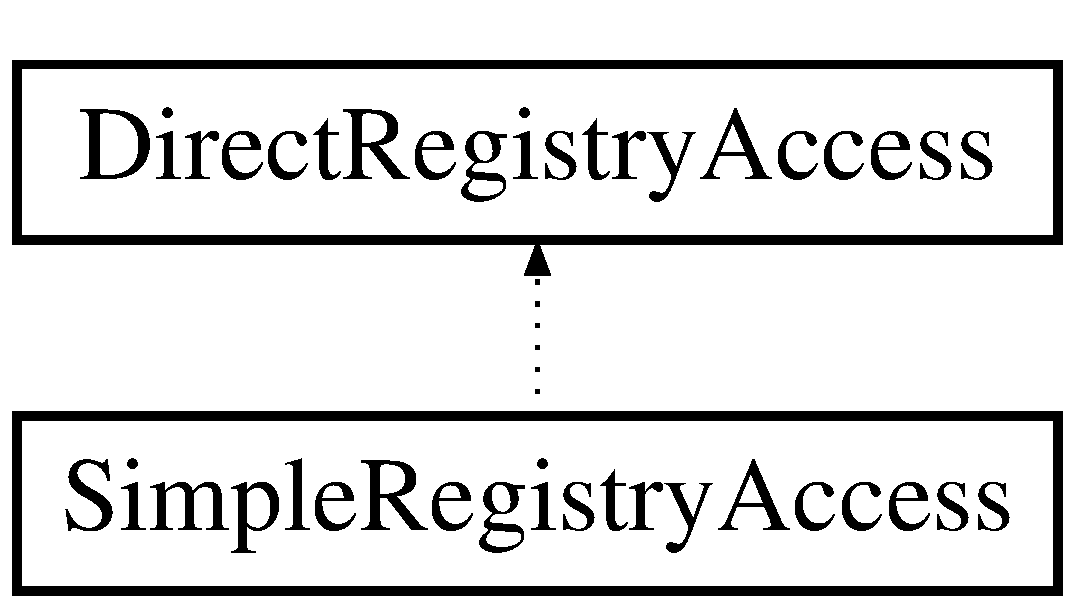
\includegraphics[height=2.000000cm]{class_direct_registry_access}
\end{center}
\end{figure}
\subsection*{Static Public Member Functions}
\begin{DoxyCompactItemize}
\item 
static bool \hyperlink{class_direct_registry_access_ae051be8724359399dacc86a38149762c}{open\+Key\+For\+Enumeration} (H\+K\+E\+Y root\+\_\+key, std\+::string path, H\+K\+E\+Y \&h\+\_\+key)
\begin{DoxyCompactList}\small\item\em Open a key for reading. \end{DoxyCompactList}\item 
static bool \hyperlink{class_direct_registry_access_affd3141655ca0d587461282fcab5cc25}{open\+Key\+For\+Enumeration} (H\+K\+E\+Y root\+\_\+key, H\+K\+E\+Y \&h\+\_\+key)
\begin{DoxyCompactList}\small\item\em Shortcut. \end{DoxyCompactList}\item 
static bool \hyperlink{class_direct_registry_access_a3bef2793ed202b4ba02ad9e099785485}{open\+Key\+For\+Setting\+Value} (H\+K\+E\+Y root\+\_\+key, std\+::string path, H\+K\+E\+Y \&h\+\_\+key)
\begin{DoxyCompactList}\small\item\em Open a registry key for writing. \end{DoxyCompactList}\item 
static bool \hyperlink{class_direct_registry_access_aa123bf857d78ceb45ef406535869c6b1}{get\+Sub\+Key\+Name\+At} (const H\+K\+E\+Y \&root\+\_\+key, int n, std\+::string \&key\+\_\+name)
\begin{DoxyCompactList}\small\item\em Iterate over subkeys. \end{DoxyCompactList}\item 
static bool \hyperlink{class_direct_registry_access_a0c4addcf0e776cdecead314ef7427f73}{get\+Value\+From\+Key} (H\+K\+E\+Y \&h\+\_\+key, std\+::string search\+\_\+value\+\_\+name, std\+::string $\ast$value)
\begin{DoxyCompactList}\small\item\em Get the value with the specified name from a key. \end{DoxyCompactList}\item 
static bool \hyperlink{class_direct_registry_access_a47b88eff5dfae4e37ca98b26d62dd12a}{get\+Value\+From\+Key} (H\+K\+E\+Y \&h\+\_\+key, std\+::string $\ast$value)
\begin{DoxyCompactList}\small\item\em Shortcut. \end{DoxyCompactList}\item 
static bool \hyperlink{class_direct_registry_access_a9a80842fdb2b503215fe757632d0448b}{set\+Value\+For\+Key} (H\+K\+E\+Y \&h\+\_\+key, std\+::string value\+\_\+name, std\+::string value)
\begin{DoxyCompactList}\small\item\em Set the value with the specified name on the input key. \end{DoxyCompactList}\item 
static bool \hyperlink{class_direct_registry_access_a7d09201af3a73bc290d6334fdd09ea6b}{set\+Value\+For\+Key} (H\+K\+E\+Y \&h\+\_\+key, std\+::string value)
\begin{DoxyCompactList}\small\item\em Shortcut. \end{DoxyCompactList}\item 
static void \hyperlink{class_direct_registry_access_a05d4a5bbed79beba121eddf512fda0a0}{close\+Key} (H\+K\+E\+Y \&h\+\_\+key)
\begin{DoxyCompactList}\small\item\em Close the key handle. \end{DoxyCompactList}\end{DoxyCompactItemize}


\subsection{Detailed Description}
Wrapper for Windows A\+P\+I registry access. 

All the Windows A\+P\+I functions which are related to registry access are wrapped here. There isn\textquotesingle{}t much need to expose the Windows A\+P\+I calls, most of the parameters to real calls can take their default values.

\begin{DoxySeeAlso}{See also}
\hyperlink{class_simple_registry_access}{Simple\+Registry\+Access} 
\end{DoxySeeAlso}


\subsection{Member Function Documentation}
\hypertarget{class_direct_registry_access_a05d4a5bbed79beba121eddf512fda0a0}{}\index{Direct\+Registry\+Access@{Direct\+Registry\+Access}!close\+Key@{close\+Key}}
\index{close\+Key@{close\+Key}!Direct\+Registry\+Access@{Direct\+Registry\+Access}}
\subsubsection[{close\+Key(\+H\+K\+E\+Y \&h\+\_\+key)}]{\setlength{\rightskip}{0pt plus 5cm}void Direct\+Registry\+Access\+::close\+Key (
\begin{DoxyParamCaption}
\item[{H\+K\+E\+Y \&}]{h\+\_\+key}
\end{DoxyParamCaption}
)\hspace{0.3cm}{\ttfamily [static]}}\label{class_direct_registry_access_a05d4a5bbed79beba121eddf512fda0a0}


Close the key handle. 

This should always the used to release open key handles, regardless of the flag used to open them.

The Windows A\+P\+I doesn\textquotesingle{}t reliably report the success or otherwise of this method so this method returns void.


\begin{DoxyParams}{Parameters}
{\em h\+\_\+key} & Handle to the key to be closed. \\
\hline
\end{DoxyParams}
\hypertarget{class_direct_registry_access_aa123bf857d78ceb45ef406535869c6b1}{}\index{Direct\+Registry\+Access@{Direct\+Registry\+Access}!get\+Sub\+Key\+Name\+At@{get\+Sub\+Key\+Name\+At}}
\index{get\+Sub\+Key\+Name\+At@{get\+Sub\+Key\+Name\+At}!Direct\+Registry\+Access@{Direct\+Registry\+Access}}
\subsubsection[{get\+Sub\+Key\+Name\+At(const H\+K\+E\+Y \&root\+\_\+key, int n, std\+::string \&key\+\_\+name)}]{\setlength{\rightskip}{0pt plus 5cm}bool Direct\+Registry\+Access\+::get\+Sub\+Key\+Name\+At (
\begin{DoxyParamCaption}
\item[{const H\+K\+E\+Y \&}]{root\+\_\+key, }
\item[{int}]{n, }
\item[{std\+::string \&}]{key\+\_\+name}
\end{DoxyParamCaption}
)\hspace{0.3cm}{\ttfamily [static]}}\label{class_direct_registry_access_aa123bf857d78ceb45ef406535869c6b1}


Iterate over subkeys. 

Given a key handle opened with the enumerate flag, we can fetch the name of each child key name.

If you use an index greater than the number of children a key has then the Windows A\+P\+I returns the the last key name it finds. My method will give back en empty string in this case. This is not a failure case, the method will continue to return true.


\begin{DoxyParams}{Parameters}
{\em root\+\_\+key} & A handle to a key opened with the enumerate flag. \\
\hline
{\em n} & The index of the child key to access. \\
\hline
{\em key\+\_\+name} & The name of the child key at index n will be set on this value.\\
\hline
\end{DoxyParams}
\begin{DoxyReturn}{Returns}
Depending on the success or failure of the Windows A\+P\+I call.
\end{DoxyReturn}
\begin{DoxyRefDesc}{Todo}
\item[\hyperlink{todo__todo000002}{Todo}]You can determine the buffer size required at runtime, see Reg\+Query\+Info\+Key. \end{DoxyRefDesc}
\hypertarget{class_direct_registry_access_a0c4addcf0e776cdecead314ef7427f73}{}\index{Direct\+Registry\+Access@{Direct\+Registry\+Access}!get\+Value\+From\+Key@{get\+Value\+From\+Key}}
\index{get\+Value\+From\+Key@{get\+Value\+From\+Key}!Direct\+Registry\+Access@{Direct\+Registry\+Access}}
\subsubsection[{get\+Value\+From\+Key(\+H\+K\+E\+Y \&h\+\_\+key, std\+::string search\+\_\+value\+\_\+name, std\+::string $\ast$value)}]{\setlength{\rightskip}{0pt plus 5cm}bool Direct\+Registry\+Access\+::get\+Value\+From\+Key (
\begin{DoxyParamCaption}
\item[{H\+K\+E\+Y \&}]{h\+\_\+key, }
\item[{std\+::string}]{search\+\_\+value\+\_\+name, }
\item[{std\+::string $\ast$}]{value}
\end{DoxyParamCaption}
)\hspace{0.3cm}{\ttfamily [static]}}\label{class_direct_registry_access_a0c4addcf0e776cdecead314ef7427f73}


Get the value with the specified name from a key. 

Fetch the value with the specified name from the the key handle which must be opened with a read flag.


\begin{DoxyParams}{Parameters}
{\em h\+\_\+key} & Handle to an open key. \\
\hline
{\em search\+\_\+value\+\_\+name} & The name of the value to retrieve. \\
\hline
{\em value} & The retrieved value will be set on this parameter.\\
\hline
\end{DoxyParams}
\begin{DoxyReturn}{Returns}
Depending on the success or failure of the Windows A\+P\+I call.
\end{DoxyReturn}
\begin{DoxyRefDesc}{Todo}
\item[\hyperlink{todo__todo000003}{Todo}]This method only supports string output, you can determine the type by querying the registry.\end{DoxyRefDesc}


\begin{DoxyRefDesc}{Todo}
\item[\hyperlink{todo__todo000004}{Todo}]The output parameter should be pass by reference rather than a pointer.\end{DoxyRefDesc}


\begin{DoxyRefDesc}{Todo}
\item[\hyperlink{todo__todo000005}{Todo}]You can determine the buffer size required at runtime, see Reg\+Query\+Info\+Key. \end{DoxyRefDesc}
\hypertarget{class_direct_registry_access_a47b88eff5dfae4e37ca98b26d62dd12a}{}\index{Direct\+Registry\+Access@{Direct\+Registry\+Access}!get\+Value\+From\+Key@{get\+Value\+From\+Key}}
\index{get\+Value\+From\+Key@{get\+Value\+From\+Key}!Direct\+Registry\+Access@{Direct\+Registry\+Access}}
\subsubsection[{get\+Value\+From\+Key(\+H\+K\+E\+Y \&h\+\_\+key, std\+::string $\ast$value)}]{\setlength{\rightskip}{0pt plus 5cm}bool Direct\+Registry\+Access\+::get\+Value\+From\+Key (
\begin{DoxyParamCaption}
\item[{H\+K\+E\+Y \&}]{h\+\_\+key, }
\item[{std\+::string $\ast$}]{value}
\end{DoxyParamCaption}
)\hspace{0.3cm}{\ttfamily [static]}}\label{class_direct_registry_access_a47b88eff5dfae4e37ca98b26d62dd12a}


Shortcut. 

This shortcut calls \hyperlink{class_direct_registry_access_a0c4addcf0e776cdecead314ef7427f73}{Direct\+Registry\+Access\+::get\+Value\+From\+Key(\+H\+K\+E\+Y\&, std\+::string, std\+::string$\ast$)} with an empty string as the second parameter. This tells the Windows A\+P\+I to fetch the \textquotesingle{}default\textquotesingle{} value from the input key.

\begin{DoxySeeAlso}{See also}
\hyperlink{class_direct_registry_access_a0c4addcf0e776cdecead314ef7427f73}{Direct\+Registry\+Access\+::get\+Value\+From\+Key(\+H\+K\+E\+Y\&, std\+::string, std\+::string$\ast$)} 
\end{DoxySeeAlso}
\hypertarget{class_direct_registry_access_ae051be8724359399dacc86a38149762c}{}\index{Direct\+Registry\+Access@{Direct\+Registry\+Access}!open\+Key\+For\+Enumeration@{open\+Key\+For\+Enumeration}}
\index{open\+Key\+For\+Enumeration@{open\+Key\+For\+Enumeration}!Direct\+Registry\+Access@{Direct\+Registry\+Access}}
\subsubsection[{open\+Key\+For\+Enumeration(\+H\+K\+E\+Y root\+\_\+key, std\+::string path, H\+K\+E\+Y \&h\+\_\+key)}]{\setlength{\rightskip}{0pt plus 5cm}bool Direct\+Registry\+Access\+::open\+Key\+For\+Enumeration (
\begin{DoxyParamCaption}
\item[{H\+K\+E\+Y}]{root\+\_\+key, }
\item[{std\+::string}]{path, }
\item[{H\+K\+E\+Y \&}]{h\+\_\+key}
\end{DoxyParamCaption}
)\hspace{0.3cm}{\ttfamily [static]}}\label{class_direct_registry_access_ae051be8724359399dacc86a38149762c}


Open a key for reading. 

The key handle you get back allows for reading and for accessing child keys.


\begin{DoxyParams}{Parameters}
{\em root\+\_\+key} & An open handle to a key. \\
\hline
{\em path} & The name of the child key to open. \\
\hline
{\em h\+\_\+key} & Handle to the child key to be opened.\\
\hline
\end{DoxyParams}
\begin{DoxyReturn}{Returns}
Depending on the success or failure of the Windows A\+P\+I call. 
\end{DoxyReturn}
\hypertarget{class_direct_registry_access_affd3141655ca0d587461282fcab5cc25}{}\index{Direct\+Registry\+Access@{Direct\+Registry\+Access}!open\+Key\+For\+Enumeration@{open\+Key\+For\+Enumeration}}
\index{open\+Key\+For\+Enumeration@{open\+Key\+For\+Enumeration}!Direct\+Registry\+Access@{Direct\+Registry\+Access}}
\subsubsection[{open\+Key\+For\+Enumeration(\+H\+K\+E\+Y root\+\_\+key, H\+K\+E\+Y \&h\+\_\+key)}]{\setlength{\rightskip}{0pt plus 5cm}bool Direct\+Registry\+Access\+::open\+Key\+For\+Enumeration (
\begin{DoxyParamCaption}
\item[{H\+K\+E\+Y}]{root\+\_\+key, }
\item[{H\+K\+E\+Y \&}]{h\+\_\+key}
\end{DoxyParamCaption}
)\hspace{0.3cm}{\ttfamily [static]}}\label{class_direct_registry_access_affd3141655ca0d587461282fcab5cc25}


Shortcut. 

Calls \hyperlink{class_direct_registry_access_ae051be8724359399dacc86a38149762c}{Direct\+Registry\+Access\+::open\+Key\+For\+Enumeration(\+H\+K\+E\+Y, std\+::string, H\+K\+E\+Y\&)} with an empty string as the second parameter.

\begin{DoxySeeAlso}{See also}
\hyperlink{class_direct_registry_access_ae051be8724359399dacc86a38149762c}{Direct\+Registry\+Access\+::open\+Key\+For\+Enumeration(\+H\+K\+E\+Y, std\+::string, H\+K\+E\+Y\&)} 
\end{DoxySeeAlso}
\hypertarget{class_direct_registry_access_a3bef2793ed202b4ba02ad9e099785485}{}\index{Direct\+Registry\+Access@{Direct\+Registry\+Access}!open\+Key\+For\+Setting\+Value@{open\+Key\+For\+Setting\+Value}}
\index{open\+Key\+For\+Setting\+Value@{open\+Key\+For\+Setting\+Value}!Direct\+Registry\+Access@{Direct\+Registry\+Access}}
\subsubsection[{open\+Key\+For\+Setting\+Value(\+H\+K\+E\+Y root\+\_\+key, std\+::string path, H\+K\+E\+Y \&h\+\_\+key)}]{\setlength{\rightskip}{0pt plus 5cm}bool Direct\+Registry\+Access\+::open\+Key\+For\+Setting\+Value (
\begin{DoxyParamCaption}
\item[{H\+K\+E\+Y}]{root\+\_\+key, }
\item[{std\+::string}]{path, }
\item[{H\+K\+E\+Y \&}]{h\+\_\+key}
\end{DoxyParamCaption}
)\hspace{0.3cm}{\ttfamily [static]}}\label{class_direct_registry_access_a3bef2793ed202b4ba02ad9e099785485}


Open a registry key for writing. 

Open a key with the write flag. This method always returns true for valid inputs, however you only get access to the real registry if the program is running with administrator privileges.

See \href{https://msdn.microsoft.com/en-us/library/windows/desktop/aa965884%28v=vs.85%29.aspx}{\tt registry virtualisation}


\begin{DoxyParams}{Parameters}
{\em root\+\_\+key} & An open handle to a key. \\
\hline
{\em path} & The name of the child key to open. \\
\hline
{\em h\+\_\+key} & Handle to the child key to be opened.\\
\hline
\end{DoxyParams}
\begin{DoxyReturn}{Returns}
Depending on the success or failure of the Windows A\+P\+I call. 
\end{DoxyReturn}
\hypertarget{class_direct_registry_access_a9a80842fdb2b503215fe757632d0448b}{}\index{Direct\+Registry\+Access@{Direct\+Registry\+Access}!set\+Value\+For\+Key@{set\+Value\+For\+Key}}
\index{set\+Value\+For\+Key@{set\+Value\+For\+Key}!Direct\+Registry\+Access@{Direct\+Registry\+Access}}
\subsubsection[{set\+Value\+For\+Key(\+H\+K\+E\+Y \&h\+\_\+key, std\+::string value\+\_\+name, std\+::string value)}]{\setlength{\rightskip}{0pt plus 5cm}bool Direct\+Registry\+Access\+::set\+Value\+For\+Key (
\begin{DoxyParamCaption}
\item[{H\+K\+E\+Y \&}]{h\+\_\+key, }
\item[{std\+::string}]{value\+\_\+name, }
\item[{std\+::string}]{value}
\end{DoxyParamCaption}
)\hspace{0.3cm}{\ttfamily [static]}}\label{class_direct_registry_access_a9a80842fdb2b503215fe757632d0448b}


Set the value with the specified name on the input key. 

Given a key handle opened with some write flag, this method sets \textquotesingle{}value\textquotesingle{} at the location \textquotesingle{}value\+\_\+name\textquotesingle{}.

This method requires administrator privileges to work. It will return true if it succeeds, but will be accessing the virtualised registry when it has standard permissions.


\begin{DoxyParams}{Parameters}
{\em h\+\_\+key} & A key handle opened with some write flag. \\
\hline
{\em value\+\_\+name} & The name of the value to modify. \\
\hline
{\em value} & The value to set.\\
\hline
\end{DoxyParams}
\begin{DoxyReturn}{Returns}
Depending on the success or failure of the Windows A\+P\+I call. 
\end{DoxyReturn}
\hypertarget{class_direct_registry_access_a7d09201af3a73bc290d6334fdd09ea6b}{}\index{Direct\+Registry\+Access@{Direct\+Registry\+Access}!set\+Value\+For\+Key@{set\+Value\+For\+Key}}
\index{set\+Value\+For\+Key@{set\+Value\+For\+Key}!Direct\+Registry\+Access@{Direct\+Registry\+Access}}
\subsubsection[{set\+Value\+For\+Key(\+H\+K\+E\+Y \&h\+\_\+key, std\+::string value)}]{\setlength{\rightskip}{0pt plus 5cm}bool Direct\+Registry\+Access\+::set\+Value\+For\+Key (
\begin{DoxyParamCaption}
\item[{H\+K\+E\+Y \&}]{h\+\_\+key, }
\item[{std\+::string}]{value}
\end{DoxyParamCaption}
)\hspace{0.3cm}{\ttfamily [static]}}\label{class_direct_registry_access_a7d09201af3a73bc290d6334fdd09ea6b}


Shortcut. 

Set the default value for on the input key.

\begin{DoxySeeAlso}{See also}
Direct\+Registry\+Access\+::et\+Value\+For\+Key(\+H\+K\+E\+Y\&, std\+::string, std\+::string) 
\end{DoxySeeAlso}


The documentation for this class was generated from the following files\+:\begin{DoxyCompactItemize}
\item 
D\+:/\+Users/\+Gregory/\+One\+Drive/\+Git\+Hub/\+Icon\+Magic/\+Source/main/\+Registry/\+Data\+Access/\hyperlink{_direct_registry_access_8hpp}{Direct\+Registry\+Access.\+hpp}\item 
D\+:/\+Users/\+Gregory/\+One\+Drive/\+Git\+Hub/\+Icon\+Magic/\+Source/main/\+Registry/\+Data\+Access/\hyperlink{_direct_registry_access_8cpp}{Direct\+Registry\+Access.\+cpp}\end{DoxyCompactItemize}

\hypertarget{class_example_class}{}\section{Example\+Class Class Reference}
\label{class_example_class}\index{Example\+Class@{Example\+Class}}


An example class.  




{\ttfamily \#include $<$example.\+hpp$>$}

\subsection*{Public Types}
\begin{DoxyCompactItemize}
\item 
enum \{ \hyperlink{class_example_class_a03527d912021f436884478524799c002a888f6de05ec2f5eafad41e86294cd55c}{val1}, 
\hyperlink{class_example_class_a03527d912021f436884478524799c002a415eb1c082ecbf38b9f987e7555924e8}{val2}
 \}
\item 
enum \hyperlink{class_example_class_a18344ab645e45ff0a5367165c1de4e49}{My\+Enum} \{ \hyperlink{class_example_class_a18344ab645e45ff0a5367165c1de4e49a0beb644dc2dffe528a24f9e234b4dbbf}{val3}, 
\hyperlink{class_example_class_a18344ab645e45ff0a5367165c1de4e49a0b0bdd2addee78b5e0532708cc8869df}{val4}
 \}
\item 
enum \hyperlink{class_example_class_a859922aeb83d42f298a7ad3afde747fe}{My\+Enum\+Class} \{ \hyperlink{class_example_class_a859922aeb83d42f298a7ad3afde747fea294a6e0d759cdbcf55753c4a58161721}{My\+Enum\+Class\+::val5}
 \}
\end{DoxyCompactItemize}
\subsection*{Public Member Functions}
\begin{DoxyCompactItemize}
\item 
\hypertarget{class_example_class_a37681b1c9347de1ddde97c5c347c82c2}{}int {\bfseries public\+Method} ()\label{class_example_class_a37681b1c9347de1ddde97c5c347c82c2}

\item 
int \hyperlink{class_example_class_a016a82c2e3f6a7403c555a134a99d115}{get\+Protected\+Variable} ()
\begin{DoxyCompactList}\small\item\em A protected variable getter. \end{DoxyCompactList}\item 
void \hyperlink{class_example_class_ab8c1c5cf0ad8c4f7b8e13e7f1b1aa2cd}{set\+Protected\+Variable} (int value\+\_\+to\+\_\+set)
\begin{DoxyCompactList}\small\item\em A protected variable setter. \end{DoxyCompactList}\end{DoxyCompactItemize}
\subsection*{Public Attributes}
\begin{DoxyCompactItemize}
\item 
\hypertarget{class_example_class_a7c66a5f6704ad3fb878489c4bb7809ff}{}int {\bfseries public\+Variable}\label{class_example_class_a7c66a5f6704ad3fb878489c4bb7809ff}

\item 
int \hyperlink{class_example_class_a0b61c0174aff35afaca216512f535f6f}{standard\+Docstring}
\item 
int \hyperlink{class_example_class_adf5ff59e0a9de18fe8ec344771b843ff}{inline\+Docstring}
\item 
enum \hyperlink{class_example_class_a18344ab645e45ff0a5367165c1de4e49}{Example\+Class\+::\+My\+Enum} \hyperlink{class_example_class_afcd68bb9793b264f120c39058cab7c0f}{my\+Enum\+Case}
\item 
int \hyperlink{class_example_class_a621c5f7b94cb4e4c2e7e04e70cf7181e}{detailed\+Variable}
\item 
int \hyperlink{class_example_class_afbf6f2e5884b62fd8e3624b2ea357281}{markdown\+Variable}
\begin{DoxyCompactList}\small\item\em Some markdown examples. \end{DoxyCompactList}\end{DoxyCompactItemize}
\subsection*{Protected Member Functions}
\begin{DoxyCompactItemize}
\item 
\hypertarget{class_example_class_a114ceca4bf6d5a2d6d0144c495aa87e3}{}int {\bfseries protected\+Method} ()\label{class_example_class_a114ceca4bf6d5a2d6d0144c495aa87e3}

\end{DoxyCompactItemize}
\subsection*{Protected Attributes}
\begin{DoxyCompactItemize}
\item 
\hypertarget{class_example_class_a1f7173f9ff74be810b419081852498da}{}int {\bfseries protected\+Variable}\label{class_example_class_a1f7173f9ff74be810b419081852498da}

\end{DoxyCompactItemize}


\subsection{Detailed Description}
An example class. 

A detailed description of my example class. The class markup for this comment block indicates which class it is being used to document. 

\subsection{Member Enumeration Documentation}
\hypertarget{class_example_class_a03527d912021f436884478524799c002}{}\subsubsection[{anonymous enum}]{\setlength{\rightskip}{0pt plus 5cm}anonymous enum}\label{class_example_class_a03527d912021f436884478524799c002}
An anonymous enum. \begin{Desc}
\item[Enumerator]\par
\begin{description}
\index{val1@{val1}!Example\+Class@{Example\+Class}}\index{Example\+Class@{Example\+Class}!val1@{val1}}\item[{\em 
\hypertarget{class_example_class_a03527d912021f436884478524799c002a888f6de05ec2f5eafad41e86294cd55c}{}val1\label{class_example_class_a03527d912021f436884478524799c002a888f6de05ec2f5eafad41e86294cd55c}
}]enum value 1 \index{val2@{val2}!Example\+Class@{Example\+Class}}\index{Example\+Class@{Example\+Class}!val2@{val2}}\item[{\em 
\hypertarget{class_example_class_a03527d912021f436884478524799c002a415eb1c082ecbf38b9f987e7555924e8}{}val2\label{class_example_class_a03527d912021f436884478524799c002a415eb1c082ecbf38b9f987e7555924e8}
}]enum value 2 \end{description}
\end{Desc}
\hypertarget{class_example_class_a18344ab645e45ff0a5367165c1de4e49}{}\index{Example\+Class@{Example\+Class}!My\+Enum@{My\+Enum}}
\index{My\+Enum@{My\+Enum}!Example\+Class@{Example\+Class}}
\subsubsection[{My\+Enum}]{\setlength{\rightskip}{0pt plus 5cm}enum {\bf Example\+Class\+::\+My\+Enum}}\label{class_example_class_a18344ab645e45ff0a5367165c1de4e49}
A named enum. \begin{Desc}
\item[Enumerator]\par
\begin{description}
\index{val3@{val3}!Example\+Class@{Example\+Class}}\index{Example\+Class@{Example\+Class}!val3@{val3}}\item[{\em 
\hypertarget{class_example_class_a18344ab645e45ff0a5367165c1de4e49a0beb644dc2dffe528a24f9e234b4dbbf}{}val3\label{class_example_class_a18344ab645e45ff0a5367165c1de4e49a0beb644dc2dffe528a24f9e234b4dbbf}
}]My\+Enum value 3 \index{val4@{val4}!Example\+Class@{Example\+Class}}\index{Example\+Class@{Example\+Class}!val4@{val4}}\item[{\em 
\hypertarget{class_example_class_a18344ab645e45ff0a5367165c1de4e49a0b0bdd2addee78b5e0532708cc8869df}{}val4\label{class_example_class_a18344ab645e45ff0a5367165c1de4e49a0b0bdd2addee78b5e0532708cc8869df}
}]My\+Enum value 4 \end{description}
\end{Desc}
\hypertarget{class_example_class_a859922aeb83d42f298a7ad3afde747fe}{}\index{Example\+Class@{Example\+Class}!My\+Enum\+Class@{My\+Enum\+Class}}
\index{My\+Enum\+Class@{My\+Enum\+Class}!Example\+Class@{Example\+Class}}
\subsubsection[{My\+Enum\+Class}]{\setlength{\rightskip}{0pt plus 5cm}enum {\bf Example\+Class\+::\+My\+Enum\+Class}\hspace{0.3cm}{\ttfamily [strong]}}\label{class_example_class_a859922aeb83d42f298a7ad3afde747fe}
An enum class. \begin{Desc}
\item[Enumerator]\par
\begin{description}
\index{val5@{val5}!Example\+Class@{Example\+Class}}\index{Example\+Class@{Example\+Class}!val5@{val5}}\item[{\em 
\hypertarget{class_example_class_a859922aeb83d42f298a7ad3afde747fea294a6e0d759cdbcf55753c4a58161721}{}val5\label{class_example_class_a859922aeb83d42f298a7ad3afde747fea294a6e0d759cdbcf55753c4a58161721}
}]My\+Enum\+Class value 5 \end{description}
\end{Desc}


\subsection{Member Function Documentation}
\hypertarget{class_example_class_a016a82c2e3f6a7403c555a134a99d115}{}\index{Example\+Class@{Example\+Class}!get\+Protected\+Variable@{get\+Protected\+Variable}}
\index{get\+Protected\+Variable@{get\+Protected\+Variable}!Example\+Class@{Example\+Class}}
\subsubsection[{get\+Protected\+Variable()}]{\setlength{\rightskip}{0pt plus 5cm}int Example\+Class\+::get\+Protected\+Variable (
\begin{DoxyParamCaption}
{}
\end{DoxyParamCaption}
)}\label{class_example_class_a016a82c2e3f6a7403c555a134a99d115}


A protected variable getter. 

This method allows access to a protected varaible. \begin{DoxyReturn}{Returns}
The value of the protected variable. 
\end{DoxyReturn}
\begin{DoxySeeAlso}{See also}
\hyperlink{class_example_class_ab8c1c5cf0ad8c4f7b8e13e7f1b1aa2cd}{set\+Protected\+Variable()} 
\end{DoxySeeAlso}
\hypertarget{class_example_class_ab8c1c5cf0ad8c4f7b8e13e7f1b1aa2cd}{}\index{Example\+Class@{Example\+Class}!set\+Protected\+Variable@{set\+Protected\+Variable}}
\index{set\+Protected\+Variable@{set\+Protected\+Variable}!Example\+Class@{Example\+Class}}
\subsubsection[{set\+Protected\+Variable(int value\+\_\+to\+\_\+set)}]{\setlength{\rightskip}{0pt plus 5cm}void Example\+Class\+::set\+Protected\+Variable (
\begin{DoxyParamCaption}
\item[{int}]{value\+\_\+to\+\_\+set}
\end{DoxyParamCaption}
)}\label{class_example_class_ab8c1c5cf0ad8c4f7b8e13e7f1b1aa2cd}


A protected variable setter. 

This method allows the setting of a protected variable. \begin{DoxySeeAlso}{See also}
\hyperlink{class_example_class_a016a82c2e3f6a7403c555a134a99d115}{get\+Protected\+Variable()} 
\end{DoxySeeAlso}

\begin{DoxyParams}{Parameters}
{\em value\+\_\+to\+\_\+set} & The value to be assigned to the protected variable. \\
\hline
\end{DoxyParams}


\subsection{Member Data Documentation}
\hypertarget{class_example_class_a621c5f7b94cb4e4c2e7e04e70cf7181e}{}\index{Example\+Class@{Example\+Class}!detailed\+Variable@{detailed\+Variable}}
\index{detailed\+Variable@{detailed\+Variable}!Example\+Class@{Example\+Class}}
\subsubsection[{detailed\+Variable}]{\setlength{\rightskip}{0pt plus 5cm}int Example\+Class\+::detailed\+Variable}\label{class_example_class_a621c5f7b94cb4e4c2e7e04e70cf7181e}
A brief description of a variable.

A more detailed description of the very boring variable. \hypertarget{class_example_class_adf5ff59e0a9de18fe8ec344771b843ff}{}\index{Example\+Class@{Example\+Class}!inline\+Docstring@{inline\+Docstring}}
\index{inline\+Docstring@{inline\+Docstring}!Example\+Class@{Example\+Class}}
\subsubsection[{inline\+Docstring}]{\setlength{\rightskip}{0pt plus 5cm}int Example\+Class\+::inline\+Docstring}\label{class_example_class_adf5ff59e0a9de18fe8ec344771b843ff}
This documentation is placed at the end of a variable documentation. \hypertarget{class_example_class_afbf6f2e5884b62fd8e3624b2ea357281}{}\index{Example\+Class@{Example\+Class}!markdown\+Variable@{markdown\+Variable}}
\index{markdown\+Variable@{markdown\+Variable}!Example\+Class@{Example\+Class}}
\subsubsection[{markdown\+Variable}]{\setlength{\rightskip}{0pt plus 5cm}int Example\+Class\+::markdown\+Variable}\label{class_example_class_afbf6f2e5884b62fd8e3624b2ea357281}


Some markdown examples. 

\subsection*{A big header}

\paragraph*{With a smaller header underneath.}





\begin{quote}
This is a V\+E\+R\+Y I\+N\+T\+E\+R\+E\+S\+T\+I\+N\+G block quote. \end{quote}




This is a list\+:
\begin{DoxyItemize}
\item Level 1
\begin{DoxyItemize}
\item level 2 tem 1
\end{DoxyItemize}
\item Level 1 item 2
\begin{DoxyItemize}
\item Level 2 item 1
\item Level 2 item 2
\end{DoxyItemize}
\end{DoxyItemize}





Using 4 spaces you can \begin{DoxyVerb}class code
{
  int x = 4;
};
\end{DoxyVerb}


put a code sample into your documentation. 

 \hypertarget{class_example_class_afcd68bb9793b264f120c39058cab7c0f}{}\index{Example\+Class@{Example\+Class}!my\+Enum\+Case@{my\+Enum\+Case}}
\index{my\+Enum\+Case@{my\+Enum\+Case}!Example\+Class@{Example\+Class}}
\subsubsection[{my\+Enum\+Case}]{\setlength{\rightskip}{0pt plus 5cm}enum {\bf Example\+Class\+::\+My\+Enum}  Example\+Class\+::my\+Enum\+Case}\label{class_example_class_afcd68bb9793b264f120c39058cab7c0f}
$<$ An instance of type My\+Enum \hypertarget{class_example_class_a0b61c0174aff35afaca216512f535f6f}{}\index{Example\+Class@{Example\+Class}!standard\+Docstring@{standard\+Docstring}}
\index{standard\+Docstring@{standard\+Docstring}!Example\+Class@{Example\+Class}}
\subsubsection[{standard\+Docstring}]{\setlength{\rightskip}{0pt plus 5cm}int Example\+Class\+::standard\+Docstring}\label{class_example_class_a0b61c0174aff35afaca216512f535f6f}
This documentation placed before a variable. 

The documentation for this class was generated from the following files\+:\begin{DoxyCompactItemize}
\item 
D\+:/\+Users/\+Gregory/\+One\+Drive/\+Git\+Hub/\+Icon\+Magic/\+Source/doxygen/\hyperlink{example_8hpp}{example.\+hpp}\item 
D\+:/\+Users/\+Gregory/\+One\+Drive/\+Git\+Hub/\+Icon\+Magic/\+Source/doxygen/example.\+cpp\end{DoxyCompactItemize}

\hypertarget{class_extension_history}{}\section{Extension\+History Class Reference}
\label{class_extension_history}\index{Extension\+History@{Extension\+History}}
\subsection*{Public Member Functions}
\begin{DoxyCompactItemize}
\item 
\hypertarget{class_extension_history_a2e16c2c9a2c4d850840e1a31dfa32415}{}void {\bfseries create\+From\+Data} (std\+::string extension\+\_\+name, \hyperlink{class_image_entry}{Image\+Entry} image\+\_\+entry)\label{class_extension_history_a2e16c2c9a2c4d850840e1a31dfa32415}

\item 
\hypertarget{class_extension_history_adddd3c5f582991c7a795e554695f7ff2}{}void {\bfseries create\+From\+Formatted} (std\+::string entry)\label{class_extension_history_adddd3c5f582991c7a795e554695f7ff2}

\item 
\hypertarget{class_extension_history_a17a9b43ad449e74c3e51af3d428c6107}{}int {\bfseries size} ()\label{class_extension_history_a17a9b43ad449e74c3e51af3d428c6107}

\item 
\hypertarget{class_extension_history_a4b2a030b4b2954d22b5facdbaa8bd43e}{}std\+::string {\bfseries get\+Extension\+Name} () const \label{class_extension_history_a4b2a030b4b2954d22b5facdbaa8bd43e}

\item 
\hypertarget{class_extension_history_a688af75bd4974d708c066187191ff224}{}\hyperlink{class_image_entry}{Image\+Entry} {\bfseries get\+Last\+Entry} ()\label{class_extension_history_a688af75bd4974d708c066187191ff224}

\item 
\hypertarget{class_extension_history_abe181e3f1ac77841dabb67d609611f31}{}std\+::string {\bfseries get\+Formatted} () const \label{class_extension_history_abe181e3f1ac77841dabb67d609611f31}

\item 
\hypertarget{class_extension_history_a9164f24d4ea4bafed1d0dd9654ab2358}{}void {\bfseries push\+Image\+Entry} (\hyperlink{class_image_entry}{Image\+Entry} image\+\_\+entry)\label{class_extension_history_a9164f24d4ea4bafed1d0dd9654ab2358}

\item 
\hypertarget{class_extension_history_ac05dcfaa50dc1bd6cd082375ccdeff06}{}void {\bfseries pop\+Image\+Entry} ()\label{class_extension_history_ac05dcfaa50dc1bd6cd082375ccdeff06}

\item 
\hypertarget{class_extension_history_a6e75cb3c4d455bc534a9746f01512964}{}bool {\bfseries is\+Valid} ()\label{class_extension_history_a6e75cb3c4d455bc534a9746f01512964}

\end{DoxyCompactItemize}


The documentation for this class was generated from the following files\+:\begin{DoxyCompactItemize}
\item 
D\+:/\+Users/\+Gregory/\+One\+Drive/\+Git\+Hub/\+Icon\+Magic/\+Source/main/\+Registry/\+History/Extension\+History.\+hpp\item 
D\+:/\+Users/\+Gregory/\+One\+Drive/\+Git\+Hub/\+Icon\+Magic/\+Source/main/\+Registry/\+History/Extension\+History.\+cpp\end{DoxyCompactItemize}

\hypertarget{class_image_entry}{}\section{Image\+Entry Class Reference}
\label{class_image_entry}\index{Image\+Entry@{Image\+Entry}}


Class for manipulating icon references as they appear in the registry.  




{\ttfamily \#include $<$Image\+Entry.\+hpp$>$}

\subsection*{Public Member Functions}
\begin{DoxyCompactItemize}
\item 
\hypertarget{class_image_entry_a38da928b7b3cf2aba92dcd68e247be02}{}\hyperlink{class_image_entry_a38da928b7b3cf2aba92dcd68e247be02}{Image\+Entry} ()\label{class_image_entry_a38da928b7b3cf2aba92dcd68e247be02}

\begin{DoxyCompactList}\small\item\em Default constructor. \end{DoxyCompactList}\item 
void \hyperlink{class_image_entry_a8e54a47819f25e6ee7e76273503b8744}{create\+From\+Data} (std\+::string image\+\_\+path, std\+::string image\+\_\+index)
\begin{DoxyCompactList}\small\item\em Build an \hyperlink{class_image_entry}{Image\+Entry} object from component data. \end{DoxyCompactList}\item 
void \hyperlink{class_image_entry_afe824b1530ab4b33ece3132b2e0a78e8}{create\+From\+Formatted} (std\+::string entry)
\begin{DoxyCompactList}\small\item\em Build an \hyperlink{class_image_entry}{Image\+Entry} object from a formatted string. \end{DoxyCompactList}\item 
\hypertarget{class_image_entry_acc882273f2d2c87d742f01efc5807bf5}{}std\+::string \hyperlink{class_image_entry_acc882273f2d2c87d742f01efc5807bf5}{get\+Image\+Path} () const \label{class_image_entry_acc882273f2d2c87d742f01efc5807bf5}

\begin{DoxyCompactList}\small\item\em Get the image path. \end{DoxyCompactList}\item 
\hypertarget{class_image_entry_a4a621dcaffe09aee7ada966d46705cbc}{}std\+::string \hyperlink{class_image_entry_a4a621dcaffe09aee7ada966d46705cbc}{get\+Image\+Index} () const \label{class_image_entry_a4a621dcaffe09aee7ada966d46705cbc}

\begin{DoxyCompactList}\small\item\em Get the image index. \end{DoxyCompactList}\item 
std\+::string \hyperlink{class_image_entry_a77085771fa6f74e9809ae852fd85c375}{to\+String} () const 
\begin{DoxyCompactList}\small\item\em Create a string representation of the object. \end{DoxyCompactList}\item 
bool \hyperlink{class_image_entry_acd053af5a4af1443443e3863f1df9b37}{is\+Valid} ()
\begin{DoxyCompactList}\small\item\em Check if the image entry is valid. \end{DoxyCompactList}\end{DoxyCompactItemize}
\subsection*{Static Public Attributes}
\begin{Indent}{\bf Delimiters}\par
{\em These strings define delimiters used when an image entry is represented as a string. }\begin{DoxyCompactItemize}
\item 
static const std\+::string \hyperlink{class_image_entry_ad4a7cf6088ced1381d05d3f1fcb7ba92}{seperator} = \char`\"{},\char`\"{}
\item 
static const std\+::string \hyperlink{class_image_entry_aad3911ab2c1a76a434c649344ed00394}{block\+Open} = \char`\"{}\mbox{[}\char`\"{}
\item 
static const std\+::string \hyperlink{class_image_entry_a3b9e7171180470a60857f679fe34dc58}{block\+Shut} = \char`\"{}\mbox{]}\char`\"{}
\end{DoxyCompactItemize}
\end{Indent}


\subsection{Detailed Description}
Class for manipulating icon references as they appear in the registry. 

An \hyperlink{class_image_entry}{Image\+Entry} consists of a path to a file which conatains an icon and, optionally, an index to select a particular icon from that file.

\begin{DoxyNote}{Note}
If the delimiters change, then files already written by Icon\+Magic will become unreadable.
\end{DoxyNote}
\begin{DoxySeeAlso}{See also}
\hyperlink{class_extension_history}{Extension\+History} \hyperlink{class_registry_history}{Registry\+History} 
\end{DoxySeeAlso}


\subsection{Member Function Documentation}
\hypertarget{class_image_entry_a8e54a47819f25e6ee7e76273503b8744}{}\index{Image\+Entry@{Image\+Entry}!create\+From\+Data@{create\+From\+Data}}
\index{create\+From\+Data@{create\+From\+Data}!Image\+Entry@{Image\+Entry}}
\subsubsection[{create\+From\+Data(std\+::string image\+\_\+path, std\+::string image\+\_\+index)}]{\setlength{\rightskip}{0pt plus 5cm}void Image\+Entry\+::create\+From\+Data (
\begin{DoxyParamCaption}
\item[{std\+::string}]{image\+\_\+path, }
\item[{std\+::string}]{image\+\_\+index}
\end{DoxyParamCaption}
)}\label{class_image_entry_a8e54a47819f25e6ee7e76273503b8744}


Build an \hyperlink{class_image_entry}{Image\+Entry} object from component data. 

This method expects a valid path to a file and a string which must be parseable to an integer. The second parameter can be the empty string if the file path points to a file which only contains a single image.

This method will only update the internal state of the object if the input is considered valid.


\begin{DoxyParams}{Parameters}
{\em image\+\_\+path} & Path to a file which contains icon data. \\
\hline
{\em image\+\_\+index} & Index into the image file.\\
\hline
\end{DoxyParams}
\begin{DoxySeeAlso}{See also}
\hyperlink{class_image_entry_afe824b1530ab4b33ece3132b2e0a78e8}{Image\+Entry\+::create\+From\+Formatted(std\+::string)} \hyperlink{class_image_entry_acd053af5a4af1443443e3863f1df9b37}{Image\+Entry\+::is\+Valid()} 
\end{DoxySeeAlso}
\hypertarget{class_image_entry_afe824b1530ab4b33ece3132b2e0a78e8}{}\index{Image\+Entry@{Image\+Entry}!create\+From\+Formatted@{create\+From\+Formatted}}
\index{create\+From\+Formatted@{create\+From\+Formatted}!Image\+Entry@{Image\+Entry}}
\subsubsection[{create\+From\+Formatted(std\+::string entry)}]{\setlength{\rightskip}{0pt plus 5cm}void Image\+Entry\+::create\+From\+Formatted (
\begin{DoxyParamCaption}
\item[{std\+::string}]{entry}
\end{DoxyParamCaption}
)}\label{class_image_entry_afe824b1530ab4b33ece3132b2e0a78e8}


Build an \hyperlink{class_image_entry}{Image\+Entry} object from a formatted string. 

Expects a string which is block delimited left and right, and contains an image path and the image index (even if it is the empty string) separated by the seperator delimter.

This method will only update the internal state of the object if the input is considered valid.


\begin{DoxyParams}{Parameters}
{\em entry} & The string to be parsed to an \hyperlink{class_image_entry}{Image\+Entry} object.\\
\hline
\end{DoxyParams}
\begin{DoxySeeAlso}{See also}
\hyperlink{class_image_entry_a8e54a47819f25e6ee7e76273503b8744}{Image\+Entry\+::create\+From\+Data(std\+::string, std\+::string)} \hyperlink{class_image_entry_acd053af5a4af1443443e3863f1df9b37}{Image\+Entry\+::is\+Valid()} 
\end{DoxySeeAlso}
\hypertarget{class_image_entry_acd053af5a4af1443443e3863f1df9b37}{}\index{Image\+Entry@{Image\+Entry}!is\+Valid@{is\+Valid}}
\index{is\+Valid@{is\+Valid}!Image\+Entry@{Image\+Entry}}
\subsubsection[{is\+Valid()}]{\setlength{\rightskip}{0pt plus 5cm}bool Image\+Entry\+::is\+Valid (
\begin{DoxyParamCaption}
{}
\end{DoxyParamCaption}
)}\label{class_image_entry_acd053af5a4af1443443e3863f1df9b37}


Check if the image entry is valid. 

The object is valid if there is a non-\/empty value for the image path.

The image path is only set if
\begin{DoxyItemize}
\item The object is not already valid, overwiting is not allowed.
\item Icon\+Magic can read from the file path.
\item The given index string is parseable to an integer in the allowed range.
\end{DoxyItemize}

\begin{DoxyRefDesc}{Todo}
\item[\hyperlink{todo__todo000007}{Todo}]The index range needs to be configurable. \end{DoxyRefDesc}
\hypertarget{class_image_entry_a77085771fa6f74e9809ae852fd85c375}{}\index{Image\+Entry@{Image\+Entry}!to\+String@{to\+String}}
\index{to\+String@{to\+String}!Image\+Entry@{Image\+Entry}}
\subsubsection[{to\+String() const }]{\setlength{\rightskip}{0pt plus 5cm}std\+::string Image\+Entry\+::to\+String (
\begin{DoxyParamCaption}
{}
\end{DoxyParamCaption}
) const}\label{class_image_entry_a77085771fa6f74e9809ae852fd85c375}


Create a string representation of the object. 

Of the form


\begin{DoxyCode}
\hyperlink{class_image_entry_aad3911ab2c1a76a434c649344ed00394}{blockOpen} + imagePath + \hyperlink{class_image_entry_ad4a7cf6088ced1381d05d3f1fcb7ba92}{seperator} + imageIndex + \hyperlink{class_image_entry_a3b9e7171180470a60857f679fe34dc58}{blockShut} 
\end{DoxyCode}


\begin{DoxyReturn}{Returns}
String representation of the object. 
\end{DoxyReturn}


\subsection{Member Data Documentation}
\hypertarget{class_image_entry_aad3911ab2c1a76a434c649344ed00394}{}\index{Image\+Entry@{Image\+Entry}!block\+Open@{block\+Open}}
\index{block\+Open@{block\+Open}!Image\+Entry@{Image\+Entry}}
\subsubsection[{block\+Open}]{\setlength{\rightskip}{0pt plus 5cm}const std\+::string Image\+Entry\+::block\+Open = \char`\"{}\mbox{[}\char`\"{}\hspace{0.3cm}{\ttfamily [static]}}\label{class_image_entry_aad3911ab2c1a76a434c649344ed00394}
Delimit the start of a block \hypertarget{class_image_entry_a3b9e7171180470a60857f679fe34dc58}{}\index{Image\+Entry@{Image\+Entry}!block\+Shut@{block\+Shut}}
\index{block\+Shut@{block\+Shut}!Image\+Entry@{Image\+Entry}}
\subsubsection[{block\+Shut}]{\setlength{\rightskip}{0pt plus 5cm}const std\+::string Image\+Entry\+::block\+Shut = \char`\"{}\mbox{]}\char`\"{}\hspace{0.3cm}{\ttfamily [static]}}\label{class_image_entry_a3b9e7171180470a60857f679fe34dc58}
Delimit the end of a block \hypertarget{class_image_entry_ad4a7cf6088ced1381d05d3f1fcb7ba92}{}\index{Image\+Entry@{Image\+Entry}!seperator@{seperator}}
\index{seperator@{seperator}!Image\+Entry@{Image\+Entry}}
\subsubsection[{seperator}]{\setlength{\rightskip}{0pt plus 5cm}const std\+::string Image\+Entry\+::seperator = \char`\"{},\char`\"{}\hspace{0.3cm}{\ttfamily [static]}}\label{class_image_entry_ad4a7cf6088ced1381d05d3f1fcb7ba92}
Separate file path from index 

The documentation for this class was generated from the following files\+:\begin{DoxyCompactItemize}
\item 
D\+:/\+Users/\+Gregory/\+One\+Drive/\+Git\+Hub/\+Icon\+Magic/\+Source/main/\+Registry/\+History/\hyperlink{_image_entry_8hpp}{Image\+Entry.\+hpp}\item 
D\+:/\+Users/\+Gregory/\+One\+Drive/\+Git\+Hub/\+Icon\+Magic/\+Source/main/\+Registry/\+History/\hyperlink{_image_entry_8cpp}{Image\+Entry.\+cpp}\end{DoxyCompactItemize}

\hypertarget{class_key_path}{}\section{Key\+Path Class Reference}
\label{class_key_path}\index{Key\+Path@{Key\+Path}}


Object representation of a registry path.  




{\ttfamily \#include $<$Key\+Path.\+hpp$>$}

\subsection*{Public Member Functions}
\begin{DoxyCompactItemize}
\item 
\hyperlink{class_key_path_ae333110e571e2126ce2e9a19f4900ab7}{Key\+Path} (std\+::string key\+\_\+name)
\begin{DoxyCompactList}\small\item\em Default constructor. \end{DoxyCompactList}\item 
\hyperlink{class_key_path_af70143f36c7946a29f89e4cc4e5b11e9}{Key\+Path} (const \hyperlink{class_key_path}{Key\+Path} \&kp)
\begin{DoxyCompactList}\small\item\em Copy constructor. \end{DoxyCompactList}\item 
\hyperlink{class_key_path}{Key\+Path} \& \hyperlink{class_key_path_a05e16fcea85250d3d350700246e677b4}{append} (std\+::string key\+\_\+name)
\begin{DoxyCompactList}\small\item\em Append a key name to the path. \end{DoxyCompactList}\item 
int \hyperlink{class_key_path_a3c43f10b8630dfb6fbd3709fb26447f8}{get\+Path\+Length} ()
\begin{DoxyCompactList}\small\item\em Get the length of the path. \end{DoxyCompactList}\item 
std\+::string \hyperlink{class_key_path_a3a69deab570f0025d50c55a8abea0e2d}{get\+Key\+Name} (int index)
\begin{DoxyCompactList}\small\item\em Get the name of a key in the path. \end{DoxyCompactList}\item 
std\+::string \hyperlink{class_key_path_a1290b998befc7e45d650f3e3fc5cbd35}{to\+String} ()
\begin{DoxyCompactList}\small\item\em Get a string representation of the path. \end{DoxyCompactList}\end{DoxyCompactItemize}


\subsection{Detailed Description}
Object representation of a registry path. 

The registry doesn\textquotesingle{}t really support paths via the windows A\+P\+I, so the paths represented by this class are really just a sequence of keys where the sequence relationship is parent-\/child.

\begin{DoxySeeAlso}{See also}
\hyperlink{class_key_service}{Key\+Service} 
\end{DoxySeeAlso}


\subsection{Constructor \& Destructor Documentation}
\hypertarget{class_key_path_ae333110e571e2126ce2e9a19f4900ab7}{}\index{Key\+Path@{Key\+Path}!Key\+Path@{Key\+Path}}
\index{Key\+Path@{Key\+Path}!Key\+Path@{Key\+Path}}
\subsubsection[{Key\+Path(std\+::string key\+\_\+name)}]{\setlength{\rightskip}{0pt plus 5cm}Key\+Path\+::\+Key\+Path (
\begin{DoxyParamCaption}
\item[{std\+::string}]{key\+\_\+name}
\end{DoxyParamCaption}
)}\label{class_key_path_ae333110e571e2126ce2e9a19f4900ab7}


Default constructor. 

The existence of this constructor forces every \hyperlink{class_key_path}{Key\+Path} to have a root key. Since relative paths don\textquotesingle{}t have a defined meaning this key should be one of the registry root keys, i.\+e. of the form H\+K\+E\+Y\+\_\+xxx 
\begin{DoxyParams}{Parameters}
{\em key\+\_\+name} & The name of the root key to use.\\
\hline
\end{DoxyParams}

\begin{DoxyItemize}
\item \begin{DoxySeeAlso}{See also}
\hyperlink{class_key_service_a105020a568634a91740816aff99ad318}{Key\+Service\+::\+P\+R\+E\+D\+E\+F\+I\+N\+E\+D\+\_\+\+R\+O\+O\+T\+\_\+\+K\+E\+Y\+S}, \hyperlink{class_key_service_a142ce8aec67304045a1151e6ac8429a1}{Key\+Service\+::\+A\+L\+T\+E\+R\+N\+A\+T\+E\+\_\+\+K\+E\+Y\+\_\+\+N\+A\+M\+E\+\_\+\+M\+A\+P}
\end{DoxySeeAlso}
\begin{DoxyRefDesc}{Todo}
\item[\hyperlink{todo__todo000001}{Todo}]This constructory should allow you to pass in a path, not just a single key. i.\+e. it accepts the result of the to\+String method provided by this class. \end{DoxyRefDesc}

\end{DoxyItemize}\hypertarget{class_key_path_af70143f36c7946a29f89e4cc4e5b11e9}{}\index{Key\+Path@{Key\+Path}!Key\+Path@{Key\+Path}}
\index{Key\+Path@{Key\+Path}!Key\+Path@{Key\+Path}}
\subsubsection[{Key\+Path(const Key\+Path \&kp)}]{\setlength{\rightskip}{0pt plus 5cm}Key\+Path\+::\+Key\+Path (
\begin{DoxyParamCaption}
\item[{const {\bf Key\+Path} \&}]{kp}
\end{DoxyParamCaption}
)}\label{class_key_path_af70143f36c7946a29f89e4cc4e5b11e9}


Copy constructor. 

\begin{DoxySeeAlso}{See also}
\hyperlink{class_scan_tool}{Scan\+Tool} 
\end{DoxySeeAlso}


\subsection{Member Function Documentation}
\hypertarget{class_key_path_a05e16fcea85250d3d350700246e677b4}{}\index{Key\+Path@{Key\+Path}!append@{append}}
\index{append@{append}!Key\+Path@{Key\+Path}}
\subsubsection[{append(std\+::string key\+\_\+name)}]{\setlength{\rightskip}{0pt plus 5cm}{\bf Key\+Path} \& Key\+Path\+::append (
\begin{DoxyParamCaption}
\item[{std\+::string}]{key\+\_\+name}
\end{DoxyParamCaption}
)}\label{class_key_path_a05e16fcea85250d3d350700246e677b4}


Append a key name to the path. 

This method can be chained to construct a complete path in a single statement.


\begin{DoxyParams}{Parameters}
{\em key\+\_\+name} & The name of the key to be added to the path.\\
\hline
\end{DoxyParams}
\begin{DoxyReturn}{Returns}
A reference to the current object. 
\end{DoxyReturn}
\hypertarget{class_key_path_a3a69deab570f0025d50c55a8abea0e2d}{}\index{Key\+Path@{Key\+Path}!get\+Key\+Name@{get\+Key\+Name}}
\index{get\+Key\+Name@{get\+Key\+Name}!Key\+Path@{Key\+Path}}
\subsubsection[{get\+Key\+Name(int index)}]{\setlength{\rightskip}{0pt plus 5cm}std\+::string Key\+Path\+::get\+Key\+Name (
\begin{DoxyParamCaption}
\item[{int}]{index}
\end{DoxyParamCaption}
)}\label{class_key_path_a3a69deab570f0025d50c55a8abea0e2d}


Get the name of a key in the path. 

Returns the key name at the specified index along the path. The first item in the path is at index 0.


\begin{DoxyParams}{Parameters}
{\em index} & Index of the key to return.\\
\hline
\end{DoxyParams}
\begin{DoxyReturn}{Returns}
The key name if the index is valid, empty string otherwise. 
\end{DoxyReturn}
\hypertarget{class_key_path_a3c43f10b8630dfb6fbd3709fb26447f8}{}\index{Key\+Path@{Key\+Path}!get\+Path\+Length@{get\+Path\+Length}}
\index{get\+Path\+Length@{get\+Path\+Length}!Key\+Path@{Key\+Path}}
\subsubsection[{get\+Path\+Length()}]{\setlength{\rightskip}{0pt plus 5cm}int Key\+Path\+::get\+Path\+Length (
\begin{DoxyParamCaption}
{}
\end{DoxyParamCaption}
)}\label{class_key_path_a3c43f10b8630dfb6fbd3709fb26447f8}


Get the length of the path. 

Returns the number of keys present in the path. This value should always be at least 1.

\begin{DoxyReturn}{Returns}
The length of the path.
\end{DoxyReturn}
\begin{DoxySeeAlso}{See also}
\hyperlink{class_key_path_ae333110e571e2126ce2e9a19f4900ab7}{Key\+Path\+::\+Key\+Path(std\+::string)} 
\end{DoxySeeAlso}
\hypertarget{class_key_path_a1290b998befc7e45d650f3e3fc5cbd35}{}\index{Key\+Path@{Key\+Path}!to\+String@{to\+String}}
\index{to\+String@{to\+String}!Key\+Path@{Key\+Path}}
\subsubsection[{to\+String()}]{\setlength{\rightskip}{0pt plus 5cm}std\+::string Key\+Path\+::to\+String (
\begin{DoxyParamCaption}
{}
\end{DoxyParamCaption}
)}\label{class_key_path_a1290b998befc7e45d650f3e3fc5cbd35}


Get a string representation of the path. 

The key names are combined into a single string separated by the forward slash character.

\begin{DoxyReturn}{Returns}
String representation of the path. 
\end{DoxyReturn}


The documentation for this class was generated from the following files\+:\begin{DoxyCompactItemize}
\item 
D\+:/\+Users/\+Gregory/\+One\+Drive/\+Git\+Hub/\+Icon\+Magic/\+Source/main/\+Registry/\+Common/\hyperlink{_key_path_8hpp}{Key\+Path.\+hpp}\item 
D\+:/\+Users/\+Gregory/\+One\+Drive/\+Git\+Hub/\+Icon\+Magic/\+Source/main/\+Registry/\+Common/\hyperlink{_key_path_8cpp}{Key\+Path.\+cpp}\end{DoxyCompactItemize}

\hypertarget{class_key_service}{}\section{Key\+Service Class Reference}
\label{class_key_service}\index{Key\+Service@{Key\+Service}}


Provides a key lookup service.  




{\ttfamily \#include $<$Key\+Service.\+hpp$>$}

\subsection*{Static Public Member Functions}
\begin{DoxyCompactItemize}
\item 
static std\+::string \hyperlink{class_key_service_a805af87356befa87fe19820b952afdf6}{resolve\+Name} (std\+::string name)
\begin{DoxyCompactList}\small\item\em Convert a valid name into a key for P\+R\+E\+D\+E\+F\+I\+N\+E\+D\+\_\+\+R\+O\+O\+T\+\_\+\+K\+E\+Y\+S. \end{DoxyCompactList}\item 
static H\+K\+E\+Y \hyperlink{class_key_service_ab8a39c0f99348ff255db17939d765700}{getkey\+By\+Name} (std\+::string name)
\begin{DoxyCompactList}\small\item\em Get a handle to a registry root key. \end{DoxyCompactList}\item 
static H\+K\+E\+Y \hyperlink{class_key_service_ad936e7e6affaefd1a032574d2c5513f9}{get\+Key\+By\+Any\+Name} (std\+::string name)
\begin{DoxyCompactList}\small\item\em Get a handle to a registry key using any name for that key. \end{DoxyCompactList}\end{DoxyCompactItemize}
\subsection*{Static Public Attributes}
\begin{DoxyCompactItemize}
\item 
static const std\+::map$<$ std\+::string, std\+::string $>$ \hyperlink{class_key_service_a142ce8aec67304045a1151e6ac8429a1}{A\+L\+T\+E\+R\+N\+A\+T\+E\+\_\+\+K\+E\+Y\+\_\+\+N\+A\+M\+E\+\_\+\+M\+A\+P}
\item 
static const std\+::map$<$ std\+::string, H\+K\+E\+Y $>$ \hyperlink{class_key_service_a105020a568634a91740816aff99ad318}{P\+R\+E\+D\+E\+F\+I\+N\+E\+D\+\_\+\+R\+O\+O\+T\+\_\+\+K\+E\+Y\+S}
\end{DoxyCompactItemize}


\subsection{Detailed Description}
Provides a key lookup service. 

A simple way to get handles to registry root keys. You can lookup any by its friendly name or full name.

\begin{DoxySeeAlso}{See also}
\hyperlink{class_key_path}{Key\+Path} 
\end{DoxySeeAlso}


\subsection{Member Function Documentation}
\hypertarget{class_key_service_ad936e7e6affaefd1a032574d2c5513f9}{}\index{Key\+Service@{Key\+Service}!get\+Key\+By\+Any\+Name@{get\+Key\+By\+Any\+Name}}
\index{get\+Key\+By\+Any\+Name@{get\+Key\+By\+Any\+Name}!Key\+Service@{Key\+Service}}
\subsubsection[{get\+Key\+By\+Any\+Name(std\+::string name)}]{\setlength{\rightskip}{0pt plus 5cm}H\+K\+E\+Y Key\+Service\+::get\+Key\+By\+Any\+Name (
\begin{DoxyParamCaption}
\item[{std\+::string}]{name}
\end{DoxyParamCaption}
)\hspace{0.3cm}{\ttfamily [static]}}\label{class_key_service_ad936e7e6affaefd1a032574d2c5513f9}


Get a handle to a registry key using any name for that key. 

\begin{DoxySeeAlso}{See also}
\hyperlink{class_key_service_a805af87356befa87fe19820b952afdf6}{Key\+Service\+::resolve\+Name(std\+::string)} \hyperlink{class_key_service_ab8a39c0f99348ff255db17939d765700}{Key\+Service\+::getkey\+By\+Name(std\+::string)} 
\end{DoxySeeAlso}
\hypertarget{class_key_service_ab8a39c0f99348ff255db17939d765700}{}\index{Key\+Service@{Key\+Service}!getkey\+By\+Name@{getkey\+By\+Name}}
\index{getkey\+By\+Name@{getkey\+By\+Name}!Key\+Service@{Key\+Service}}
\subsubsection[{getkey\+By\+Name(std\+::string name)}]{\setlength{\rightskip}{0pt plus 5cm}H\+K\+E\+Y Key\+Service\+::getkey\+By\+Name (
\begin{DoxyParamCaption}
\item[{std\+::string}]{name}
\end{DoxyParamCaption}
)\hspace{0.3cm}{\ttfamily [static]}}\label{class_key_service_ab8a39c0f99348ff255db17939d765700}


Get a handle to a registry root key. 

If the input is a valid key for P\+R\+E\+D\+E\+F\+I\+N\+E\+D\+\_\+\+R\+O\+O\+T\+\_\+\+K\+E\+Y\+S then a handle to a registry root key will be returned. Otherwise the method will return N\+U\+L\+L.


\begin{DoxyParams}{Parameters}
{\em name} & A valid key for P\+R\+E\+D\+E\+F\+I\+N\+E\+D\+\_\+\+R\+O\+O\+T\+\_\+\+K\+E\+Y\+S\\
\hline
\end{DoxyParams}
\begin{DoxyReturn}{Returns}
A handle to a registry key or N\+U\+L\+L 
\end{DoxyReturn}
\hypertarget{class_key_service_a805af87356befa87fe19820b952afdf6}{}\index{Key\+Service@{Key\+Service}!resolve\+Name@{resolve\+Name}}
\index{resolve\+Name@{resolve\+Name}!Key\+Service@{Key\+Service}}
\subsubsection[{resolve\+Name(std\+::string name)}]{\setlength{\rightskip}{0pt plus 5cm}std\+::string Key\+Service\+::resolve\+Name (
\begin{DoxyParamCaption}
\item[{std\+::string}]{name}
\end{DoxyParamCaption}
)\hspace{0.3cm}{\ttfamily [static]}}\label{class_key_service_a805af87356befa87fe19820b952afdf6}


Convert a valid name into a key for P\+R\+E\+D\+E\+F\+I\+N\+E\+D\+\_\+\+R\+O\+O\+T\+\_\+\+K\+E\+Y\+S. 

If the input is a key for A\+L\+T\+E\+R\+N\+A\+T\+E\+\_\+\+K\+E\+Y\+\_\+\+N\+A\+M\+E\+\_\+\+M\+A\+P or a key for P\+R\+E\+D\+E\+F\+I\+N\+E\+D\+\_\+\+R\+O\+O\+T\+\_\+\+K\+E\+Y\+S then the corresponding key for P\+R\+E\+D\+E\+F\+I\+N\+E\+D\+\_\+\+R\+O\+O\+T\+\_\+\+K\+E\+Y\+S will be returned. If the input is not a valid key into either map then the method returns an empty string.


\begin{DoxyParams}{Parameters}
{\em name} & A valid name for a key.\\
\hline
\end{DoxyParams}
\begin{DoxyReturn}{Returns}
Corresponding key name or an empty string. 
\end{DoxyReturn}


\subsection{Member Data Documentation}
\hypertarget{class_key_service_a142ce8aec67304045a1151e6ac8429a1}{}\index{Key\+Service@{Key\+Service}!A\+L\+T\+E\+R\+N\+A\+T\+E\+\_\+\+K\+E\+Y\+\_\+\+N\+A\+M\+E\+\_\+\+M\+A\+P@{A\+L\+T\+E\+R\+N\+A\+T\+E\+\_\+\+K\+E\+Y\+\_\+\+N\+A\+M\+E\+\_\+\+M\+A\+P}}
\index{A\+L\+T\+E\+R\+N\+A\+T\+E\+\_\+\+K\+E\+Y\+\_\+\+N\+A\+M\+E\+\_\+\+M\+A\+P@{A\+L\+T\+E\+R\+N\+A\+T\+E\+\_\+\+K\+E\+Y\+\_\+\+N\+A\+M\+E\+\_\+\+M\+A\+P}!Key\+Service@{Key\+Service}}
\subsubsection[{A\+L\+T\+E\+R\+N\+A\+T\+E\+\_\+\+K\+E\+Y\+\_\+\+N\+A\+M\+E\+\_\+\+M\+A\+P}]{\setlength{\rightskip}{0pt plus 5cm}const std\+::map$<$ std\+::string, std\+::string $>$ Key\+Service\+::\+A\+L\+T\+E\+R\+N\+A\+T\+E\+\_\+\+K\+E\+Y\+\_\+\+N\+A\+M\+E\+\_\+\+M\+A\+P\hspace{0.3cm}{\ttfamily [static]}}\label{class_key_service_a142ce8aec67304045a1151e6ac8429a1}
{\bfseries Initial value\+:}
\begin{DoxyCode}
= \{
  \{\textcolor{stringliteral}{"classes\_root"}, \textcolor{stringliteral}{"HKEY\_CLASSES\_ROOT"}\},
  \{\textcolor{stringliteral}{"current\_config"}, \textcolor{stringliteral}{"HKEY\_CURRENT\_CONFIG"}\},
  \{\textcolor{stringliteral}{"current\_user"}, \textcolor{stringliteral}{"HKEY\_CURRENT\_USER"}\},
  \{\textcolor{stringliteral}{"local\_machine"}, \textcolor{stringliteral}{"HKEY\_LOCAL\_MACHINE"}\},
  \{\textcolor{stringliteral}{"users"}, \textcolor{stringliteral}{"HKEY\_USERS"}\}
\}
\end{DoxyCode}
Maps between simple names and registry key names. For example


\begin{DoxyCode}
\hyperlink{class_key_service_a142ce8aec67304045a1151e6ac8429a1}{ALTERNATE\_KEY\_NAME\_MAP}.at(\textcolor{stringliteral}{"classes\_root"}) == \textcolor{stringliteral}{"HKEY\_CLASSES\_ROOT"} 
\end{DoxyCode}


This is just a shortcut for use within the program. \hypertarget{class_key_service_a105020a568634a91740816aff99ad318}{}\index{Key\+Service@{Key\+Service}!P\+R\+E\+D\+E\+F\+I\+N\+E\+D\+\_\+\+R\+O\+O\+T\+\_\+\+K\+E\+Y\+S@{P\+R\+E\+D\+E\+F\+I\+N\+E\+D\+\_\+\+R\+O\+O\+T\+\_\+\+K\+E\+Y\+S}}
\index{P\+R\+E\+D\+E\+F\+I\+N\+E\+D\+\_\+\+R\+O\+O\+T\+\_\+\+K\+E\+Y\+S@{P\+R\+E\+D\+E\+F\+I\+N\+E\+D\+\_\+\+R\+O\+O\+T\+\_\+\+K\+E\+Y\+S}!Key\+Service@{Key\+Service}}
\subsubsection[{P\+R\+E\+D\+E\+F\+I\+N\+E\+D\+\_\+\+R\+O\+O\+T\+\_\+\+K\+E\+Y\+S}]{\setlength{\rightskip}{0pt plus 5cm}const std\+::map$<$ std\+::string, H\+K\+E\+Y $>$ Key\+Service\+::\+P\+R\+E\+D\+E\+F\+I\+N\+E\+D\+\_\+\+R\+O\+O\+T\+\_\+\+K\+E\+Y\+S\hspace{0.3cm}{\ttfamily [static]}}\label{class_key_service_a105020a568634a91740816aff99ad318}
{\bfseries Initial value\+:}
\begin{DoxyCode}
= \{
  \{\textcolor{stringliteral}{"HKEY\_CLASSES\_ROOT"}, HKEY\_CLASSES\_ROOT\},
  \{\textcolor{stringliteral}{"HKEY\_CURRENT\_CONFIG"}, HKEY\_CURRENT\_CONFIG\},
  \{\textcolor{stringliteral}{"HKEY\_CURRENT\_USER"}, HKEY\_CURRENT\_USER\},
  \{\textcolor{stringliteral}{"HKEY\_LOCAL\_MACHINE"}, HKEY\_LOCAL\_MACHINE\},
  \{\textcolor{stringliteral}{"HKEY\_USERS"}, HKEY\_USERS\}
\}
\end{DoxyCode}
Maps between registry key names and the handles that are defined in the Windows A\+P\+I. This map is important, you can\textquotesingle{}t access a registry key without its parent key. This map contains all the keys which can be used as parent keys. 

The documentation for this class was generated from the following files\+:\begin{DoxyCompactItemize}
\item 
D\+:/\+Users/\+Gregory/\+One\+Drive/\+Git\+Hub/\+Icon\+Magic/\+Source/main/\+Registry/\+Common/\hyperlink{_key_service_8hpp}{Key\+Service.\+hpp}\item 
D\+:/\+Users/\+Gregory/\+One\+Drive/\+Git\+Hub/\+Icon\+Magic/\+Source/main/\+Registry/\+Common/\hyperlink{_key_service_8cpp}{Key\+Service.\+cpp}\end{DoxyCompactItemize}

\hypertarget{class_manager}{}\section{Manager Class Reference}
\label{class_manager}\index{Manager@{Manager}}
\subsection*{Public Member Functions}
\begin{DoxyCompactItemize}
\item 
\hypertarget{class_manager_a2c59a2449e7764f3afb174be45c871a4}{}void {\bfseries cache\+Build} ()\label{class_manager_a2c59a2449e7764f3afb174be45c871a4}

\end{DoxyCompactItemize}
\subsection*{Static Public Attributes}
\begin{DoxyCompactItemize}
\item 
static const std\+::string \hyperlink{class_manager_a41184c50adeb476a9ccf55e4f3e739e9}{I\+C\+O\+N\+\_\+\+M\+A\+G\+I\+C\+\_\+\+C\+A\+C\+H\+E\+\_\+\+N\+A\+M\+E} = \char`\"{}Icon\+Magic\+Cache\char`\"{}
\begin{DoxyCompactList}\small\item\em Notes. \end{DoxyCompactList}\item 
\hypertarget{class_manager_af3790b888df47ee6a9d3feac2423cc86}{}static const std\+::string {\bfseries I\+C\+O\+N\+\_\+\+M\+A\+G\+I\+C\+\_\+\+C\+A\+C\+H\+E\+\_\+\+F\+I\+L\+E\+\_\+\+E\+X\+T\+E\+N\+S\+I\+O\+N} = \char`\"{}.txt\char`\"{}\label{class_manager_af3790b888df47ee6a9d3feac2423cc86}

\end{DoxyCompactItemize}


\subsection{Member Data Documentation}
\hypertarget{class_manager_a41184c50adeb476a9ccf55e4f3e739e9}{}\index{Manager@{Manager}!I\+C\+O\+N\+\_\+\+M\+A\+G\+I\+C\+\_\+\+C\+A\+C\+H\+E\+\_\+\+N\+A\+M\+E@{I\+C\+O\+N\+\_\+\+M\+A\+G\+I\+C\+\_\+\+C\+A\+C\+H\+E\+\_\+\+N\+A\+M\+E}}
\index{I\+C\+O\+N\+\_\+\+M\+A\+G\+I\+C\+\_\+\+C\+A\+C\+H\+E\+\_\+\+N\+A\+M\+E@{I\+C\+O\+N\+\_\+\+M\+A\+G\+I\+C\+\_\+\+C\+A\+C\+H\+E\+\_\+\+N\+A\+M\+E}!Manager@{Manager}}
\subsubsection[{I\+C\+O\+N\+\_\+\+M\+A\+G\+I\+C\+\_\+\+C\+A\+C\+H\+E\+\_\+\+N\+A\+M\+E}]{\setlength{\rightskip}{0pt plus 5cm}const std\+::string Manager\+::\+I\+C\+O\+N\+\_\+\+M\+A\+G\+I\+C\+\_\+\+C\+A\+C\+H\+E\+\_\+\+N\+A\+M\+E = \char`\"{}Icon\+Magic\+Cache\char`\"{}\hspace{0.3cm}{\ttfamily [static]}}\label{class_manager_a41184c50adeb476a9ccf55e4f3e739e9}


Notes. 

Shared functionality When the file type already exists (has an entry with a default icon. Add a new file type Rebuild system icon cache option \hyperlink{class_menu}{Menu} design 

The documentation for this class was generated from the following files\+:\begin{DoxyCompactItemize}
\item 
D\+:/\+Users/\+Gregory/\+One\+Drive/\+Git\+Hub/\+Icon\+Magic/\+Source/main/\hyperlink{_manager_8hpp}{Manager.\+hpp}\item 
D\+:/\+Users/\+Gregory/\+One\+Drive/\+Git\+Hub/\+Icon\+Magic/\+Source/main/\hyperlink{_manager_8cpp}{Manager.\+cpp}\end{DoxyCompactItemize}

\hypertarget{class_menu}{}\section{Menu Class Reference}
\label{class_menu}\index{Menu@{Menu}}
Inheritance diagram for Menu\+:\begin{figure}[H]
\begin{center}
\leavevmode
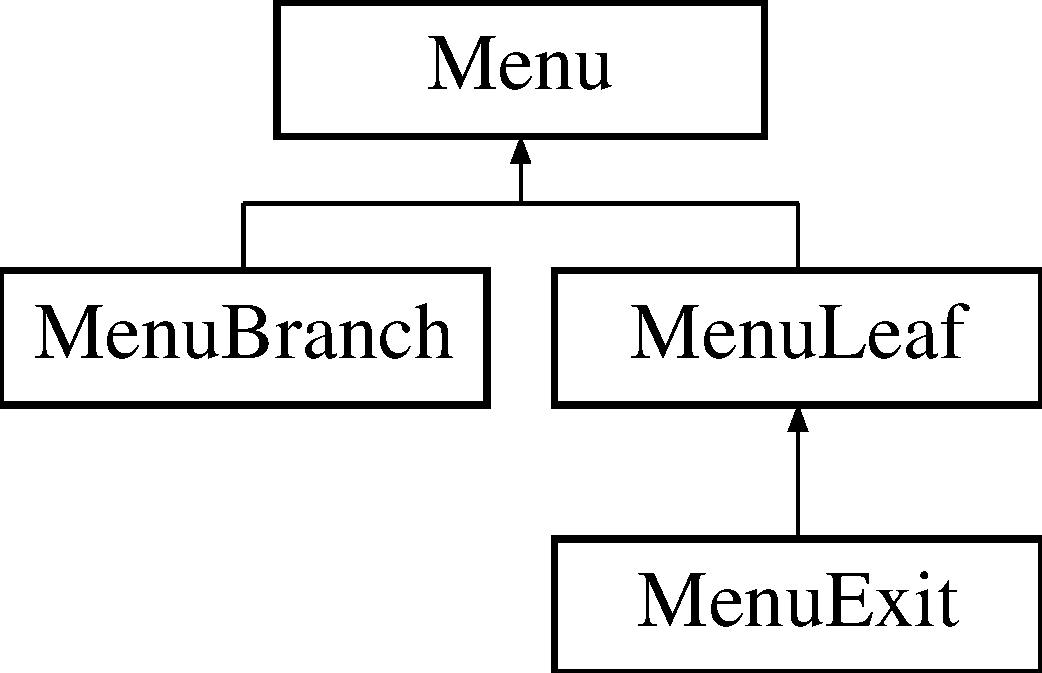
\includegraphics[height=3.000000cm]{class_menu}
\end{center}
\end{figure}
\subsection*{Public Member Functions}
\begin{DoxyCompactItemize}
\item 
\hypertarget{class_menu_a7da7bee39912b38ada59667090c95d45}{}{\bfseries Menu} (std\+::string title, \hyperlink{class_menu}{Menu} $\ast$sub\+\_\+menu)\label{class_menu_a7da7bee39912b38ada59667090c95d45}

\item 
\hypertarget{class_menu_a3baa9052815a249c1e149a7040bcd4ca}{}\hyperlink{class_menu}{Menu} $\ast$ {\bfseries add} (std\+::string title, \hyperlink{class_menu}{Menu} $\ast$sub\+\_\+menu)\label{class_menu_a3baa9052815a249c1e149a7040bcd4ca}

\item 
\hypertarget{class_menu_a4bd9e81608d3fc5e7f1842b6987a1f04}{}std\+::vector$<$ std\+::string $>$ {\bfseries get\+Menu} ()\label{class_menu_a4bd9e81608d3fc5e7f1842b6987a1f04}

\item 
\hypertarget{class_menu_ae29e1187192f79766d1ccfad7e757381}{}\hyperlink{class_menu}{Menu} $\ast$ {\bfseries get\+Parent} ()\label{class_menu_ae29e1187192f79766d1ccfad7e757381}

\item 
\hypertarget{class_menu_ae742121ce17557526642251a67f32dd0}{}virtual \hyperlink{class_menu}{Menu} $\ast$ {\bfseries action} (std\+::string input)=0\label{class_menu_ae742121ce17557526642251a67f32dd0}

\end{DoxyCompactItemize}
\subsection*{Protected Attributes}
\begin{DoxyCompactItemize}
\item 
\hypertarget{class_menu_a80c14bde1c02ea015233b942ce81bdaa}{}\hyperlink{class_menu}{Menu} $\ast$ {\bfseries parent} = nullptr\label{class_menu_a80c14bde1c02ea015233b942ce81bdaa}

\item 
\hypertarget{class_menu_abb38f232d59205161dd37d752f881bb2}{}std\+::vector$<$ std\+::pair$<$ std\+::string, \hyperlink{class_menu}{Menu} $\ast$ $>$ $>$ {\bfseries menu}\label{class_menu_abb38f232d59205161dd37d752f881bb2}

\end{DoxyCompactItemize}


The documentation for this class was generated from the following files\+:\begin{DoxyCompactItemize}
\item 
D\+:/\+Users/\+Gregory/\+One\+Drive/\+Git\+Hub/\+Icon\+Magic/\+Source/main/\+Menu/Menu.\+hpp\item 
D\+:/\+Users/\+Gregory/\+One\+Drive/\+Git\+Hub/\+Icon\+Magic/\+Source/main/\+Menu/Menu.\+cpp\end{DoxyCompactItemize}

\hypertarget{class_menu_branch}{}\section{Menu\+Branch Class Reference}
\label{class_menu_branch}\index{Menu\+Branch@{Menu\+Branch}}
Inheritance diagram for Menu\+Branch\+:\begin{figure}[H]
\begin{center}
\leavevmode
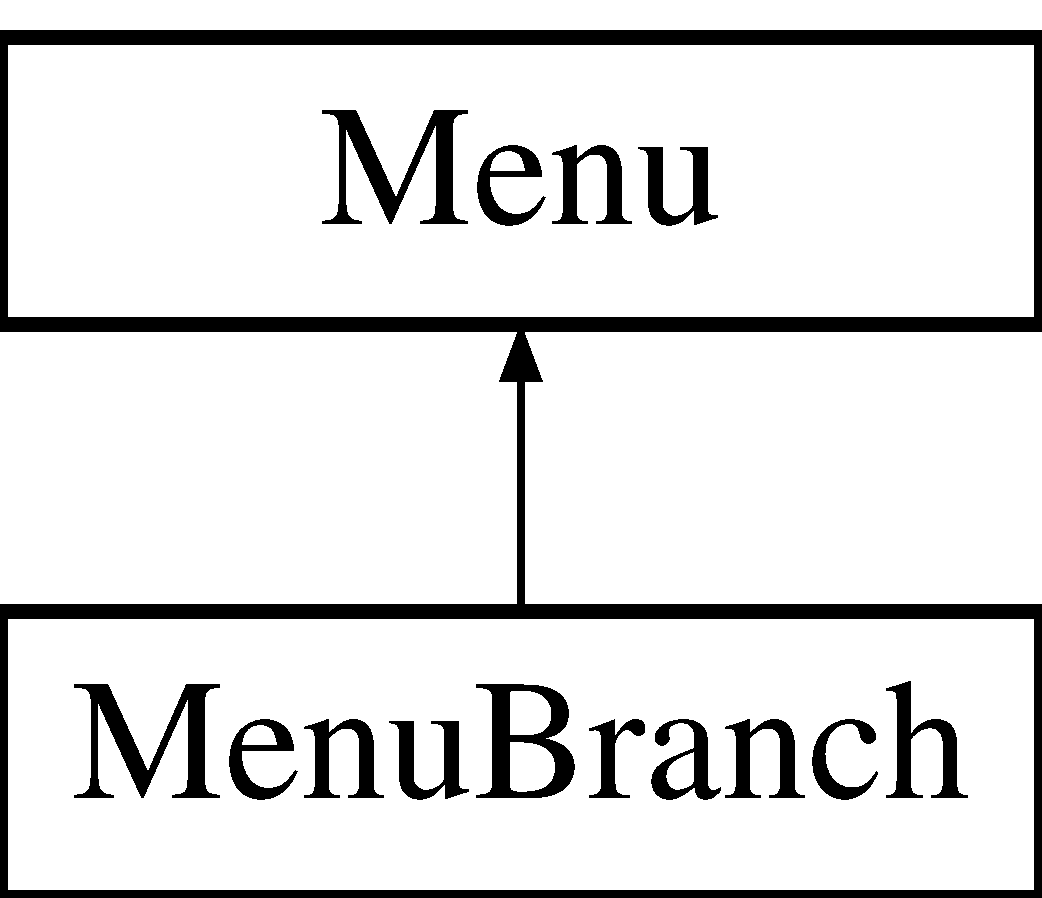
\includegraphics[height=2.000000cm]{class_menu_branch}
\end{center}
\end{figure}
\subsection*{Public Member Functions}
\begin{DoxyCompactItemize}
\item 
\hypertarget{class_menu_branch_aed402cc6b56fc8721b7901337b8bcf4c}{}\hyperlink{class_menu}{Menu} $\ast$ {\bfseries action} (std\+::string input)\label{class_menu_branch_aed402cc6b56fc8721b7901337b8bcf4c}

\end{DoxyCompactItemize}
\subsection*{Additional Inherited Members}


The documentation for this class was generated from the following files\+:\begin{DoxyCompactItemize}
\item 
D\+:/\+Users/\+Gregory/\+One\+Drive/\+Git\+Hub/\+Icon\+Magic/\+Source/main/\+Menu/Menu.\+hpp\item 
D\+:/\+Users/\+Gregory/\+One\+Drive/\+Git\+Hub/\+Icon\+Magic/\+Source/main/\+Menu/Menu.\+cpp\end{DoxyCompactItemize}

\hypertarget{class_menu_exit}{}\section{Menu\+Exit Class Reference}
\label{class_menu_exit}\index{Menu\+Exit@{Menu\+Exit}}
Inheritance diagram for Menu\+Exit\+:\begin{figure}[H]
\begin{center}
\leavevmode
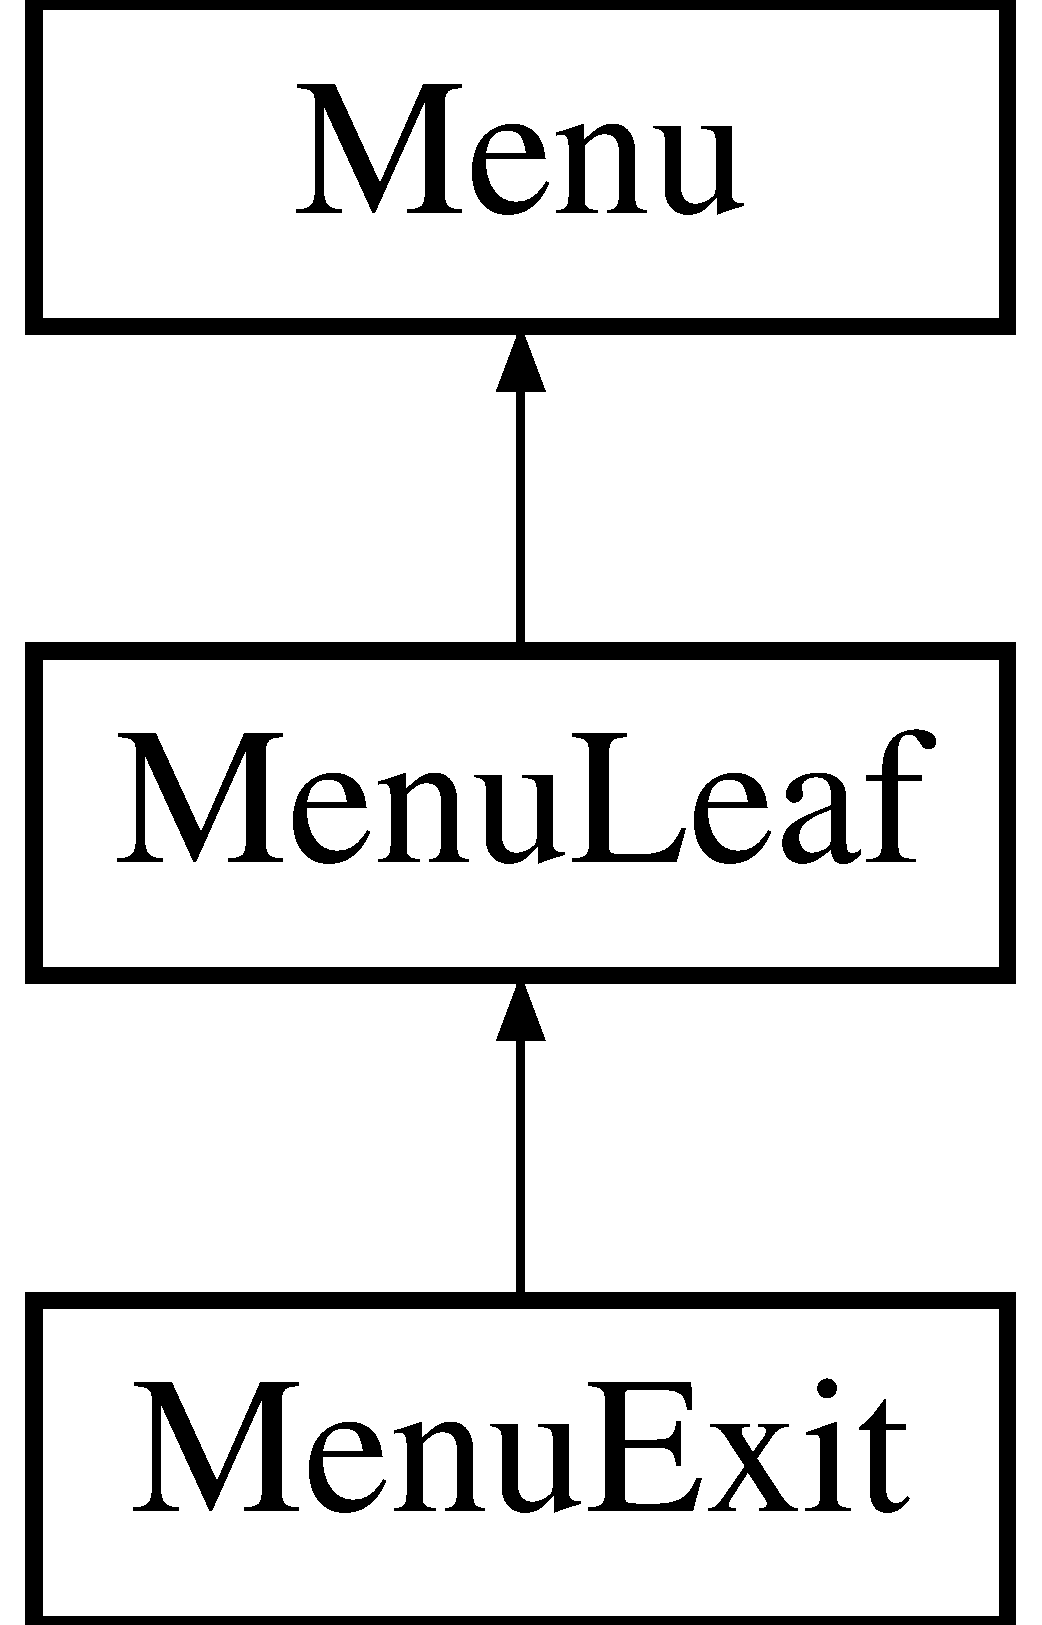
\includegraphics[height=3.000000cm]{class_menu_exit}
\end{center}
\end{figure}
\subsection*{Public Member Functions}
\begin{DoxyCompactItemize}
\item 
\hypertarget{class_menu_exit_aa926e3f17919a4b35f703ad926de4e07}{}\hyperlink{class_menu}{Menu} $\ast$ {\bfseries action} (std\+::string \+\_\+)\label{class_menu_exit_aa926e3f17919a4b35f703ad926de4e07}

\end{DoxyCompactItemize}
\subsection*{Additional Inherited Members}


The documentation for this class was generated from the following files\+:\begin{DoxyCompactItemize}
\item 
D\+:/\+Users/\+Gregory/\+One\+Drive/\+Git\+Hub/\+Icon\+Magic/\+Source/main/\+Menu/Menu.\+hpp\item 
D\+:/\+Users/\+Gregory/\+One\+Drive/\+Git\+Hub/\+Icon\+Magic/\+Source/main/\+Menu/Menu.\+cpp\end{DoxyCompactItemize}

\hypertarget{class_menu_factory}{}\section{Menu\+Factory Class Reference}
\label{class_menu_factory}\index{Menu\+Factory@{Menu\+Factory}}
\subsection*{Public Member Functions}
\begin{DoxyCompactItemize}
\item 
\hypertarget{class_menu_factory_a7741d0ab75b28c6a8374f4cb0adf9872}{}\hyperlink{class_menu}{Menu} $\ast$ {\bfseries get\+Main\+Menu\+Instance} ()\label{class_menu_factory_a7741d0ab75b28c6a8374f4cb0adf9872}

\end{DoxyCompactItemize}


The documentation for this class was generated from the following files\+:\begin{DoxyCompactItemize}
\item 
D\+:/\+Users/\+Gregory/\+One\+Drive/\+Git\+Hub/\+Icon\+Magic/\+Source/main/\+Menu/\+Menu\+Definitions/Menu\+Factory.\+hpp\item 
D\+:/\+Users/\+Gregory/\+One\+Drive/\+Git\+Hub/\+Icon\+Magic/\+Source/main/\+Menu/\+Menu\+Definitions/Menu\+Factory.\+cpp\end{DoxyCompactItemize}

\hypertarget{class_menu_leaf}{}\section{Menu\+Leaf Class Reference}
\label{class_menu_leaf}\index{Menu\+Leaf@{Menu\+Leaf}}
Inheritance diagram for Menu\+Leaf\+:\begin{figure}[H]
\begin{center}
\leavevmode
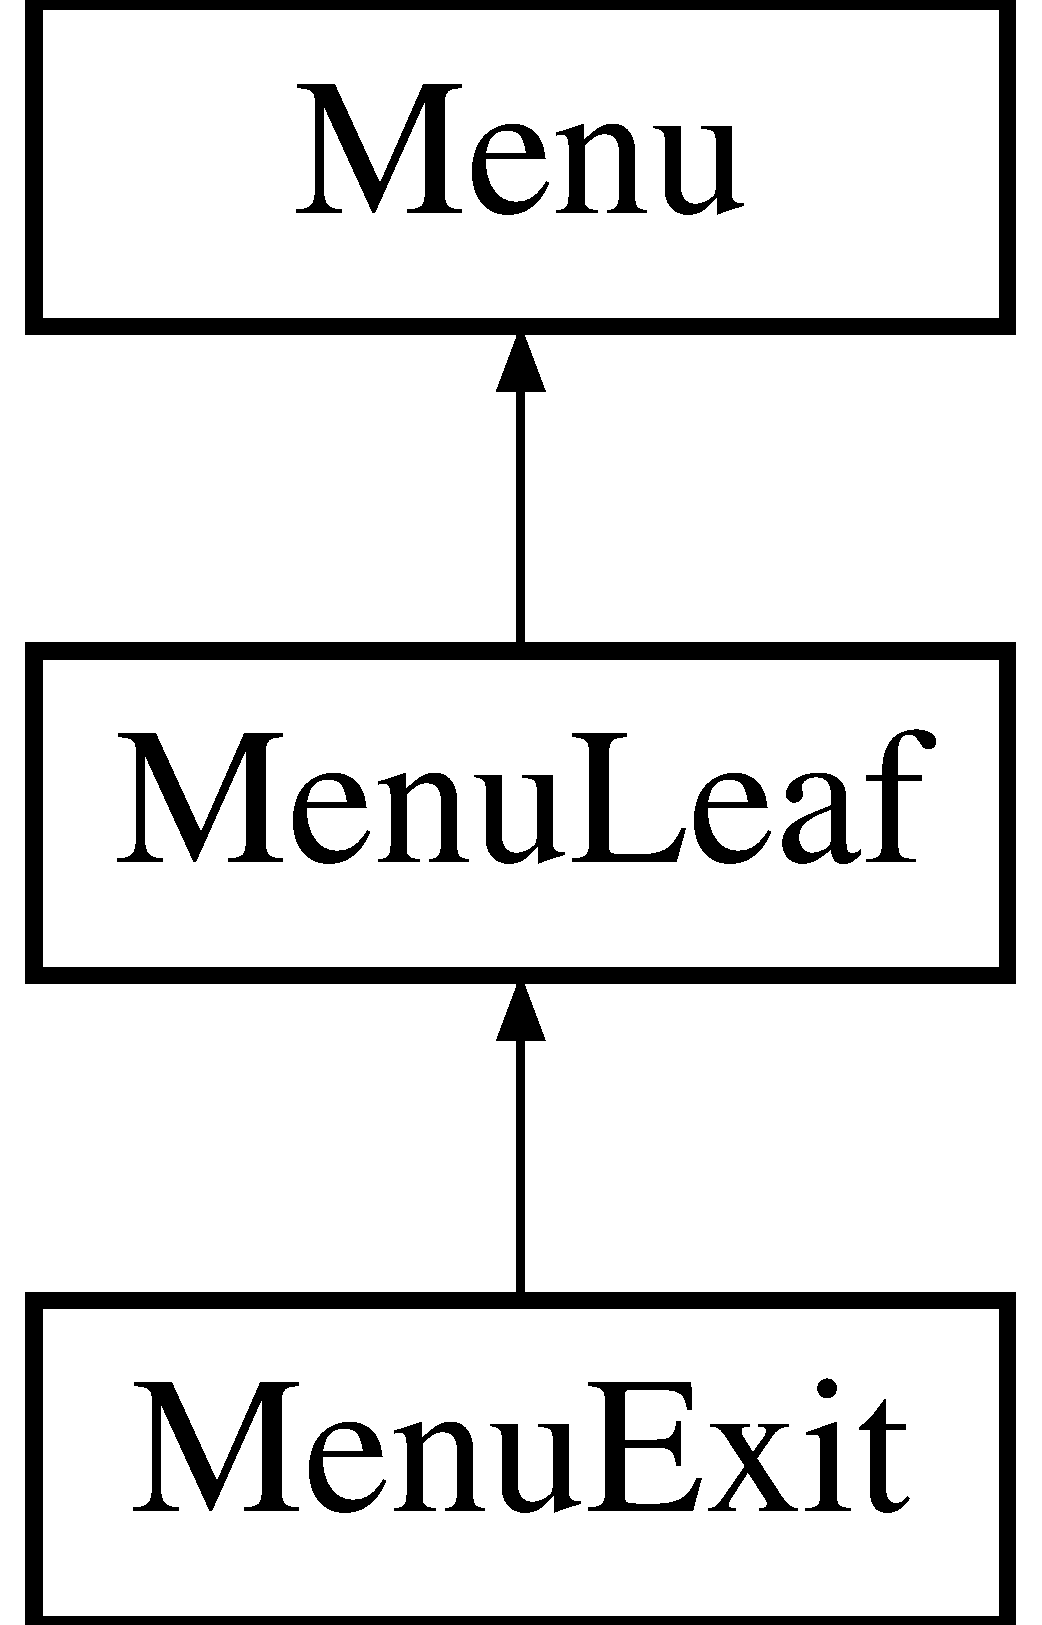
\includegraphics[height=3.000000cm]{class_menu_leaf}
\end{center}
\end{figure}
\subsection*{Public Member Functions}
\begin{DoxyCompactItemize}
\item 
\hypertarget{class_menu_leaf_a56748320ba902329a5c5dbe736f3a635}{}\hyperlink{class_menu}{Menu} $\ast$ {\bfseries action} (std\+::string input)\label{class_menu_leaf_a56748320ba902329a5c5dbe736f3a635}

\item 
\hypertarget{class_menu_leaf_a305d6b886a7c763d9e31b8196607d9a5}{}\hyperlink{class_menu}{Menu} $\ast$ {\bfseries add\+Action} (std\+::function$<$ int(void)$>$ f)\label{class_menu_leaf_a305d6b886a7c763d9e31b8196607d9a5}

\end{DoxyCompactItemize}
\subsection*{Additional Inherited Members}


The documentation for this class was generated from the following files\+:\begin{DoxyCompactItemize}
\item 
D\+:/\+Users/\+Gregory/\+One\+Drive/\+Git\+Hub/\+Icon\+Magic/\+Source/main/\+Menu/Menu.\+hpp\item 
D\+:/\+Users/\+Gregory/\+One\+Drive/\+Git\+Hub/\+Icon\+Magic/\+Source/main/\+Menu/Menu.\+cpp\end{DoxyCompactItemize}

\hypertarget{class_menu_manager}{}\section{Menu\+Manager Class Reference}
\label{class_menu_manager}\index{Menu\+Manager@{Menu\+Manager}}
\subsection*{Public Member Functions}
\begin{DoxyCompactItemize}
\item 
\hypertarget{class_menu_manager_a10697cb589a5f8e0192e9521435d0c67}{}{\bfseries Menu\+Manager} (\hyperlink{class_menu}{Menu} $\ast$menu\+\_\+handle)\label{class_menu_manager_a10697cb589a5f8e0192e9521435d0c67}

\item 
\hypertarget{class_menu_manager_ae6d30361fb03f8957d2e8e363ec0e4f3}{}void {\bfseries start} ()\label{class_menu_manager_ae6d30361fb03f8957d2e8e363ec0e4f3}

\end{DoxyCompactItemize}


The documentation for this class was generated from the following files\+:\begin{DoxyCompactItemize}
\item 
D\+:/\+Users/\+Gregory/\+One\+Drive/\+Git\+Hub/\+Icon\+Magic/\+Source/main/\+Menu/Menu\+Manager.\+hpp\item 
D\+:/\+Users/\+Gregory/\+One\+Drive/\+Git\+Hub/\+Icon\+Magic/\+Source/main/\+Menu/Menu\+Manager.\+cpp\end{DoxyCompactItemize}

\hypertarget{class_registry_access_exception}{}\section{Registry\+Access\+Exception Class Reference}
\label{class_registry_access_exception}\index{Registry\+Access\+Exception@{Registry\+Access\+Exception}}
Inheritance diagram for Registry\+Access\+Exception\+:\begin{figure}[H]
\begin{center}
\leavevmode
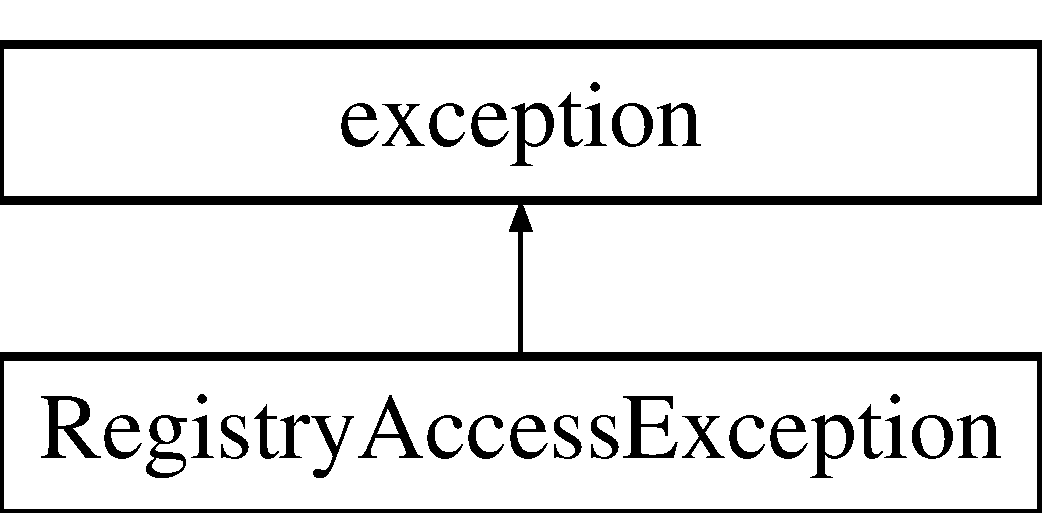
\includegraphics[height=2.000000cm]{class_registry_access_exception}
\end{center}
\end{figure}
\subsection*{Public Member Functions}
\begin{DoxyCompactItemize}
\item 
\hypertarget{class_registry_access_exception_a1a85d7c94398af682f3b29a022cce704}{}{\bfseries Registry\+Access\+Exception} (std\+::string message)\label{class_registry_access_exception_a1a85d7c94398af682f3b29a022cce704}

\item 
\hypertarget{class_registry_access_exception_a4306a07dd787c0f82e215bd0cb061e09}{}std\+::string {\bfseries what} ()\label{class_registry_access_exception_a4306a07dd787c0f82e215bd0cb061e09}

\end{DoxyCompactItemize}


The documentation for this class was generated from the following files\+:\begin{DoxyCompactItemize}
\item 
D\+:/\+Users/\+Gregory/\+One\+Drive/\+Git\+Hub/\+Icon\+Magic/\+Source/main/\+Registry/\+Data\+Access/Registry\+Access\+Exception.\+hpp\item 
D\+:/\+Users/\+Gregory/\+One\+Drive/\+Git\+Hub/\+Icon\+Magic/\+Source/main/\+Registry/\+Data\+Access/Registry\+Access\+Exception.\+cpp\end{DoxyCompactItemize}

\hypertarget{class_registry_history}{}\section{Registry\+History Class Reference}
\label{class_registry_history}\index{Registry\+History@{Registry\+History}}
\subsection*{Public Member Functions}
\begin{DoxyCompactItemize}
\item 
\hypertarget{class_registry_history_ab8ca406519bf9c2383af62b655e091ec}{}\hyperlink{class_registry_history_ab8ca406519bf9c2383af62b655e091ec}{Registry\+History} ()\label{class_registry_history_ab8ca406519bf9c2383af62b655e091ec}

\begin{DoxyCompactList}\small\item\em Default constructor. \end{DoxyCompactList}\item 
void \hyperlink{class_registry_history_afb10619d4c6e5b1eef4f27b11aa71ec8}{set\+History\+File\+Name} (std\+::string history\+\_\+file\+\_\+name)
\begin{DoxyCompactList}\small\item\em Set the path to the file to be used for storing registry modification history. \end{DoxyCompactList}\item 
bool \hyperlink{class_registry_history_a2a81ef9ef2d13fba16c4596a5e24409b}{read\+History} ()
\item 
bool \hyperlink{class_registry_history_ad05f552791c50a88291483544f9ffb80}{write\+History} ()
\item 
\hypertarget{class_registry_history_a3cad08c57fa9b967a9d7d2b1e7a672d1}{}bool {\bfseries push} (std\+::string extension\+\_\+name, std\+::string image\+\_\+name, std\+::string image\+\_\+index)\label{class_registry_history_a3cad08c57fa9b967a9d7d2b1e7a672d1}

\item 
\hypertarget{class_registry_history_a7dbf9ed9286304148a1e185d9642a994}{}bool {\bfseries pop} (std\+::string extension\+\_\+name)\label{class_registry_history_a7dbf9ed9286304148a1e185d9642a994}

\item 
\hypertarget{class_registry_history_a949045dc581267a6565c6f801ea2ddc2}{}void {\bfseries delete\+Extension} (std\+::string extension\+\_\+name)\label{class_registry_history_a949045dc581267a6565c6f801ea2ddc2}

\item 
\hypertarget{class_registry_history_af8cfe167195d0d5389f3a7dcc05b6b32}{}std\+::string {\bfseries get\+Path} (std\+::string extension\+\_\+name)\label{class_registry_history_af8cfe167195d0d5389f3a7dcc05b6b32}

\item 
\hypertarget{class_registry_history_a6abdebf855d10a0d914a9e02759b39bb}{}std\+::string {\bfseries get\+Index} (std\+::string extension\+\_\+name)\label{class_registry_history_a6abdebf855d10a0d914a9e02759b39bb}

\item 
\hypertarget{class_registry_history_ae941551e1a31a36fb0b37b0b6db6f224}{}std\+::string {\bfseries get\+Reg\+String} (std\+::string extension\+\_\+name)\label{class_registry_history_ae941551e1a31a36fb0b37b0b6db6f224}

\end{DoxyCompactItemize}


\subsection{Member Function Documentation}
\hypertarget{class_registry_history_a2a81ef9ef2d13fba16c4596a5e24409b}{}\index{Registry\+History@{Registry\+History}!read\+History@{read\+History}}
\index{read\+History@{read\+History}!Registry\+History@{Registry\+History}}
\subsubsection[{read\+History()}]{\setlength{\rightskip}{0pt plus 5cm}bool Registry\+History\+::read\+History (
\begin{DoxyParamCaption}
{}
\end{DoxyParamCaption}
)}\label{class_registry_history_a2a81ef9ef2d13fba16c4596a5e24409b}
\begin{DoxyReturn}{Returns}
bool 
\end{DoxyReturn}
\hypertarget{class_registry_history_afb10619d4c6e5b1eef4f27b11aa71ec8}{}\index{Registry\+History@{Registry\+History}!set\+History\+File\+Name@{set\+History\+File\+Name}}
\index{set\+History\+File\+Name@{set\+History\+File\+Name}!Registry\+History@{Registry\+History}}
\subsubsection[{set\+History\+File\+Name(std\+::string history\+\_\+file\+\_\+name)}]{\setlength{\rightskip}{0pt plus 5cm}void Registry\+History\+::set\+History\+File\+Name (
\begin{DoxyParamCaption}
\item[{std\+::string}]{history\+\_\+file\+\_\+name}
\end{DoxyParamCaption}
)}\label{class_registry_history_afb10619d4c6e5b1eef4f27b11aa71ec8}


Set the path to the file to be used for storing registry modification history. 


\begin{DoxyParams}{Parameters}
{\em history\+\_\+file\+\_\+name} & std\+::string \\
\hline
\end{DoxyParams}
\begin{DoxyReturn}{Returns}
void 
\end{DoxyReturn}
\hypertarget{class_registry_history_ad05f552791c50a88291483544f9ffb80}{}\index{Registry\+History@{Registry\+History}!write\+History@{write\+History}}
\index{write\+History@{write\+History}!Registry\+History@{Registry\+History}}
\subsubsection[{write\+History()}]{\setlength{\rightskip}{0pt plus 5cm}bool Registry\+History\+::write\+History (
\begin{DoxyParamCaption}
{}
\end{DoxyParamCaption}
)}\label{class_registry_history_ad05f552791c50a88291483544f9ffb80}
\begin{DoxyReturn}{Returns}
bool 
\end{DoxyReturn}


The documentation for this class was generated from the following files\+:\begin{DoxyCompactItemize}
\item 
D\+:/\+Users/\+Gregory/\+One\+Drive/\+Git\+Hub/\+Icon\+Magic/\+Source/main/\+Registry/\+History/Registry\+History.\+hpp\item 
D\+:/\+Users/\+Gregory/\+One\+Drive/\+Git\+Hub/\+Icon\+Magic/\+Source/main/\+Registry/\+History/\hyperlink{_registry_history_8cpp}{Registry\+History.\+cpp}\end{DoxyCompactItemize}

\hypertarget{class_registry_scan_exception}{}\section{Registry\+Scan\+Exception Class Reference}
\label{class_registry_scan_exception}\index{Registry\+Scan\+Exception@{Registry\+Scan\+Exception}}
Inheritance diagram for Registry\+Scan\+Exception\+:\begin{figure}[H]
\begin{center}
\leavevmode
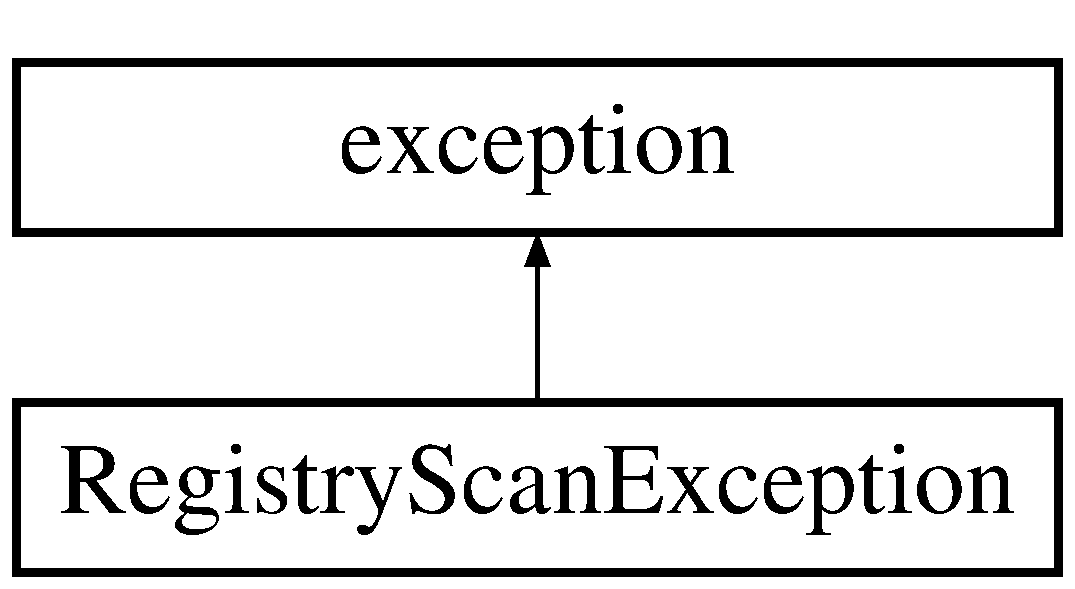
\includegraphics[height=2.000000cm]{class_registry_scan_exception}
\end{center}
\end{figure}
\subsection*{Public Member Functions}
\begin{DoxyCompactItemize}
\item 
\hypertarget{class_registry_scan_exception_a3fc3e488fa2ba4d314b4b925d4ecb623}{}{\bfseries Registry\+Scan\+Exception} (std\+::string msg)\label{class_registry_scan_exception_a3fc3e488fa2ba4d314b4b925d4ecb623}

\item 
\hypertarget{class_registry_scan_exception_afcc2a8528d6f0d8df61e716b4f166860}{}virtual const char $\ast$ {\bfseries what} () const   throw ()\label{class_registry_scan_exception_afcc2a8528d6f0d8df61e716b4f166860}

\end{DoxyCompactItemize}
\subsection*{Public Attributes}
\begin{DoxyCompactItemize}
\item 
\hypertarget{class_registry_scan_exception_a7aa8ae7d91676c28175bbe39f97c9515}{}std\+::string {\bfseries err} = \char`\"{}Unknown failure.\char`\"{}\label{class_registry_scan_exception_a7aa8ae7d91676c28175bbe39f97c9515}

\end{DoxyCompactItemize}


The documentation for this class was generated from the following file\+:\begin{DoxyCompactItemize}
\item 
D\+:/\+Users/\+Gregory/\+One\+Drive/\+Git\+Hub/\+Icon\+Magic/\+Source/main/\+Registry/\+Scanner/Scan\+Tool.\+hpp\end{DoxyCompactItemize}

\hypertarget{class_registry_scanner}{}\section{Registry\+Scanner Class Reference}
\label{class_registry_scanner}\index{Registry\+Scanner@{Registry\+Scanner}}
\subsection*{Public Member Functions}
\begin{DoxyCompactItemize}
\item 
\hypertarget{class_registry_scanner_a5a576a5caf8f03054ec1d66f97a507a3}{}std\+::vector$<$ std\+::pair$<$ \hyperlink{class_key_path}{Key\+Path}, std\+::string $>$ $>$ {\bfseries get\+Values} (std\+::string key\+\_\+name, std\+::string value\+\_\+name)\label{class_registry_scanner_a5a576a5caf8f03054ec1d66f97a507a3}

\item 
\hypertarget{class_registry_scanner_ab7a22643837934c1316038ac0fbd0f90}{}void {\bfseries set\+Root\+Key} (std\+::string root\+\_\+key\+\_\+name)\label{class_registry_scanner_ab7a22643837934c1316038ac0fbd0f90}

\item 
\hypertarget{class_registry_scanner_a5e934823c10e5d29ed223b5bc9c5145d}{}std\+::string {\bfseries get\+Root\+Key} ()\label{class_registry_scanner_a5e934823c10e5d29ed223b5bc9c5145d}

\item 
\hypertarget{class_registry_scanner_a31927ff653af4ae74d2bc8edd3c322f8}{}void {\bfseries set\+Max\+Depth} (int max\+\_\+depth)\label{class_registry_scanner_a31927ff653af4ae74d2bc8edd3c322f8}

\item 
\hypertarget{class_registry_scanner_aca1a71138cd3b330822bdf217407ead7}{}int {\bfseries get\+Max\+Depth} ()\label{class_registry_scanner_aca1a71138cd3b330822bdf217407ead7}

\item 
\hypertarget{class_registry_scanner_a0e456e336f9f6c1f4ab54b43754168ff}{}void {\bfseries set\+Max\+Matches} (int max\+\_\+matches)\label{class_registry_scanner_a0e456e336f9f6c1f4ab54b43754168ff}

\item 
\hypertarget{class_registry_scanner_a3712b5c6cffd7b2c7426361124d63acc}{}int {\bfseries get\+Max\+Matches} ()\label{class_registry_scanner_a3712b5c6cffd7b2c7426361124d63acc}

\end{DoxyCompactItemize}
\subsection*{Static Public Member Functions}
\begin{DoxyCompactItemize}
\item 
\hypertarget{class_registry_scanner_a53c683cba9076bbe56eebc18b140c0c3}{}static int {\bfseries unlimited\+Matches} ()\label{class_registry_scanner_a53c683cba9076bbe56eebc18b140c0c3}

\item 
\hypertarget{class_registry_scanner_a97303e1189cc7a6982aa7484d929f966}{}static int {\bfseries unlimited\+Recursion\+Depth} ()\label{class_registry_scanner_a97303e1189cc7a6982aa7484d929f966}

\end{DoxyCompactItemize}


The documentation for this class was generated from the following files\+:\begin{DoxyCompactItemize}
\item 
D\+:/\+Users/\+Gregory/\+One\+Drive/\+Git\+Hub/\+Icon\+Magic/\+Source/main/\+Registry/\+Scanner/Registry\+Scanner.\+hpp\item 
D\+:/\+Users/\+Gregory/\+One\+Drive/\+Git\+Hub/\+Icon\+Magic/\+Source/main/\+Registry/\+Scanner/Registry\+Scanner.\+cpp\end{DoxyCompactItemize}

\hypertarget{class_scan_tool}{}\section{Scan\+Tool Class Reference}
\label{class_scan_tool}\index{Scan\+Tool@{Scan\+Tool}}
\subsection*{Public Member Functions}
\begin{DoxyCompactItemize}
\item 
\hypertarget{class_scan_tool_acc6643d8c5a139801f0a3ab33a4fd64b}{}std\+::vector$<$ std\+::pair$<$ \hyperlink{class_key_path}{Key\+Path}, std\+::string $>$ $>$ {\bfseries simple\+Search} (std\+::string root\+\_\+key\+\_\+name, std\+::string search\+\_\+key\+\_\+name, std\+::string search\+\_\+value\+\_\+name, int maximum\+\_\+recursion\+\_\+depth, int maximum\+\_\+items\+\_\+to\+\_\+search\+\_\+for)\label{class_scan_tool_acc6643d8c5a139801f0a3ab33a4fd64b}

\item 
\hypertarget{class_scan_tool_a1fd28a95d2d3d088fcc40ba1d4d886c5}{}bool {\bfseries test\+Root\+Key\+Name\+Valid} (std\+::string root\+\_\+key\+\_\+name)\label{class_scan_tool_a1fd28a95d2d3d088fcc40ba1d4d886c5}

\end{DoxyCompactItemize}
\subsection*{Static Public Member Functions}
\begin{DoxyCompactItemize}
\item 
\hypertarget{class_scan_tool_a40991a4b76a30662a9e9c3bd54aae071}{}static int {\bfseries unlimited\+Matches} ()\label{class_scan_tool_a40991a4b76a30662a9e9c3bd54aae071}

\item 
\hypertarget{class_scan_tool_ae4c8ee31af682ac9ec0fce9e861b38eb}{}static int {\bfseries unlimited\+Recursion\+Depth} ()\label{class_scan_tool_ae4c8ee31af682ac9ec0fce9e861b38eb}

\end{DoxyCompactItemize}
\subsection*{Static Public Attributes}
\begin{DoxyCompactItemize}
\item 
\hypertarget{class_scan_tool_aeb6d958e5b7465c2e6cf871928bf3868}{}static const int {\bfseries U\+N\+L\+I\+M\+I\+T\+E\+D\+\_\+\+R\+E\+C\+U\+R\+S\+I\+O\+N\+\_\+\+D\+E\+P\+T\+H} = -\/7\label{class_scan_tool_aeb6d958e5b7465c2e6cf871928bf3868}

\item 
\hypertarget{class_scan_tool_a9a62696f3cd27f7cbec7fb9c27b7b1ba}{}static const int {\bfseries U\+N\+L\+I\+M\+I\+T\+E\+D\+\_\+\+M\+A\+T\+C\+H\+E\+S} = -\/7\label{class_scan_tool_a9a62696f3cd27f7cbec7fb9c27b7b1ba}

\end{DoxyCompactItemize}


The documentation for this class was generated from the following files\+:\begin{DoxyCompactItemize}
\item 
D\+:/\+Users/\+Gregory/\+One\+Drive/\+Git\+Hub/\+Icon\+Magic/\+Source/main/\+Registry/\+Scanner/Scan\+Tool.\+hpp\item 
D\+:/\+Users/\+Gregory/\+One\+Drive/\+Git\+Hub/\+Icon\+Magic/\+Source/main/\+Registry/\+Scanner/Scan\+Tool.\+cpp\end{DoxyCompactItemize}

\hypertarget{class_simple_registry_access}{}\section{Simple\+Registry\+Access Class Reference}
\label{class_simple_registry_access}\index{Simple\+Registry\+Access@{Simple\+Registry\+Access}}
\subsection*{Static Public Member Functions}
\begin{DoxyCompactItemize}
\item 
\hypertarget{class_simple_registry_access_accef2c679695c6e05a9e7c1c2a962481}{}static std\+::string {\bfseries get\+Value\+At\+Path} (\hyperlink{class_key_path}{Key\+Path} key\+\_\+path, std\+::string value\+\_\+name)\label{class_simple_registry_access_accef2c679695c6e05a9e7c1c2a962481}

\item 
\hypertarget{class_simple_registry_access_afb4986051b99ff89e156a2ab6b89aca3}{}static std\+::string {\bfseries get\+Value\+At\+Path} (\hyperlink{class_key_path}{Key\+Path} key\+\_\+path)\label{class_simple_registry_access_afb4986051b99ff89e156a2ab6b89aca3}

\item 
\hypertarget{class_simple_registry_access_a75e85e4de87a14c50a81b3cd080a2a97}{}static bool {\bfseries set\+Value\+At\+Path} (\hyperlink{class_key_path}{Key\+Path} key\+\_\+path, std\+::string value\+\_\+name, std\+::string value)\label{class_simple_registry_access_a75e85e4de87a14c50a81b3cd080a2a97}

\item 
\hypertarget{class_simple_registry_access_aea8420eb295c6c9e11093b1928a8591c}{}static bool {\bfseries set\+Value\+At\+Path} (\hyperlink{class_key_path}{Key\+Path} key\+\_\+path, std\+::string value)\label{class_simple_registry_access_aea8420eb295c6c9e11093b1928a8591c}

\end{DoxyCompactItemize}


The documentation for this class was generated from the following files\+:\begin{DoxyCompactItemize}
\item 
D\+:/\+Users/\+Gregory/\+One\+Drive/\+Git\+Hub/\+Icon\+Magic/\+Source/main/\+Registry/\+Data\+Access/Simple\+Registry\+Access.\+hpp\item 
D\+:/\+Users/\+Gregory/\+One\+Drive/\+Git\+Hub/\+Icon\+Magic/\+Source/main/\+Registry/\+Data\+Access/Simple\+Registry\+Access.\+cpp\end{DoxyCompactItemize}

\hypertarget{class_test_framework}{}\section{Test\+Framework Class Reference}
\label{class_test_framework}\index{Test\+Framework@{Test\+Framework}}
\subsection*{Public Member Functions}
\begin{DoxyCompactItemize}
\item 
void \hyperlink{class_test_framework_a4f37e58d8b67f9da66372cf43f4281ae}{add\+Test} (std\+::function$<$ bool(void)$>$ test\+Function)
\begin{DoxyCompactList}\small\item\em add\+Test \end{DoxyCompactList}\item 
bool \hyperlink{class_test_framework_ace2588c0b0043546abc584b1d1b08e96}{execute} ()
\begin{DoxyCompactList}\small\item\em execute \end{DoxyCompactList}\item 
bool \hyperlink{class_test_framework_ae12aac94ee9a745eb3ce46f5d003dcf2}{get\+Tests\+Status} ()
\begin{DoxyCompactList}\small\item\em get\+Test\+Status \end{DoxyCompactList}\item 
int \hyperlink{class_test_framework_ad35b7b750378155531cf65e8163b67dd}{get\+Total\+Tests\+Run} ()
\begin{DoxyCompactList}\small\item\em get\+Total\+Tests\+Run \end{DoxyCompactList}\item 
int \hyperlink{class_test_framework_a34508c693cf7a3be01a3975065fa2457}{get\+Total\+Tests\+Run\+Successfully} ()
\begin{DoxyCompactList}\small\item\em get\+Total\+Tests\+Run\+Successfully \end{DoxyCompactList}\item 
\hyperlink{class_test_framework_a80e30a085718a9e3db4e6f4e79cc9d48}{Test\+Framework} ()
\begin{DoxyCompactList}\small\item\em \hyperlink{class_test_framework}{Test\+Framework}. \end{DoxyCompactList}\item 
\hyperlink{class_test_framework_aad3d6888fe40a083e767061a1ebf0c1d}{$\sim$\+Test\+Framework} ()
\begin{DoxyCompactList}\small\item\em $\sim$\+Test\+Framework \end{DoxyCompactList}\end{DoxyCompactItemize}


\subsection{Constructor \& Destructor Documentation}
\hypertarget{class_test_framework_a80e30a085718a9e3db4e6f4e79cc9d48}{}\index{Test\+Framework@{Test\+Framework}!Test\+Framework@{Test\+Framework}}
\index{Test\+Framework@{Test\+Framework}!Test\+Framework@{Test\+Framework}}
\subsubsection[{Test\+Framework()}]{\setlength{\rightskip}{0pt plus 5cm}Test\+Framework\+::\+Test\+Framework (
\begin{DoxyParamCaption}
{}
\end{DoxyParamCaption}
)}\label{class_test_framework_a80e30a085718a9e3db4e6f4e79cc9d48}


\hyperlink{class_test_framework}{Test\+Framework}. 

\begin{DoxyRefDesc}{Todo}
\item[\hyperlink{todo__todo000006}{Todo}]\+: document this function \end{DoxyRefDesc}
\hypertarget{class_test_framework_aad3d6888fe40a083e767061a1ebf0c1d}{}\index{Test\+Framework@{Test\+Framework}!````~Test\+Framework@{$\sim$\+Test\+Framework}}
\index{````~Test\+Framework@{$\sim$\+Test\+Framework}!Test\+Framework@{Test\+Framework}}
\subsubsection[{$\sim$\+Test\+Framework()}]{\setlength{\rightskip}{0pt plus 5cm}Test\+Framework\+::$\sim$\+Test\+Framework (
\begin{DoxyParamCaption}
{}
\end{DoxyParamCaption}
)}\label{class_test_framework_aad3d6888fe40a083e767061a1ebf0c1d}


$\sim$\+Test\+Framework 

\begin{DoxyRefDesc}{Todo}
\item[\hyperlink{todo__todo000007}{Todo}]\+: document this function \end{DoxyRefDesc}


\subsection{Member Function Documentation}
\hypertarget{class_test_framework_a4f37e58d8b67f9da66372cf43f4281ae}{}\index{Test\+Framework@{Test\+Framework}!add\+Test@{add\+Test}}
\index{add\+Test@{add\+Test}!Test\+Framework@{Test\+Framework}}
\subsubsection[{add\+Test(std\+::function$<$ bool(void)$>$ test\+Function)}]{\setlength{\rightskip}{0pt plus 5cm}void Test\+Framework\+::add\+Test (
\begin{DoxyParamCaption}
\item[{std\+::function$<$ bool(void)$>$}]{test\+Function}
\end{DoxyParamCaption}
)}\label{class_test_framework_a4f37e58d8b67f9da66372cf43f4281ae}


add\+Test 

\begin{DoxyRefDesc}{Todo}
\item[\hyperlink{todo__todo000001}{Todo}]\+: document this function \end{DoxyRefDesc}
\hypertarget{class_test_framework_ace2588c0b0043546abc584b1d1b08e96}{}\index{Test\+Framework@{Test\+Framework}!execute@{execute}}
\index{execute@{execute}!Test\+Framework@{Test\+Framework}}
\subsubsection[{execute()}]{\setlength{\rightskip}{0pt plus 5cm}bool Test\+Framework\+::execute (
\begin{DoxyParamCaption}
{}
\end{DoxyParamCaption}
)}\label{class_test_framework_ace2588c0b0043546abc584b1d1b08e96}


execute 

\begin{DoxyRefDesc}{Todo}
\item[\hyperlink{todo__todo000002}{Todo}]\+: document this function \end{DoxyRefDesc}
\hypertarget{class_test_framework_ae12aac94ee9a745eb3ce46f5d003dcf2}{}\index{Test\+Framework@{Test\+Framework}!get\+Tests\+Status@{get\+Tests\+Status}}
\index{get\+Tests\+Status@{get\+Tests\+Status}!Test\+Framework@{Test\+Framework}}
\subsubsection[{get\+Tests\+Status()}]{\setlength{\rightskip}{0pt plus 5cm}bool Test\+Framework\+::get\+Tests\+Status (
\begin{DoxyParamCaption}
{}
\end{DoxyParamCaption}
)}\label{class_test_framework_ae12aac94ee9a745eb3ce46f5d003dcf2}


get\+Test\+Status 

\begin{DoxyRefDesc}{Todo}
\item[\hyperlink{todo__todo000003}{Todo}]\+: document this function \end{DoxyRefDesc}
\hypertarget{class_test_framework_ad35b7b750378155531cf65e8163b67dd}{}\index{Test\+Framework@{Test\+Framework}!get\+Total\+Tests\+Run@{get\+Total\+Tests\+Run}}
\index{get\+Total\+Tests\+Run@{get\+Total\+Tests\+Run}!Test\+Framework@{Test\+Framework}}
\subsubsection[{get\+Total\+Tests\+Run()}]{\setlength{\rightskip}{0pt plus 5cm}int Test\+Framework\+::get\+Total\+Tests\+Run (
\begin{DoxyParamCaption}
{}
\end{DoxyParamCaption}
)}\label{class_test_framework_ad35b7b750378155531cf65e8163b67dd}


get\+Total\+Tests\+Run 

\begin{DoxyRefDesc}{Todo}
\item[\hyperlink{todo__todo000004}{Todo}]\+: document this function \end{DoxyRefDesc}
\hypertarget{class_test_framework_a34508c693cf7a3be01a3975065fa2457}{}\index{Test\+Framework@{Test\+Framework}!get\+Total\+Tests\+Run\+Successfully@{get\+Total\+Tests\+Run\+Successfully}}
\index{get\+Total\+Tests\+Run\+Successfully@{get\+Total\+Tests\+Run\+Successfully}!Test\+Framework@{Test\+Framework}}
\subsubsection[{get\+Total\+Tests\+Run\+Successfully()}]{\setlength{\rightskip}{0pt plus 5cm}int Test\+Framework\+::get\+Total\+Tests\+Run\+Successfully (
\begin{DoxyParamCaption}
{}
\end{DoxyParamCaption}
)}\label{class_test_framework_a34508c693cf7a3be01a3975065fa2457}


get\+Total\+Tests\+Run\+Successfully 

\begin{DoxyRefDesc}{Todo}
\item[\hyperlink{todo__todo000005}{Todo}]\+: document this function \end{DoxyRefDesc}


The documentation for this class was generated from the following files\+:\begin{DoxyCompactItemize}
\item 
D\+:/\+Users/\+Gregory/\+One\+Drive/\+Git\+Hub/\+Icon\+Magic/\+Source/test/framework.\+hpp\item 
D\+:/\+Users/\+Gregory/\+One\+Drive/\+Git\+Hub/\+Icon\+Magic/\+Source/test/\hyperlink{framework_8cpp}{framework.\+cpp}\end{DoxyCompactItemize}

\chapter{File Documentation}
\hypertarget{example_8hpp}{}\section{D\+:/\+Users/\+Gregory/\+One\+Drive/\+Git\+Hub/\+Icon\+Magic/\+Source/doxygen/example.hpp File Reference}
\label{example_8hpp}\index{D\+:/\+Users/\+Gregory/\+One\+Drive/\+Git\+Hub/\+Icon\+Magic/\+Source/doxygen/example.\+hpp@{D\+:/\+Users/\+Gregory/\+One\+Drive/\+Git\+Hub/\+Icon\+Magic/\+Source/doxygen/example.\+hpp}}


Examples of the doxygen markup I plan to use accross the project.  


\subsection*{Classes}
\begin{DoxyCompactItemize}
\item 
class \hyperlink{class_example_class}{Example\+Class}
\begin{DoxyCompactList}\small\item\em An example class. \end{DoxyCompactList}\end{DoxyCompactItemize}


\subsection{Detailed Description}
Examples of the doxygen markup I plan to use accross the project. 

Given that I\textquotesingle{}m new to using doxygen, I thought it\textquotesingle{}d be a good idea to get to know it\textquotesingle{}s capabilaties in a sandbox rather than documenting everything then changing my mind over and over again and having to redo very bit of documentation every time.

You can use the folowwing to document items, hopefully obviously -\/ struct, union, enum, fn, var, def, typedef, file, namespace 
\hypertarget{main_8cpp}{}\section{D\+:/\+Users/\+Gregory/\+One\+Drive/\+Git\+Hub/\+Icon\+Magic/\+Source/main.cpp File Reference}
\label{main_8cpp}\index{D\+:/\+Users/\+Gregory/\+One\+Drive/\+Git\+Hub/\+Icon\+Magic/\+Source/main.\+cpp@{D\+:/\+Users/\+Gregory/\+One\+Drive/\+Git\+Hub/\+Icon\+Magic/\+Source/main.\+cpp}}


Created by Theta\+Sinner (Gregory Jensen). Released as open source.  


{\ttfamily \#include \char`\"{}main/\+Icon\+Magic.\+hpp\char`\"{}}\\*
{\ttfamily \#include $<$iostream$>$}\\*
{\ttfamily \#include \char`\"{}./main/\+Registry/\+Scanner/\+Scan\+Tool.\+hpp\char`\"{}}\\*
{\ttfamily \#include \char`\"{}./main/\+Registry/\+Data\+Access/\+Simple\+Registry\+Access.\+hpp\char`\"{}}\\*
{\ttfamily \#include $<$sstream$>$}\\*
{\ttfamily \#include $<$fstream$>$}\\*
{\ttfamily \#include $<$list$>$}\\*
{\ttfamily \#include $<$string$>$}\\*
{\ttfamily \#include \char`\"{}./main/\+Menu/\+Menu.\+hpp\char`\"{}}\\*
{\ttfamily \#include \char`\"{}./main/\+Menu/\+Menu\+Manager.\+hpp\char`\"{}}\\*
{\ttfamily \#include \char`\"{}./main/\+Menu/\+Menu\+Definitions/\+Menu\+Factory.\+hpp\char`\"{}}\\*
{\ttfamily \#include \char`\"{}./main/\+Manager.\+hpp\char`\"{}}\\*
{\ttfamily \#include \char`\"{}./main/\+Util.\+hpp\char`\"{}}\\*
\subsection*{Functions}
\begin{DoxyCompactItemize}
\item 
\hypertarget{main_8cpp_a7a29781a20c5dd4153c3c1cecf0ff328}{}int {\bfseries main} (int argc, char $\ast$$\ast$args)\label{main_8cpp_a7a29781a20c5dd4153c3c1cecf0ff328}

\end{DoxyCompactItemize}


\subsection{Detailed Description}
Created by Theta\+Sinner (Gregory Jensen). Released as open source. 

This file launches Icon\+Magic. 
\hypertarget{_icon_magic_8cpp}{}\section{D\+:/\+Users/\+Gregory/\+One\+Drive/\+Git\+Hub/\+Icon\+Magic/\+Source/\+Icon\+Magic.cpp File Reference}
\label{_icon_magic_8cpp}\index{D\+:/\+Users/\+Gregory/\+One\+Drive/\+Git\+Hub/\+Icon\+Magic/\+Source/\+Icon\+Magic.\+cpp@{D\+:/\+Users/\+Gregory/\+One\+Drive/\+Git\+Hub/\+Icon\+Magic/\+Source/\+Icon\+Magic.\+cpp}}


Created by Theta\+Sinner (Gregory Jensen). Released as open source.  


{\ttfamily \#include \char`\"{}Icon\+Magic.\+hpp\char`\"{}}\\*
\subsection*{Functions}
\begin{DoxyCompactItemize}
\item 
\hypertarget{_icon_magic_8cpp_ab447eac5ecb3b16e6d1aa9c4207c7443}{}int {\bfseries exit\+Icon\+Magic} (int exit\+Code=0)\label{_icon_magic_8cpp_ab447eac5ecb3b16e6d1aa9c4207c7443}

\item 
\hypertarget{_icon_magic_8cpp_a7e77140d7207e9d2e57821eb4547c175}{}int {\bfseries run\+Icon\+Magic} ()\label{_icon_magic_8cpp_a7e77140d7207e9d2e57821eb4547c175}

\end{DoxyCompactItemize}


\subsection{Detailed Description}
Created by Theta\+Sinner (Gregory Jensen). Released as open source. 

// T\+O\+D\+O file\+\_\+desc 
\hypertarget{_icon_magic_8hpp}{}\section{D\+:/\+Users/\+Gregory/\+One\+Drive/\+Git\+Hub/\+Icon\+Magic/\+Source/\+Icon\+Magic.hpp File Reference}
\label{_icon_magic_8hpp}\index{D\+:/\+Users/\+Gregory/\+One\+Drive/\+Git\+Hub/\+Icon\+Magic/\+Source/\+Icon\+Magic.\+hpp@{D\+:/\+Users/\+Gregory/\+One\+Drive/\+Git\+Hub/\+Icon\+Magic/\+Source/\+Icon\+Magic.\+hpp}}


Created by Theta\+Sinner (Gregory Jensen). Released as open source.  


{\ttfamily \#include $<$iostream$>$}\\*
{\ttfamily \#include $<$string$>$}\\*
{\ttfamily \#include $<$vector$>$}\\*
{\ttfamily \#include \char`\"{}System\+Validation.\+hpp\char`\"{}}\\*
{\ttfamily \#include \char`\"{}Windows\+Toolbox.\+hpp\char`\"{}}\\*
{\ttfamily \#include \char`\"{}Text\+U\+I.\+hpp\char`\"{}}\\*
\subsection*{Functions}
\begin{DoxyCompactItemize}
\item 
\hypertarget{_icon_magic_8hpp_a7e77140d7207e9d2e57821eb4547c175}{}int {\bfseries run\+Icon\+Magic} ()\label{_icon_magic_8hpp_a7e77140d7207e9d2e57821eb4547c175}

\end{DoxyCompactItemize}


\subsection{Detailed Description}
Created by Theta\+Sinner (Gregory Jensen). Released as open source. 

// T\+O\+D\+O file\+\_\+desc 
\hypertarget{_manager_8cpp}{}\section{D\+:/\+Users/\+Gregory/\+One\+Drive/\+Git\+Hub/\+Icon\+Magic/\+Source/main/\+Manager.cpp File Reference}
\label{_manager_8cpp}\index{D\+:/\+Users/\+Gregory/\+One\+Drive/\+Git\+Hub/\+Icon\+Magic/\+Source/main/\+Manager.\+cpp@{D\+:/\+Users/\+Gregory/\+One\+Drive/\+Git\+Hub/\+Icon\+Magic/\+Source/main/\+Manager.\+cpp}}


Created by Theta\+Sinner (Gregory Jensen). Released as open source.  


{\ttfamily \#include \char`\"{}./\+Manager.\+hpp\char`\"{}}\\*
{\ttfamily \#include $<$stdio.\+h$>$}\\*
{\ttfamily \#include \char`\"{}./\+Util.\+hpp\char`\"{}}\\*
{\ttfamily \#include \char`\"{}./\+Windows\+Toolbox.\+hpp\char`\"{}}\\*
{\ttfamily \#include \char`\"{}./\+Registry/\+Scanner/\+Registry\+Scanner.\+hpp\char`\"{}}\\*
{\ttfamily \#include \char`\"{}./\+Registry/\+History/registry\+History.\+hpp\char`\"{}}\\*


\subsection{Detailed Description}
Created by Theta\+Sinner (Gregory Jensen). Released as open source. 

// T\+O\+D\+O file\+\_\+desc 
\hypertarget{_manager_8hpp}{}\section{D\+:/\+Users/\+Gregory/\+One\+Drive/\+Git\+Hub/\+Icon\+Magic/\+Source/main/\+Manager.hpp File Reference}
\label{_manager_8hpp}\index{D\+:/\+Users/\+Gregory/\+One\+Drive/\+Git\+Hub/\+Icon\+Magic/\+Source/main/\+Manager.\+hpp@{D\+:/\+Users/\+Gregory/\+One\+Drive/\+Git\+Hub/\+Icon\+Magic/\+Source/main/\+Manager.\+hpp}}


Created by Theta\+Sinner (Gregory Jensen). Released as open source.  


{\ttfamily \#include $<$Windows.\+h$>$}\\*
{\ttfamily \#include $<$list$>$}\\*
{\ttfamily \#include $<$string$>$}\\*
{\ttfamily \#include $<$iostream$>$}\\*
{\ttfamily \#include $<$fstream$>$}\\*
\subsection*{Classes}
\begin{DoxyCompactItemize}
\item 
class \hyperlink{class_manager}{Manager}
\end{DoxyCompactItemize}


\subsection{Detailed Description}
Created by Theta\+Sinner (Gregory Jensen). Released as open source. 

// T\+O\+D\+O file\+\_\+desc 
\hypertarget{_key_path_8cpp}{}\section{D\+:/\+Users/\+Gregory/\+One\+Drive/\+Git\+Hub/\+Icon\+Magic/\+Source/main/\+Registry/\+Common/\+Key\+Path.cpp File Reference}
\label{_key_path_8cpp}\index{D\+:/\+Users/\+Gregory/\+One\+Drive/\+Git\+Hub/\+Icon\+Magic/\+Source/main/\+Registry/\+Common/\+Key\+Path.\+cpp@{D\+:/\+Users/\+Gregory/\+One\+Drive/\+Git\+Hub/\+Icon\+Magic/\+Source/main/\+Registry/\+Common/\+Key\+Path.\+cpp}}


The \hyperlink{class_key_path}{Key\+Path} class implementation.  


{\ttfamily \#include \char`\"{}./\+Key\+Path.\+hpp\char`\"{}}\\*


\subsection{Detailed Description}
The \hyperlink{class_key_path}{Key\+Path} class implementation. 

\begin{DoxySeeAlso}{See also}
\hyperlink{_key_path_8hpp}{Key\+Path.\+hpp} 
\end{DoxySeeAlso}

\hypertarget{_key_path_8hpp}{}\section{D\+:/\+Users/\+Gregory/\+One\+Drive/\+Git\+Hub/\+Icon\+Magic/\+Source/main/\+Registry/\+Common/\+Key\+Path.hpp File Reference}
\label{_key_path_8hpp}\index{D\+:/\+Users/\+Gregory/\+One\+Drive/\+Git\+Hub/\+Icon\+Magic/\+Source/main/\+Registry/\+Common/\+Key\+Path.\+hpp@{D\+:/\+Users/\+Gregory/\+One\+Drive/\+Git\+Hub/\+Icon\+Magic/\+Source/main/\+Registry/\+Common/\+Key\+Path.\+hpp}}


The \hyperlink{class_key_path}{Key\+Path} class definition.  


{\ttfamily \#include $<$vector$>$}\\*
{\ttfamily \#include $<$string$>$}\\*
\subsection*{Classes}
\begin{DoxyCompactItemize}
\item 
class \hyperlink{class_key_path}{Key\+Path}
\begin{DoxyCompactList}\small\item\em Object representation of a registry path. \end{DoxyCompactList}\end{DoxyCompactItemize}


\subsection{Detailed Description}
The \hyperlink{class_key_path}{Key\+Path} class definition. 

\begin{DoxySeeAlso}{See also}
\hyperlink{_key_path_8cpp}{Key\+Path.\+cpp} 
\end{DoxySeeAlso}

\hypertarget{_key_service_8cpp}{}\section{D\+:/\+Users/\+Gregory/\+One\+Drive/\+Git\+Hub/\+Icon\+Magic/\+Source/main/\+Registry/\+Common/\+Key\+Service.cpp File Reference}
\label{_key_service_8cpp}\index{D\+:/\+Users/\+Gregory/\+One\+Drive/\+Git\+Hub/\+Icon\+Magic/\+Source/main/\+Registry/\+Common/\+Key\+Service.\+cpp@{D\+:/\+Users/\+Gregory/\+One\+Drive/\+Git\+Hub/\+Icon\+Magic/\+Source/main/\+Registry/\+Common/\+Key\+Service.\+cpp}}


The \hyperlink{class_key_service}{Key\+Service} class implementation.  


{\ttfamily \#include \char`\"{}./\+Key\+Service.\+hpp\char`\"{}}\\*


\subsection{Detailed Description}
The \hyperlink{class_key_service}{Key\+Service} class implementation. 

\begin{DoxySeeAlso}{See also}
\hyperlink{_key_service_8hpp}{Key\+Service.\+hpp} 
\end{DoxySeeAlso}

\hypertarget{_key_service_8hpp}{}\section{D\+:/\+Users/\+Gregory/\+One\+Drive/\+Git\+Hub/\+Icon\+Magic/\+Source/main/\+Registry/\+Common/\+Key\+Service.hpp File Reference}
\label{_key_service_8hpp}\index{D\+:/\+Users/\+Gregory/\+One\+Drive/\+Git\+Hub/\+Icon\+Magic/\+Source/main/\+Registry/\+Common/\+Key\+Service.\+hpp@{D\+:/\+Users/\+Gregory/\+One\+Drive/\+Git\+Hub/\+Icon\+Magic/\+Source/main/\+Registry/\+Common/\+Key\+Service.\+hpp}}


The \hyperlink{class_key_service}{Key\+Service} class definition.  


{\ttfamily \#include $<$Windows.\+h$>$}\\*
{\ttfamily \#include $<$string$>$}\\*
{\ttfamily \#include $<$map$>$}\\*
\subsection*{Classes}
\begin{DoxyCompactItemize}
\item 
class \hyperlink{class_key_service}{Key\+Service}
\begin{DoxyCompactList}\small\item\em Provides a key lookup service. \end{DoxyCompactList}\end{DoxyCompactItemize}


\subsection{Detailed Description}
The \hyperlink{class_key_service}{Key\+Service} class definition. 

\begin{DoxySeeAlso}{See also}
\hyperlink{_key_service_8cpp}{Key\+Service.\+cpp} 
\end{DoxySeeAlso}

\hypertarget{_direct_registry_access_8cpp}{}\section{D\+:/\+Users/\+Gregory/\+One\+Drive/\+Git\+Hub/\+Icon\+Magic/\+Source/main/\+Registry/\+Data\+Access/\+Direct\+Registry\+Access.cpp File Reference}
\label{_direct_registry_access_8cpp}\index{D\+:/\+Users/\+Gregory/\+One\+Drive/\+Git\+Hub/\+Icon\+Magic/\+Source/main/\+Registry/\+Data\+Access/\+Direct\+Registry\+Access.\+cpp@{D\+:/\+Users/\+Gregory/\+One\+Drive/\+Git\+Hub/\+Icon\+Magic/\+Source/main/\+Registry/\+Data\+Access/\+Direct\+Registry\+Access.\+cpp}}


The \hyperlink{class_direct_registry_access}{Direct\+Registry\+Access} class implementation.  


{\ttfamily \#include \char`\"{}./\+Direct\+Registry\+Access.\+hpp\char`\"{}}\\*


\subsection{Detailed Description}
The \hyperlink{class_direct_registry_access}{Direct\+Registry\+Access} class implementation. 

\begin{DoxySeeAlso}{See also}
\hyperlink{_direct_registry_access_8hpp}{Direct\+Registry\+Access.\+hpp} 
\end{DoxySeeAlso}

\hypertarget{_direct_registry_access_8hpp}{}\section{D\+:/\+Users/\+Gregory/\+One\+Drive/\+Git\+Hub/\+Icon\+Magic/\+Source/main/\+Registry/\+Data\+Access/\+Direct\+Registry\+Access.hpp File Reference}
\label{_direct_registry_access_8hpp}\index{D\+:/\+Users/\+Gregory/\+One\+Drive/\+Git\+Hub/\+Icon\+Magic/\+Source/main/\+Registry/\+Data\+Access/\+Direct\+Registry\+Access.\+hpp@{D\+:/\+Users/\+Gregory/\+One\+Drive/\+Git\+Hub/\+Icon\+Magic/\+Source/main/\+Registry/\+Data\+Access/\+Direct\+Registry\+Access.\+hpp}}


The \hyperlink{class_direct_registry_access}{Direct\+Registry\+Access} class definition.  


{\ttfamily \#include $<$Windows.\+h$>$}\\*
{\ttfamily \#include \char`\"{}./\+Registry\+Access\+Exception.\+hpp\char`\"{}}\\*
\subsection*{Classes}
\begin{DoxyCompactItemize}
\item 
class \hyperlink{class_direct_registry_access}{Direct\+Registry\+Access}
\begin{DoxyCompactList}\small\item\em Wrapper for Windows A\+P\+I registry access. \end{DoxyCompactList}\end{DoxyCompactItemize}


\subsection{Detailed Description}
The \hyperlink{class_direct_registry_access}{Direct\+Registry\+Access} class definition. 

\begin{DoxySeeAlso}{See also}
\hyperlink{_direct_registry_access_8cpp}{Direct\+Registry\+Access.\+cpp} 
\end{DoxySeeAlso}

\hypertarget{_registry_access_exception_8cpp}{}\section{D\+:/\+Users/\+Gregory/\+One\+Drive/\+Git\+Hub/\+Icon\+Magic/\+Source/main/\+Registry/\+Data\+Access/\+Registry\+Access\+Exception.cpp File Reference}
\label{_registry_access_exception_8cpp}\index{D\+:/\+Users/\+Gregory/\+One\+Drive/\+Git\+Hub/\+Icon\+Magic/\+Source/main/\+Registry/\+Data\+Access/\+Registry\+Access\+Exception.\+cpp@{D\+:/\+Users/\+Gregory/\+One\+Drive/\+Git\+Hub/\+Icon\+Magic/\+Source/main/\+Registry/\+Data\+Access/\+Registry\+Access\+Exception.\+cpp}}


The \hyperlink{class_registry_access_exception}{Registry\+Access\+Exception} class implementation.  


{\ttfamily \#include \char`\"{}./\+Registry\+Access\+Exception.\+hpp\char`\"{}}\\*


\subsection{Detailed Description}
The \hyperlink{class_registry_access_exception}{Registry\+Access\+Exception} class implementation. 

\begin{DoxySeeAlso}{See also}
\hyperlink{_registry_access_exception_8hpp}{Registry\+Access\+Exception.\+hpp} 
\end{DoxySeeAlso}

\hypertarget{_registry_access_exception_8hpp}{}\section{D\+:/\+Users/\+Gregory/\+One\+Drive/\+Git\+Hub/\+Icon\+Magic/\+Source/main/\+Registry/\+Data\+Access/\+Registry\+Access\+Exception.hpp File Reference}
\label{_registry_access_exception_8hpp}\index{D\+:/\+Users/\+Gregory/\+One\+Drive/\+Git\+Hub/\+Icon\+Magic/\+Source/main/\+Registry/\+Data\+Access/\+Registry\+Access\+Exception.\+hpp@{D\+:/\+Users/\+Gregory/\+One\+Drive/\+Git\+Hub/\+Icon\+Magic/\+Source/main/\+Registry/\+Data\+Access/\+Registry\+Access\+Exception.\+hpp}}


The \hyperlink{class_registry_access_exception}{Registry\+Access\+Exception} class definition.  


{\ttfamily \#include $<$exception$>$}\\*
{\ttfamily \#include $<$string$>$}\\*
\subsection*{Classes}
\begin{DoxyCompactItemize}
\item 
class \hyperlink{class_registry_access_exception}{Registry\+Access\+Exception}
\end{DoxyCompactItemize}


\subsection{Detailed Description}
The \hyperlink{class_registry_access_exception}{Registry\+Access\+Exception} class definition. 

\begin{DoxySeeAlso}{See also}
\hyperlink{_registry_access_exception_8cpp}{Registry\+Access\+Exception.\+cpp} 
\end{DoxySeeAlso}

\hypertarget{_simple_registry_access_8cpp}{}\section{D\+:/\+Users/\+Gregory/\+One\+Drive/\+Git\+Hub/\+Icon\+Magic/\+Source/main/\+Registry/\+Data\+Access/\+Simple\+Registry\+Access.cpp File Reference}
\label{_simple_registry_access_8cpp}\index{D\+:/\+Users/\+Gregory/\+One\+Drive/\+Git\+Hub/\+Icon\+Magic/\+Source/main/\+Registry/\+Data\+Access/\+Simple\+Registry\+Access.\+cpp@{D\+:/\+Users/\+Gregory/\+One\+Drive/\+Git\+Hub/\+Icon\+Magic/\+Source/main/\+Registry/\+Data\+Access/\+Simple\+Registry\+Access.\+cpp}}


The \hyperlink{class_simple_registry_access}{Simple\+Registry\+Access} class implementation.  


{\ttfamily \#include \char`\"{}./\+Simple\+Registry\+Access.\+hpp\char`\"{}}\\*
{\ttfamily \#include $<$Windows.\+h$>$}\\*
{\ttfamily \#include \char`\"{}./../\+Common/\+Key\+Service.\+hpp\char`\"{}}\\*


\subsection{Detailed Description}
The \hyperlink{class_simple_registry_access}{Simple\+Registry\+Access} class implementation. 

\begin{DoxySeeAlso}{See also}
\hyperlink{_simple_registry_access_8hpp}{Simple\+Registry\+Access.\+hpp} 
\end{DoxySeeAlso}

\hypertarget{_simple_registry_access_8hpp}{}\section{D\+:/\+Users/\+Gregory/\+One\+Drive/\+Git\+Hub/\+Icon\+Magic/\+Source/main/\+Registry/\+Data\+Access/\+Simple\+Registry\+Access.hpp File Reference}
\label{_simple_registry_access_8hpp}\index{D\+:/\+Users/\+Gregory/\+One\+Drive/\+Git\+Hub/\+Icon\+Magic/\+Source/main/\+Registry/\+Data\+Access/\+Simple\+Registry\+Access.\+hpp@{D\+:/\+Users/\+Gregory/\+One\+Drive/\+Git\+Hub/\+Icon\+Magic/\+Source/main/\+Registry/\+Data\+Access/\+Simple\+Registry\+Access.\+hpp}}


The \hyperlink{class_simple_registry_access}{Simple\+Registry\+Access} class definition.  


{\ttfamily \#include $<$string$>$}\\*
{\ttfamily \#include \char`\"{}./../\+Common/\+Key\+Path.\+hpp\char`\"{}}\\*
{\ttfamily \#include \char`\"{}./\+Direct\+Registry\+Access.\+hpp\char`\"{}}\\*
\subsection*{Classes}
\begin{DoxyCompactItemize}
\item 
class \hyperlink{class_simple_registry_access}{Simple\+Registry\+Access}
\begin{DoxyCompactList}\small\item\em Extends the functionality of \hyperlink{class_direct_registry_access}{Direct\+Registry\+Access}. \end{DoxyCompactList}\end{DoxyCompactItemize}


\subsection{Detailed Description}
The \hyperlink{class_simple_registry_access}{Simple\+Registry\+Access} class definition. 

\begin{DoxySeeAlso}{See also}
\hyperlink{_simple_registry_access_8cpp}{Simple\+Registry\+Access.\+cpp} 
\end{DoxySeeAlso}

\hypertarget{_image_entry_8hpp}{}\section{D\+:/\+Users/\+Gregory/\+One\+Drive/\+Git\+Hub/\+Icon\+Magic/\+Source/main/\+Registry/\+History/\+Image\+Entry.hpp File Reference}
\label{_image_entry_8hpp}\index{D\+:/\+Users/\+Gregory/\+One\+Drive/\+Git\+Hub/\+Icon\+Magic/\+Source/main/\+Registry/\+History/\+Image\+Entry.\+hpp@{D\+:/\+Users/\+Gregory/\+One\+Drive/\+Git\+Hub/\+Icon\+Magic/\+Source/main/\+Registry/\+History/\+Image\+Entry.\+hpp}}


The \hyperlink{class_image_entry}{Image\+Entry} class definition.  


{\ttfamily \#include $<$string$>$}\\*
\subsection*{Classes}
\begin{DoxyCompactItemize}
\item 
class \hyperlink{class_image_entry}{Image\+Entry}
\begin{DoxyCompactList}\small\item\em Class for manipulating icon references as they appear in the registry. \end{DoxyCompactList}\end{DoxyCompactItemize}


\subsection{Detailed Description}
The \hyperlink{class_image_entry}{Image\+Entry} class definition. 

\begin{DoxySeeAlso}{See also}
\hyperlink{_image_entry_8cpp}{Image\+Entry.\+cpp} 
\end{DoxySeeAlso}

\hypertarget{_registry_history_8cpp}{}\section{D\+:/\+Users/\+Gregory/\+One\+Drive/\+Git\+Hub/\+Icon\+Magic/\+Source/\+Registry\+History.cpp File Reference}
\label{_registry_history_8cpp}\index{D\+:/\+Users/\+Gregory/\+One\+Drive/\+Git\+Hub/\+Icon\+Magic/\+Source/\+Registry\+History.\+cpp@{D\+:/\+Users/\+Gregory/\+One\+Drive/\+Git\+Hub/\+Icon\+Magic/\+Source/\+Registry\+History.\+cpp}}


Record changes to \textquotesingle{}Default\+Icon\textquotesingle{} keys in the registry using a custom file format.  


{\ttfamily \#include \char`\"{}Registry\+History.\+hpp\char`\"{}}\\*
{\ttfamily \#include $<$iostream$>$}\\*
{\ttfamily \#include \char`\"{}Windows\+Toolbox.\+hpp\char`\"{}}\\*


\subsection{Detailed Description}
Record changes to \textquotesingle{}Default\+Icon\textquotesingle{} keys in the registry using a custom file format. 

Designed to manage a custom file format for storing changes made by Icon\+Magic to the registry. Each file extension for which Icon\+Magic has made registry changes will be associated with a list of all the values which have been assigned to the \textquotesingle{}Default\+Icon\textquotesingle{} subkey for that extension. This means that (in the best case) the user can choose to roll back changes, or even revert to the system\textquotesingle{}s default icon.

Created by Theta\+Sinner (Gregory Jensen). Released as open source. 
\hypertarget{_system_validation_8cpp}{}\section{D\+:/\+Users/\+Gregory/\+One\+Drive/\+Git\+Hub/\+Icon\+Magic/\+Source/main/\+System\+Validation.cpp File Reference}
\label{_system_validation_8cpp}\index{D\+:/\+Users/\+Gregory/\+One\+Drive/\+Git\+Hub/\+Icon\+Magic/\+Source/main/\+System\+Validation.\+cpp@{D\+:/\+Users/\+Gregory/\+One\+Drive/\+Git\+Hub/\+Icon\+Magic/\+Source/main/\+System\+Validation.\+cpp}}


Created by Theta\+Sinner (Gregory Jensen). Released as open source.  


{\ttfamily \#include \char`\"{}System\+Validation.\+hpp\char`\"{}}\\*
\subsection*{Functions}
\begin{DoxyCompactItemize}
\item 
std\+::string \hyperlink{_system_validation_8cpp_aef342b599a69d453c02292197ac510c4}{windows\+Version} ()
\item 
\hypertarget{_system_validation_8cpp_ab729a17e166a8a54c80c5642bc6d29c4}{}std\+::string {\bfseries windows\+Version\+To\+Name} (std\+::string)\label{_system_validation_8cpp_ab729a17e166a8a54c80c5642bc6d29c4}

\item 
\hypertarget{_system_validation_8cpp_adb24794fdac087d2548099a9b4ca95d5}{}bool {\bfseries registry\+Access} ()\label{_system_validation_8cpp_adb24794fdac087d2548099a9b4ca95d5}

\item 
\hypertarget{_system_validation_8cpp_a8001338c181215e9c7ec2a41e0e43f71}{}bool {\bfseries verify\+Windows\+Version\+Supported} ()\label{_system_validation_8cpp_a8001338c181215e9c7ec2a41e0e43f71}

\item 
\hypertarget{_system_validation_8cpp_a5838733c6faaae0afc7e46f2c6b35a92}{}bool {\bfseries verify\+Windows\+Version\+Supported\+With\+User\+Interaction} ()\label{_system_validation_8cpp_a5838733c6faaae0afc7e46f2c6b35a92}

\item 
\hypertarget{_system_validation_8cpp_abab64ea9fa41c5361aa4aeb3a0356a47}{}bool {\bfseries verify\+Program\+Has\+Registry\+Access} ()\label{_system_validation_8cpp_abab64ea9fa41c5361aa4aeb3a0356a47}

\item 
\hypertarget{_system_validation_8cpp_a1d329c70fa5d7a02d861cc91122605bf}{}bool {\bfseries verify\+Program\+Has\+Registry\+Access\+With\+User\+Interaction} ()\label{_system_validation_8cpp_a1d329c70fa5d7a02d861cc91122605bf}

\end{DoxyCompactItemize}


\subsection{Detailed Description}
Created by Theta\+Sinner (Gregory Jensen). Released as open source. 

// T\+O\+D\+O file\+\_\+desc 

\subsection{Function Documentation}
\hypertarget{_system_validation_8cpp_aef342b599a69d453c02292197ac510c4}{}\index{System\+Validation.\+cpp@{System\+Validation.\+cpp}!windows\+Version@{windows\+Version}}
\index{windows\+Version@{windows\+Version}!System\+Validation.\+cpp@{System\+Validation.\+cpp}}
\subsubsection[{windows\+Version()}]{\setlength{\rightskip}{0pt plus 5cm}std\+::string windows\+Version (
\begin{DoxyParamCaption}
{}
\end{DoxyParamCaption}
)}\label{_system_validation_8cpp_aef342b599a69d453c02292197ac510c4}
Get\+Version\+Ex depreciated from this version of windows onwards. 
\hypertarget{_system_validation_8hpp}{}\section{D\+:/\+Users/\+Gregory/\+One\+Drive/\+Git\+Hub/\+Icon\+Magic/\+Source/\+System\+Validation.hpp File Reference}
\label{_system_validation_8hpp}\index{D\+:/\+Users/\+Gregory/\+One\+Drive/\+Git\+Hub/\+Icon\+Magic/\+Source/\+System\+Validation.\+hpp@{D\+:/\+Users/\+Gregory/\+One\+Drive/\+Git\+Hub/\+Icon\+Magic/\+Source/\+System\+Validation.\+hpp}}


Created by Theta\+Sinner (Gregory Jensen). Released as open source.  


{\ttfamily \#include $<$Windows.\+h$>$}\\*
{\ttfamily \#include $<$string$>$}\\*
{\ttfamily \#include \char`\"{}Windows\+Toolbox.\+hpp\char`\"{}}\\*
{\ttfamily \#include \char`\"{}Text\+U\+I.\+hpp\char`\"{}}\\*
\subsection*{Functions}
\begin{DoxyCompactItemize}
\item 
\hypertarget{_system_validation_8hpp_a8001338c181215e9c7ec2a41e0e43f71}{}bool {\bfseries verify\+Windows\+Version\+Supported} ()\label{_system_validation_8hpp_a8001338c181215e9c7ec2a41e0e43f71}

\item 
\hypertarget{_system_validation_8hpp_a5838733c6faaae0afc7e46f2c6b35a92}{}bool {\bfseries verify\+Windows\+Version\+Supported\+With\+User\+Interaction} ()\label{_system_validation_8hpp_a5838733c6faaae0afc7e46f2c6b35a92}

\item 
\hypertarget{_system_validation_8hpp_abab64ea9fa41c5361aa4aeb3a0356a47}{}bool {\bfseries verify\+Program\+Has\+Registry\+Access} ()\label{_system_validation_8hpp_abab64ea9fa41c5361aa4aeb3a0356a47}

\item 
\hypertarget{_system_validation_8hpp_a1d329c70fa5d7a02d861cc91122605bf}{}bool {\bfseries verify\+Program\+Has\+Registry\+Access\+With\+User\+Interaction} ()\label{_system_validation_8hpp_a1d329c70fa5d7a02d861cc91122605bf}

\end{DoxyCompactItemize}


\subsection{Detailed Description}
Created by Theta\+Sinner (Gregory Jensen). Released as open source. 

// T\+O\+D\+O file\+\_\+desc 
\hypertarget{_text_u_i_8cpp}{}\section{D\+:/\+Users/\+Gregory/\+One\+Drive/\+Git\+Hub/\+Icon\+Magic/\+Source/\+Text\+U\+I.cpp File Reference}
\label{_text_u_i_8cpp}\index{D\+:/\+Users/\+Gregory/\+One\+Drive/\+Git\+Hub/\+Icon\+Magic/\+Source/\+Text\+U\+I.\+cpp@{D\+:/\+Users/\+Gregory/\+One\+Drive/\+Git\+Hub/\+Icon\+Magic/\+Source/\+Text\+U\+I.\+cpp}}


Created by Theta\+Sinner (Gregory Jensen). Released as open source.  


{\ttfamily \#include \char`\"{}Text\+U\+I.\+hpp\char`\"{}}\\*
\subsection*{Functions}
\begin{DoxyCompactItemize}
\item 
\hypertarget{_text_u_i_8cpp_ab6cdc39dff109fc1eb458e3354dafe91}{}void {\bfseries set\+Console\+Character\+Output\+Width} (unsigned width)\label{_text_u_i_8cpp_ab6cdc39dff109fc1eb458e3354dafe91}

\item 
\hypertarget{_text_u_i_8cpp_af9b0523f54ebb92bb7ecd0a28bb6d108}{}void {\bfseries set\+Console\+Character\+Output\+Height} (unsigned height)\label{_text_u_i_8cpp_af9b0523f54ebb92bb7ecd0a28bb6d108}

\item 
\hypertarget{_text_u_i_8cpp_a3942934e02e029c3952ecd5e3ae6dba7}{}void {\bfseries set\+Print\+Filler\+Character} (char character)\label{_text_u_i_8cpp_a3942934e02e029c3952ecd5e3ae6dba7}

\item 
\hypertarget{_text_u_i_8cpp_aadef0c5218d34321f9ee895795ab58b6}{}void {\bfseries set\+Input\+Buffer\+Max\+Characters} (unsigned maximum)\label{_text_u_i_8cpp_aadef0c5218d34321f9ee895795ab58b6}

\item 
\hypertarget{_text_u_i_8cpp_ad03cc2e872f0fdc8adf89eb0e41e205d}{}std\+::string {\bfseries repeat\+String} (std\+::string str, int times=1)\label{_text_u_i_8cpp_ad03cc2e872f0fdc8adf89eb0e41e205d}

\item 
\hypertarget{_text_u_i_8cpp_a5cc11480f6122cbaf742b3feebeea13f}{}std\+::string {\bfseries center\+String\+For\+Console} (std\+::string str, std\+::string filler=\char`\"{}$\ast$\char`\"{})\label{_text_u_i_8cpp_a5cc11480f6122cbaf742b3feebeea13f}

\item 
\hypertarget{_text_u_i_8cpp_ac42404436ccfdd95746c47dd8e555033}{}void {\bfseries print\+Title\+Box} (std\+::string title)\label{_text_u_i_8cpp_ac42404436ccfdd95746c47dd8e555033}

\item 
\hypertarget{_text_u_i_8cpp_ad7e0f15120eaeaae1d98bdc54830cbdc}{}void {\bfseries print\+Title\+Line} (std\+::string title)\label{_text_u_i_8cpp_ad7e0f15120eaeaae1d98bdc54830cbdc}

\item 
\hypertarget{_text_u_i_8cpp_a3676002b2e952fd30ceb341b98b6d3fc}{}void {\bfseries print\+Line} (std\+::string line)\label{_text_u_i_8cpp_a3676002b2e952fd30ceb341b98b6d3fc}

\item 
\hypertarget{_text_u_i_8cpp_a3578fcab799198904dc56feaf561a784}{}std\+::string {\bfseries get\+Input\+Line} (std\+::string prompt)\label{_text_u_i_8cpp_a3578fcab799198904dc56feaf561a784}

\item 
\hypertarget{_text_u_i_8cpp_a0e5e2c30a20922a04fd9199dee68bde4}{}std\+::string {\bfseries get\+Input\+Yes\+No} (std\+::string prompt, bool force\+Answer)\label{_text_u_i_8cpp_a0e5e2c30a20922a04fd9199dee68bde4}

\item 
\hypertarget{_text_u_i_8cpp_af3785628a8e03b14e29d050f6f69f1b3}{}int {\bfseries get\+Input\+Value} (std\+::string prompt, bool force\+Answer)\label{_text_u_i_8cpp_af3785628a8e03b14e29d050f6f69f1b3}

\item 
\hypertarget{_text_u_i_8cpp_aef2a2c903b6e55497f63a51aeecbe53c}{}int {\bfseries get\+Input\+Menu\+Selection} (const std\+::vector$<$ std\+::string $>$ \&menu\+Options, bool force\+Answer)\label{_text_u_i_8cpp_aef2a2c903b6e55497f63a51aeecbe53c}

\item 
\hypertarget{_text_u_i_8cpp_ae8fa6fc69497d85bcf25571f2f80f353}{}void {\bfseries wait\+For\+User} ()\label{_text_u_i_8cpp_ae8fa6fc69497d85bcf25571f2f80f353}

\item 
\hypertarget{_text_u_i_8cpp_abf8355d899a494ccb614c1b97436d8f2}{}void {\bfseries print\+New\+Line} (int times)\label{_text_u_i_8cpp_abf8355d899a494ccb614c1b97436d8f2}

\item 
\hypertarget{_text_u_i_8cpp_ab5ed32d353d3c656e977469e65a762d0}{}void {\bfseries text\+Clear\+Console} ()\label{_text_u_i_8cpp_ab5ed32d353d3c656e977469e65a762d0}

\end{DoxyCompactItemize}
\subsection*{Variables}
\begin{DoxyCompactItemize}
\item 
\hypertarget{_text_u_i_8cpp_a333f4c88b7b4af8004948c8ddb155541}{}unsigned int {\bfseries C\+O\+N\+S\+O\+L\+E\+\_\+\+C\+H\+A\+R\+A\+C\+T\+E\+R\+\_\+\+O\+U\+T\+P\+U\+T\+\_\+\+W\+I\+D\+T\+H} = 80\label{_text_u_i_8cpp_a333f4c88b7b4af8004948c8ddb155541}

\item 
\hypertarget{_text_u_i_8cpp_a9dd11b0b296c95b533cdfda5b706d61c}{}unsigned int {\bfseries C\+O\+N\+S\+O\+L\+E\+\_\+\+C\+H\+A\+R\+A\+C\+T\+E\+R\+\_\+\+O\+U\+T\+P\+U\+T\+\_\+\+H\+E\+I\+G\+H\+T} = 25\label{_text_u_i_8cpp_a9dd11b0b296c95b533cdfda5b706d61c}

\item 
\hypertarget{_text_u_i_8cpp_ac51beb57f406027f9659da3943435601}{}unsigned int {\bfseries I\+N\+P\+U\+T\+\_\+\+B\+U\+F\+F\+E\+R\+\_\+\+M\+A\+X\+\_\+\+C\+H\+A\+R\+A\+C\+T\+E\+R\+S} = 100\label{_text_u_i_8cpp_ac51beb57f406027f9659da3943435601}

\item 
\hypertarget{_text_u_i_8cpp_a469365b05b8a4e1cac00e919e510d6f0}{}std\+::string {\bfseries P\+R\+I\+N\+T\+\_\+\+F\+I\+L\+L\+E\+R\+\_\+\+C\+H\+A\+R\+A\+C\+T\+E\+R} = \char`\"{}$\ast$\char`\"{}\label{_text_u_i_8cpp_a469365b05b8a4e1cac00e919e510d6f0}

\end{DoxyCompactItemize}


\subsection{Detailed Description}
Created by Theta\+Sinner (Gregory Jensen). Released as open source. 

// T\+O\+D\+O file\+\_\+desc 
\hypertarget{_text_u_i_8hpp}{}\section{D\+:/\+Users/\+Gregory/\+One\+Drive/\+Git\+Hub/\+Icon\+Magic/\+Source/\+Text\+U\+I.hpp File Reference}
\label{_text_u_i_8hpp}\index{D\+:/\+Users/\+Gregory/\+One\+Drive/\+Git\+Hub/\+Icon\+Magic/\+Source/\+Text\+U\+I.\+hpp@{D\+:/\+Users/\+Gregory/\+One\+Drive/\+Git\+Hub/\+Icon\+Magic/\+Source/\+Text\+U\+I.\+hpp}}


Created by Theta\+Sinner (Gregory Jensen). Released as open source.  


{\ttfamily \#include $<$iostream$>$}\\*
{\ttfamily \#include $<$string$>$}\\*
{\ttfamily \#include $<$vector$>$}\\*
{\ttfamily \#include $<$sstream$>$}\\*
\subsection*{Functions}
\begin{DoxyCompactItemize}
\item 
\hypertarget{_text_u_i_8hpp_ab6cdc39dff109fc1eb458e3354dafe91}{}void {\bfseries set\+Console\+Character\+Output\+Width} (unsigned width)\label{_text_u_i_8hpp_ab6cdc39dff109fc1eb458e3354dafe91}

\item 
\hypertarget{_text_u_i_8hpp_af9b0523f54ebb92bb7ecd0a28bb6d108}{}void {\bfseries set\+Console\+Character\+Output\+Height} (unsigned height)\label{_text_u_i_8hpp_af9b0523f54ebb92bb7ecd0a28bb6d108}

\item 
\hypertarget{_text_u_i_8hpp_a3942934e02e029c3952ecd5e3ae6dba7}{}void {\bfseries set\+Print\+Filler\+Character} (char character)\label{_text_u_i_8hpp_a3942934e02e029c3952ecd5e3ae6dba7}

\item 
\hypertarget{_text_u_i_8hpp_aadef0c5218d34321f9ee895795ab58b6}{}void {\bfseries set\+Input\+Buffer\+Max\+Characters} (unsigned maximum)\label{_text_u_i_8hpp_aadef0c5218d34321f9ee895795ab58b6}

\item 
\hypertarget{_text_u_i_8hpp_ac42404436ccfdd95746c47dd8e555033}{}void {\bfseries print\+Title\+Box} (std\+::string title)\label{_text_u_i_8hpp_ac42404436ccfdd95746c47dd8e555033}

\item 
\hypertarget{_text_u_i_8hpp_ad7e0f15120eaeaae1d98bdc54830cbdc}{}void {\bfseries print\+Title\+Line} (std\+::string title)\label{_text_u_i_8hpp_ad7e0f15120eaeaae1d98bdc54830cbdc}

\item 
\hypertarget{_text_u_i_8hpp_a3676002b2e952fd30ceb341b98b6d3fc}{}void {\bfseries print\+Line} (std\+::string line)\label{_text_u_i_8hpp_a3676002b2e952fd30ceb341b98b6d3fc}

\item 
\hypertarget{_text_u_i_8hpp_a3578fcab799198904dc56feaf561a784}{}std\+::string {\bfseries get\+Input\+Line} (std\+::string prompt)\label{_text_u_i_8hpp_a3578fcab799198904dc56feaf561a784}

\item 
\hypertarget{_text_u_i_8hpp_a300773941ae4a2f81fc7da8be9fe6cce}{}std\+::string {\bfseries get\+Input\+Yes\+No} (std\+::string prompt, bool force\+Answer=false)\label{_text_u_i_8hpp_a300773941ae4a2f81fc7da8be9fe6cce}

\item 
\hypertarget{_text_u_i_8hpp_ae11c29ee4f38e716a91fa6b9ff0dd477}{}int {\bfseries get\+Input\+Value} (std\+::string prompt, bool force\+Answer=false)\label{_text_u_i_8hpp_ae11c29ee4f38e716a91fa6b9ff0dd477}

\item 
\hypertarget{_text_u_i_8hpp_a87f86398a5b889c33670970000cb52ef}{}int {\bfseries get\+Input\+Menu\+Selection} (const std\+::vector$<$ std\+::string $>$ \&options, bool force\+Answer=false)\label{_text_u_i_8hpp_a87f86398a5b889c33670970000cb52ef}

\item 
\hypertarget{_text_u_i_8hpp_ae8fa6fc69497d85bcf25571f2f80f353}{}void {\bfseries wait\+For\+User} ()\label{_text_u_i_8hpp_ae8fa6fc69497d85bcf25571f2f80f353}

\item 
\hypertarget{_text_u_i_8hpp_a0a9195e276034e0a772a303f71fdb9de}{}void {\bfseries print\+New\+Line} (int times=1)\label{_text_u_i_8hpp_a0a9195e276034e0a772a303f71fdb9de}

\item 
\hypertarget{_text_u_i_8hpp_ab5ed32d353d3c656e977469e65a762d0}{}void {\bfseries text\+Clear\+Console} ()\label{_text_u_i_8hpp_ab5ed32d353d3c656e977469e65a762d0}

\end{DoxyCompactItemize}


\subsection{Detailed Description}
Created by Theta\+Sinner (Gregory Jensen). Released as open source. 

// T\+O\+D\+O file\+\_\+desc 
\hypertarget{_windows_toolbox_8cpp}{}\section{D\+:/\+Users/\+Gregory/\+One\+Drive/\+Git\+Hub/\+Icon\+Magic/\+Source/\+Windows\+Toolbox.cpp File Reference}
\label{_windows_toolbox_8cpp}\index{D\+:/\+Users/\+Gregory/\+One\+Drive/\+Git\+Hub/\+Icon\+Magic/\+Source/\+Windows\+Toolbox.\+cpp@{D\+:/\+Users/\+Gregory/\+One\+Drive/\+Git\+Hub/\+Icon\+Magic/\+Source/\+Windows\+Toolbox.\+cpp}}


Created by Theta\+Sinner (Gregory Jensen). Released as open source.  


{\ttfamily \#include \char`\"{}Windows\+Toolbox.\+hpp\char`\"{}}\\*
{\ttfamily \#include $<$Windows.\+h$>$}\\*
\subsection*{Functions}
\begin{DoxyCompactItemize}
\item 
\hypertarget{_windows_toolbox_8cpp_a1cdcd0bd1826941be026638da23ac046}{}std\+::string {\bfseries get\+Last\+Windows\+Error\+Message} ()\label{_windows_toolbox_8cpp_a1cdcd0bd1826941be026638da23ac046}

\item 
\hypertarget{_windows_toolbox_8cpp_aaa9e0726b7e18c66cdef3b2277d5a774}{}void {\bfseries system\+Clear\+Screen} ()\label{_windows_toolbox_8cpp_aaa9e0726b7e18c66cdef3b2277d5a774}

\end{DoxyCompactItemize}


\subsection{Detailed Description}
Created by Theta\+Sinner (Gregory Jensen). Released as open source. 

// T\+O\+D\+O file\+\_\+desc 
\hypertarget{_windows_toolbox_8hpp}{}\section{D\+:/\+Users/\+Gregory/\+One\+Drive/\+Git\+Hub/\+Icon\+Magic/\+Source/main/\+Windows\+Toolbox.hpp File Reference}
\label{_windows_toolbox_8hpp}\index{D\+:/\+Users/\+Gregory/\+One\+Drive/\+Git\+Hub/\+Icon\+Magic/\+Source/main/\+Windows\+Toolbox.\+hpp@{D\+:/\+Users/\+Gregory/\+One\+Drive/\+Git\+Hub/\+Icon\+Magic/\+Source/main/\+Windows\+Toolbox.\+hpp}}


Created by Theta\+Sinner (Gregory Jensen). Released as open source.  


{\ttfamily \#include $<$iostream$>$}\\*
{\ttfamily \#include $<$string$>$}\\*
{\ttfamily \#include $<$unordered\+\_\+map$>$}\\*
{\ttfamily \#include $<$sstream$>$}\\*
{\ttfamily \#include $<$fstream$>$}\\*
{\ttfamily \#include $<$list$>$}\\*
\subsection*{Macros}
\begin{DoxyCompactItemize}
\item 
\hypertarget{_windows_toolbox_8hpp_abc76d35e023b127a73b0183f3e36e2ab}{}\#define {\bfseries W\+I\+N\+D\+O\+W\+S\+\_\+\+O\+P\+E\+R\+A\+T\+I\+O\+N\+\_\+\+S\+U\+C\+C\+E\+S\+S}~E\+R\+R\+O\+R\+\_\+\+S\+U\+C\+C\+E\+S\+S\label{_windows_toolbox_8hpp_abc76d35e023b127a73b0183f3e36e2ab}

\end{DoxyCompactItemize}
\subsection*{Functions}
\begin{DoxyCompactItemize}
\item 
\hypertarget{_windows_toolbox_8hpp_a1cdcd0bd1826941be026638da23ac046}{}std\+::string {\bfseries get\+Last\+Windows\+Error\+Message} ()\label{_windows_toolbox_8hpp_a1cdcd0bd1826941be026638da23ac046}

\item 
\hypertarget{_windows_toolbox_8hpp_aaa9e0726b7e18c66cdef3b2277d5a774}{}void {\bfseries system\+Clear\+Screen} ()\label{_windows_toolbox_8hpp_aaa9e0726b7e18c66cdef3b2277d5a774}

\item 
\hypertarget{_windows_toolbox_8hpp_a2f94769a2f500221cb7e15ae677e5244}{}bool {\bfseries can\+Open\+File} (std\+::string file\+\_\+path)\label{_windows_toolbox_8hpp_a2f94769a2f500221cb7e15ae677e5244}

\item 
\hypertarget{_windows_toolbox_8hpp_ade621f412338bb5f8be5a143fd604538}{}bool {\bfseries valid\+Path\+To\+File} (std\+::string file\+\_\+path)\label{_windows_toolbox_8hpp_ade621f412338bb5f8be5a143fd604538}

\item 
\hypertarget{_windows_toolbox_8hpp_a1c9c783581181cd612d8789614dedca9}{}bool {\bfseries file\+Exists} (std\+::string file\+\_\+path)\label{_windows_toolbox_8hpp_a1c9c783581181cd612d8789614dedca9}

\item 
\hypertarget{_windows_toolbox_8hpp_a628c94617f7957d07170f7a40e39efec}{}bool {\bfseries scan\+Registry\+For\+Default\+Icons} ()\label{_windows_toolbox_8hpp_a628c94617f7957d07170f7a40e39efec}

\end{DoxyCompactItemize}


\subsection{Detailed Description}
Created by Theta\+Sinner (Gregory Jensen). Released as open source. 

// T\+O\+D\+O file\+\_\+desc 
\hypertarget{framework_8cpp}{}\section{D\+:/\+Users/\+Gregory/\+One\+Drive/\+Git\+Hub/\+Icon\+Magic/\+Source/test/framework.cpp File Reference}
\label{framework_8cpp}\index{D\+:/\+Users/\+Gregory/\+One\+Drive/\+Git\+Hub/\+Icon\+Magic/\+Source/test/framework.\+cpp@{D\+:/\+Users/\+Gregory/\+One\+Drive/\+Git\+Hub/\+Icon\+Magic/\+Source/test/framework.\+cpp}}


Created by Theta\+Sinner (Gregory Jensen). Released as open source.  


{\ttfamily \#include \char`\"{}framework.\+hpp\char`\"{}}\\*
{\ttfamily \#include $<$iostream$>$}\\*


\subsection{Detailed Description}
Created by Theta\+Sinner (Gregory Jensen). Released as open source. 

// T\+O\+D\+O file\+\_\+desc 
\hypertarget{_registry_history_test_8cpp}{}\section{D\+:/\+Users/\+Gregory/\+One\+Drive/\+Git\+Hub/\+Icon\+Magic/\+Source/test/\+Registry\+History/\+Registry\+History\+Test.cpp File Reference}
\label{_registry_history_test_8cpp}\index{D\+:/\+Users/\+Gregory/\+One\+Drive/\+Git\+Hub/\+Icon\+Magic/\+Source/test/\+Registry\+History/\+Registry\+History\+Test.\+cpp@{D\+:/\+Users/\+Gregory/\+One\+Drive/\+Git\+Hub/\+Icon\+Magic/\+Source/test/\+Registry\+History/\+Registry\+History\+Test.\+cpp}}


Created by Theta\+Sinner (Gregory Jensen). Released as open source.  


{\ttfamily \#include \char`\"{}./../framework.\+hpp\char`\"{}}\\*
{\ttfamily \#include \char`\"{}./../../main//\+Registry\+History.\+hpp\char`\"{}}\\*
\subsection*{Functions}
\begin{DoxyCompactItemize}
\item 
\hypertarget{_registry_history_test_8cpp_af8d0887d8bc1c1655d0e3aca61e1c190}{}bool {\bfseries set\+And\+Retrieve\+Image\+Entry} ()\label{_registry_history_test_8cpp_af8d0887d8bc1c1655d0e3aca61e1c190}

\item 
\hypertarget{_registry_history_test_8cpp_a04a3a88ac1c1e31f2b20623191f0746e}{}bool {\bfseries set\+And\+Retrieve\+Formatted\+Image\+Entry} ()\label{_registry_history_test_8cpp_a04a3a88ac1c1e31f2b20623191f0746e}

\item 
bool \hyperlink{_registry_history_test_8cpp_adb9e9d5bfb31a98f2519cb5b6d8fa8a3}{test\+Registry\+History} (int \&total\+\_\+tests\+\_\+run, int \&total\+\_\+tests\+\_\+run\+\_\+successfully)
\end{DoxyCompactItemize}


\subsection{Detailed Description}
Created by Theta\+Sinner (Gregory Jensen). Released as open source. 

// T\+O\+D\+O file\+\_\+desc 

\subsection{Function Documentation}
\hypertarget{_registry_history_test_8cpp_adb9e9d5bfb31a98f2519cb5b6d8fa8a3}{}\index{Registry\+History\+Test.\+cpp@{Registry\+History\+Test.\+cpp}!test\+Registry\+History@{test\+Registry\+History}}
\index{test\+Registry\+History@{test\+Registry\+History}!Registry\+History\+Test.\+cpp@{Registry\+History\+Test.\+cpp}}
\subsubsection[{test\+Registry\+History(int \&total\+\_\+tests\+\_\+run, int \&total\+\_\+tests\+\_\+run\+\_\+successfully)}]{\setlength{\rightskip}{0pt plus 5cm}bool test\+Registry\+History (
\begin{DoxyParamCaption}
\item[{int \&}]{total\+\_\+tests\+\_\+run, }
\item[{int \&}]{total\+\_\+tests\+\_\+run\+\_\+successfully}
\end{DoxyParamCaption}
)}\label{_registry_history_test_8cpp_adb9e9d5bfb31a98f2519cb5b6d8fa8a3}
$<$ Use the test framework to run all tests.

$<$ Set the test statisics so they can be used by the calling process. 
\hypertarget{_testing_8cpp}{}\section{D\+:/\+Users/\+Gregory/\+One\+Drive/\+Git\+Hub/\+Icon\+Magic/\+Source/\+Testing.cpp File Reference}
\label{_testing_8cpp}\index{D\+:/\+Users/\+Gregory/\+One\+Drive/\+Git\+Hub/\+Icon\+Magic/\+Source/\+Testing.\+cpp@{D\+:/\+Users/\+Gregory/\+One\+Drive/\+Git\+Hub/\+Icon\+Magic/\+Source/\+Testing.\+cpp}}


Created by Theta\+Sinner (Gregory Jensen). Released as open source.  


{\ttfamily \#include \char`\"{}Testing.\+hpp\char`\"{}}\\*
{\ttfamily \#include \char`\"{}Text\+U\+I.\+hpp\char`\"{}}\\*
\subsection*{Functions}
\begin{DoxyCompactItemize}
\item 
\hypertarget{_testing_8cpp_a78667cfda2d6765722cf8ee6dc6d9c94}{}void {\bfseries test\+Text\+U\+I} ()\label{_testing_8cpp_a78667cfda2d6765722cf8ee6dc6d9c94}

\end{DoxyCompactItemize}


\subsection{Detailed Description}
Created by Theta\+Sinner (Gregory Jensen). Released as open source. 

// T\+O\+D\+O file\+\_\+desc 
\hypertarget{_testing_8hpp}{}\section{D\+:/\+Users/\+Gregory/\+One\+Drive/\+Git\+Hub/\+Icon\+Magic/\+Source/test/\+Testing.hpp File Reference}
\label{_testing_8hpp}\index{D\+:/\+Users/\+Gregory/\+One\+Drive/\+Git\+Hub/\+Icon\+Magic/\+Source/test/\+Testing.\+hpp@{D\+:/\+Users/\+Gregory/\+One\+Drive/\+Git\+Hub/\+Icon\+Magic/\+Source/test/\+Testing.\+hpp}}


Created by Theta\+Sinner (Gregory Jensen). Released as open source.  


\subsection*{Functions}
\begin{DoxyCompactItemize}
\item 
\hypertarget{_testing_8hpp_a78667cfda2d6765722cf8ee6dc6d9c94}{}void {\bfseries test\+Text\+U\+I} ()\label{_testing_8hpp_a78667cfda2d6765722cf8ee6dc6d9c94}

\end{DoxyCompactItemize}


\subsection{Detailed Description}
Created by Theta\+Sinner (Gregory Jensen). Released as open source. 

// T\+O\+D\+O file\+\_\+desc 
%--- End generated contents ---

% Index
\backmatter
\newpage
\phantomsection
\clearemptydoublepage
\addcontentsline{toc}{chapter}{Index}
\printindex

\end{document}
